\documentclass[10pt,twocolumn]{article}
\usepackage[a4paper,margin=18mm,columnsep=6mm]{geometry}
\usepackage[T1]{fontenc}
\usepackage{lmodern}
\usepackage{amsmath,amssymb,amsthm}
\usepackage{graphicx}
\usepackage{booktabs}
\usepackage{siunitx}
\usepackage{xcolor}
\usepackage{tikz}
\usetikzlibrary{arrows.meta,positioning,fit,backgrounds,calc}
\usepackage[ruled,linesnumbered]{algorithm2e}
\usepackage[numbers,sort&compress]{natbib}
\usepackage[hidelinks]{hyperref}
\usepackage{cuted}
\sisetup{detect-all}
\newtheorem{assumption}{Assumption}
\newtheorem{proposition}{Proposition}
\newcommand{\Dt}{\tilde{D}}
\newcommand{\Dh}{\hat{D}}
\newcommand{\TODO}[1]{\textcolor{red}{[#1]}}

% AUTO-GENERATED by scripts/make_numbers.py -- do not edit by hand
\makeatletter\newcommand{\R}[1]{\@ifundefined{r@#1}{\textcolor{red}{??#1}}{\@nameuse{r@#1}}}\makeatother
\expandafter\def\csname r@us06a:pi:maxdev\endcsname{8.47}
\expandafter\def\csname r@us06a:pi:rmse\endcsname{0.628}
\expandafter\def\csname r@us06a:pi:ibrms\endcsname{81.7}
\expandafter\def\csname r@us06a:pi:slew\endcsname{133}
\expandafter\def\csname r@us06a:pi:ah\endcsname{11.06}
\expandafter\def\csname r@us06a:pi:sat\endcsname{0.00}
\expandafter\def\csname r@us06a:pi:vmin\endcsname{287}
\expandafter\def\csname r@us06a:pi:ret\endcsname{-1804}
\expandafter\def\csname r@us06a:pi:fails\endcsname{0}
\expandafter\def\csname r@us06a:pi:runs\endcsname{3}
\expandafter\def\csname r@us06a:dosmc:maxdev\endcsname{6.95}
\expandafter\def\csname r@us06a:dosmc:rmse\endcsname{0.367}
\expandafter\def\csname r@us06a:dosmc:ibrms\endcsname{81.7}
\expandafter\def\csname r@us06a:dosmc:slew\endcsname{133}
\expandafter\def\csname r@us06a:dosmc:ah\endcsname{11.06}
\expandafter\def\csname r@us06a:dosmc:sat\endcsname{0.00}
\expandafter\def\csname r@us06a:dosmc:vmin\endcsname{287}
\expandafter\def\csname r@us06a:dosmc:ret\endcsname{-1773}
\expandafter\def\csname r@us06a:dosmc:fails\endcsname{0}
\expandafter\def\csname r@us06a:dosmc:runs\endcsname{3}
\expandafter\def\csname r@us06a:mpc:maxdev\endcsname{1.48}
\expandafter\def\csname r@us06a:mpc:rmse\endcsname{0.044}
\expandafter\def\csname r@us06a:mpc:ibrms\endcsname{81.7}
\expandafter\def\csname r@us06a:mpc:slew\endcsname{133}
\expandafter\def\csname r@us06a:mpc:ah\endcsname{11.06}
\expandafter\def\csname r@us06a:mpc:sat\endcsname{0.00}
\expandafter\def\csname r@us06a:mpc:vmin\endcsname{287}
\expandafter\def\csname r@us06a:mpc:ret\endcsname{-1757}
\expandafter\def\csname r@us06a:mpc:fails\endcsname{0}
\expandafter\def\csname r@us06a:mpc:runs\endcsname{3}
\expandafter\def\csname r@us06a:afix:maxdev\endcsname{1.48}
\expandafter\def\csname r@us06a:afix:rmse\endcsname{0.043}
\expandafter\def\csname r@us06a:afix:ibrms\endcsname{81.7}
\expandafter\def\csname r@us06a:afix:slew\endcsname{133}
\expandafter\def\csname r@us06a:afix:ah\endcsname{11.06}
\expandafter\def\csname r@us06a:afix:sat\endcsname{0.00}
\expandafter\def\csname r@us06a:afix:vmin\endcsname{287}
\expandafter\def\csname r@us06a:afix:ret\endcsname{-1757}
\expandafter\def\csname r@us06a:afix:fails\endcsname{0}
\expandafter\def\csname r@us06a:afix:runs\endcsname{3}
\expandafter\def\csname r@us06a:arule:maxdev\endcsname{1.48}
\expandafter\def\csname r@us06a:arule:rmse\endcsname{0.043}
\expandafter\def\csname r@us06a:arule:ibrms\endcsname{71.4}
\expandafter\def\csname r@us06a:arule:slew\endcsname{113}
\expandafter\def\csname r@us06a:arule:ah\endcsname{9.97}
\expandafter\def\csname r@us06a:arule:sat\endcsname{0.00}
\expandafter\def\csname r@us06a:arule:vmin\endcsname{270}
\expandafter\def\csname r@us06a:arule:ret\endcsname{-1332}
\expandafter\def\csname r@us06a:arule:fails\endcsname{0}
\expandafter\def\csname r@us06a:arule:runs\endcsname{3}
\expandafter\def\csname r@us06a:mpcp:maxdev\endcsname{1.48}
\expandafter\def\csname r@us06a:mpcp:rmse\endcsname{0.042}
\expandafter\def\csname r@us06a:mpcp:ibrms\endcsname{65.1}
\expandafter\def\csname r@us06a:mpcp:slew\endcsname{136}
\expandafter\def\csname r@us06a:mpcp:ah\endcsname{8.23}
\expandafter\def\csname r@us06a:mpcp:sat\endcsname{0.00}
\expandafter\def\csname r@us06a:mpcp:vmin\endcsname{219}
\expandafter\def\csname r@us06a:mpcp:ret\endcsname{-1820}
\expandafter\def\csname r@us06a:mpcp:fails\endcsname{0}
\expandafter\def\csname r@us06a:mpcp:runs\endcsname{3}
\expandafter\def\csname r@us06a:mpcv:maxdev\endcsname{1.48}
\expandafter\def\csname r@us06a:mpcv:rmse\endcsname{0.042}
\expandafter\def\csname r@us06a:mpcv:ibrms\endcsname{62.1}
\expandafter\def\csname r@us06a:mpcv:slew\endcsname{125}
\expandafter\def\csname r@us06a:mpcv:ah\endcsname{7.84}
\expandafter\def\csname r@us06a:mpcv:sat\endcsname{0.00}
\expandafter\def\csname r@us06a:mpcv:vmin\endcsname{216}
\expandafter\def\csname r@us06a:mpcv:ret\endcsname{-1719}
\expandafter\def\csname r@us06a:mpcv:fails\endcsname{0}
\expandafter\def\csname r@us06a:mpcv:runs\endcsname{3}
\expandafter\def\csname r@us06a:nof:maxdev:mean\endcsname{162.14}
\expandafter\def\csname r@us06a:nof:maxdev:std\endcsname{38.12}
\expandafter\def\csname r@us06a:nof:maxdev:min\endcsname{119.46}
\expandafter\def\csname r@us06a:nof:maxdev:max\endcsname{192.83}
\expandafter\def\csname r@us06a:nof:rmse:mean\endcsname{18.041}
\expandafter\def\csname r@us06a:nof:rmse:std\endcsname{6.976}
\expandafter\def\csname r@us06a:nof:rmse:min\endcsname{11.616}
\expandafter\def\csname r@us06a:nof:rmse:max\endcsname{25.461}
\expandafter\def\csname r@us06a:nof:ibrms:mean\endcsname{73.0}
\expandafter\def\csname r@us06a:nof:ibrms:std\endcsname{2.4}
\expandafter\def\csname r@us06a:nof:ibrms:min\endcsname{70.5}
\expandafter\def\csname r@us06a:nof:ibrms:max\endcsname{75.2}
\expandafter\def\csname r@us06a:nof:slew:mean\endcsname{612}
\expandafter\def\csname r@us06a:nof:slew:std\endcsname{323}
\expandafter\def\csname r@us06a:nof:slew:min\endcsname{307}
\expandafter\def\csname r@us06a:nof:slew:max\endcsname{950}
\expandafter\def\csname r@us06a:nof:ah:mean\endcsname{9.81}
\expandafter\def\csname r@us06a:nof:ah:std\endcsname{0.39}
\expandafter\def\csname r@us06a:nof:ah:min\endcsname{9.53}
\expandafter\def\csname r@us06a:nof:ah:max\endcsname{10.26}
\expandafter\def\csname r@us06a:nof:sat:mean\endcsname{1.48}
\expandafter\def\csname r@us06a:nof:sat:std\endcsname{0.88}
\expandafter\def\csname r@us06a:nof:sat:min\endcsname{0.93}
\expandafter\def\csname r@us06a:nof:sat:max\endcsname{2.48}
\expandafter\def\csname r@us06a:nof:vmin:mean\endcsname{190}
\expandafter\def\csname r@us06a:nof:vmin:std\endcsname{5}
\expandafter\def\csname r@us06a:nof:vmin:min\endcsname{187}
\expandafter\def\csname r@us06a:nof:vmin:max\endcsname{195}
\expandafter\def\csname r@us06a:nof:ret:mean\endcsname{-19229}
\expandafter\def\csname r@us06a:nof:ret:std\endcsname{12125}
\expandafter\def\csname r@us06a:nof:ret:min\endcsname{-33167}
\expandafter\def\csname r@us06a:nof:ret:max\endcsname{-11109}
\expandafter\def\csname r@us06a:nof:fails\endcsname{0}
\expandafter\def\csname r@us06a:nof:runs\endcsname{9}
\expandafter\def\csname r@us06a:v1:maxdev:mean\endcsname{1.16}
\expandafter\def\csname r@us06a:v1:maxdev:std\endcsname{0.38}
\expandafter\def\csname r@us06a:v1:maxdev:min\endcsname{0.88}
\expandafter\def\csname r@us06a:v1:maxdev:max\endcsname{1.59}
\expandafter\def\csname r@us06a:v1:rmse:mean\endcsname{0.040}
\expandafter\def\csname r@us06a:v1:rmse:std\endcsname{0.001}
\expandafter\def\csname r@us06a:v1:rmse:min\endcsname{0.040}
\expandafter\def\csname r@us06a:v1:rmse:max\endcsname{0.041}
\expandafter\def\csname r@us06a:v1:ibrms:mean\endcsname{72.2}
\expandafter\def\csname r@us06a:v1:ibrms:std\endcsname{3.9}
\expandafter\def\csname r@us06a:v1:ibrms:min\endcsname{68.2}
\expandafter\def\csname r@us06a:v1:ibrms:max\endcsname{75.9}
\expandafter\def\csname r@us06a:v1:slew:mean\endcsname{139}
\expandafter\def\csname r@us06a:v1:slew:std\endcsname{15}
\expandafter\def\csname r@us06a:v1:slew:min\endcsname{129}
\expandafter\def\csname r@us06a:v1:slew:max\endcsname{157}
\expandafter\def\csname r@us06a:v1:ah:mean\endcsname{9.75}
\expandafter\def\csname r@us06a:v1:ah:std\endcsname{0.42}
\expandafter\def\csname r@us06a:v1:ah:min\endcsname{9.37}
\expandafter\def\csname r@us06a:v1:ah:max\endcsname{10.20}
\expandafter\def\csname r@us06a:v1:sat:mean\endcsname{0.00}
\expandafter\def\csname r@us06a:v1:sat:std\endcsname{0.00}
\expandafter\def\csname r@us06a:v1:sat:min\endcsname{0.00}
\expandafter\def\csname r@us06a:v1:sat:max\endcsname{0.00}
\expandafter\def\csname r@us06a:v1:vmin:mean\endcsname{227}
\expandafter\def\csname r@us06a:v1:vmin:std\endcsname{22}
\expandafter\def\csname r@us06a:v1:vmin:min\endcsname{209}
\expandafter\def\csname r@us06a:v1:vmin:max\endcsname{251}
\expandafter\def\csname r@us06a:v1:ret:mean\endcsname{-2062}
\expandafter\def\csname r@us06a:v1:ret:std\endcsname{890}
\expandafter\def\csname r@us06a:v1:ret:min\endcsname{-3089}
\expandafter\def\csname r@us06a:v1:ret:max\endcsname{-1516}
\expandafter\def\csname r@us06a:v1:fails\endcsname{0}
\expandafter\def\csname r@us06a:v1:runs\endcsname{9}
\expandafter\def\csname r@us06a:v2:maxdev:mean\endcsname{1.16}
\expandafter\def\csname r@us06a:v2:maxdev:std\endcsname{0.38}
\expandafter\def\csname r@us06a:v2:maxdev:min\endcsname{0.88}
\expandafter\def\csname r@us06a:v2:maxdev:max\endcsname{1.59}
\expandafter\def\csname r@us06a:v2:rmse:mean\endcsname{0.040}
\expandafter\def\csname r@us06a:v2:rmse:std\endcsname{0.001}
\expandafter\def\csname r@us06a:v2:rmse:min\endcsname{0.040}
\expandafter\def\csname r@us06a:v2:rmse:max\endcsname{0.041}
\expandafter\def\csname r@us06a:v2:ibrms:mean\endcsname{72.2}
\expandafter\def\csname r@us06a:v2:ibrms:std\endcsname{3.9}
\expandafter\def\csname r@us06a:v2:ibrms:min\endcsname{68.2}
\expandafter\def\csname r@us06a:v2:ibrms:max\endcsname{75.9}
\expandafter\def\csname r@us06a:v2:slew:mean\endcsname{139}
\expandafter\def\csname r@us06a:v2:slew:std\endcsname{15}
\expandafter\def\csname r@us06a:v2:slew:min\endcsname{129}
\expandafter\def\csname r@us06a:v2:slew:max\endcsname{157}
\expandafter\def\csname r@us06a:v2:ah:mean\endcsname{9.75}
\expandafter\def\csname r@us06a:v2:ah:std\endcsname{0.42}
\expandafter\def\csname r@us06a:v2:ah:min\endcsname{9.37}
\expandafter\def\csname r@us06a:v2:ah:max\endcsname{10.20}
\expandafter\def\csname r@us06a:v2:sat:mean\endcsname{0.00}
\expandafter\def\csname r@us06a:v2:sat:std\endcsname{0.00}
\expandafter\def\csname r@us06a:v2:sat:min\endcsname{0.00}
\expandafter\def\csname r@us06a:v2:sat:max\endcsname{0.00}
\expandafter\def\csname r@us06a:v2:vmin:mean\endcsname{227}
\expandafter\def\csname r@us06a:v2:vmin:std\endcsname{22}
\expandafter\def\csname r@us06a:v2:vmin:min\endcsname{209}
\expandafter\def\csname r@us06a:v2:vmin:max\endcsname{251}
\expandafter\def\csname r@us06a:v2:ret:mean\endcsname{-2062}
\expandafter\def\csname r@us06a:v2:ret:std\endcsname{890}
\expandafter\def\csname r@us06a:v2:ret:min\endcsname{-3089}
\expandafter\def\csname r@us06a:v2:ret:max\endcsname{-1516}
\expandafter\def\csname r@us06a:v2:fails\endcsname{0}
\expandafter\def\csname r@us06a:v2:runs\endcsname{9}
\expandafter\def\csname r@us06b:pi:maxdev\endcsname{9.30}
\expandafter\def\csname r@us06b:pi:rmse\endcsname{0.690}
\expandafter\def\csname r@us06b:pi:ibrms\endcsname{88.1}
\expandafter\def\csname r@us06b:pi:slew\endcsname{136}
\expandafter\def\csname r@us06b:pi:ah\endcsname{12.07}
\expandafter\def\csname r@us06b:pi:sat\endcsname{0.00}
\expandafter\def\csname r@us06b:pi:vmin\endcsname{274}
\expandafter\def\csname r@us06b:pi:ret\endcsname{-2077}
\expandafter\def\csname r@us06b:pi:fails\endcsname{0}
\expandafter\def\csname r@us06b:pi:runs\endcsname{3}
\expandafter\def\csname r@us06b:dosmc:maxdev\endcsname{7.75}
\expandafter\def\csname r@us06b:dosmc:rmse\endcsname{0.421}
\expandafter\def\csname r@us06b:dosmc:ibrms\endcsname{88.1}
\expandafter\def\csname r@us06b:dosmc:slew\endcsname{136}
\expandafter\def\csname r@us06b:dosmc:ah\endcsname{12.07}
\expandafter\def\csname r@us06b:dosmc:sat\endcsname{0.00}
\expandafter\def\csname r@us06b:dosmc:vmin\endcsname{274}
\expandafter\def\csname r@us06b:dosmc:ret\endcsname{-2041}
\expandafter\def\csname r@us06b:dosmc:fails\endcsname{0}
\expandafter\def\csname r@us06b:dosmc:runs\endcsname{3}
\expandafter\def\csname r@us06b:mpc:maxdev\endcsname{1.63}
\expandafter\def\csname r@us06b:mpc:rmse\endcsname{0.045}
\expandafter\def\csname r@us06b:mpc:ibrms\endcsname{88.1}
\expandafter\def\csname r@us06b:mpc:slew\endcsname{136}
\expandafter\def\csname r@us06b:mpc:ah\endcsname{12.07}
\expandafter\def\csname r@us06b:mpc:sat\endcsname{0.00}
\expandafter\def\csname r@us06b:mpc:vmin\endcsname{274}
\expandafter\def\csname r@us06b:mpc:ret\endcsname{-2020}
\expandafter\def\csname r@us06b:mpc:fails\endcsname{0}
\expandafter\def\csname r@us06b:mpc:runs\endcsname{3}
\expandafter\def\csname r@us06b:afix:maxdev\endcsname{1.63}
\expandafter\def\csname r@us06b:afix:rmse\endcsname{0.045}
\expandafter\def\csname r@us06b:afix:ibrms\endcsname{88.1}
\expandafter\def\csname r@us06b:afix:slew\endcsname{136}
\expandafter\def\csname r@us06b:afix:ah\endcsname{12.07}
\expandafter\def\csname r@us06b:afix:sat\endcsname{0.00}
\expandafter\def\csname r@us06b:afix:vmin\endcsname{274}
\expandafter\def\csname r@us06b:afix:ret\endcsname{-2020}
\expandafter\def\csname r@us06b:afix:fails\endcsname{0}
\expandafter\def\csname r@us06b:afix:runs\endcsname{3}
\expandafter\def\csname r@us06b:arule:maxdev\endcsname{1.62}
\expandafter\def\csname r@us06b:arule:rmse\endcsname{0.045}
\expandafter\def\csname r@us06b:arule:ibrms\endcsname{77.5}
\expandafter\def\csname r@us06b:arule:slew\endcsname{113}
\expandafter\def\csname r@us06b:arule:ah\endcsname{10.92}
\expandafter\def\csname r@us06b:arule:sat\endcsname{0.00}
\expandafter\def\csname r@us06b:arule:vmin\endcsname{261}
\expandafter\def\csname r@us06b:arule:ret\endcsname{-1545}
\expandafter\def\csname r@us06b:arule:fails\endcsname{0}
\expandafter\def\csname r@us06b:arule:runs\endcsname{3}
\expandafter\def\csname r@us06b:mpcp:maxdev\endcsname{1.63}
\expandafter\def\csname r@us06b:mpcp:rmse\endcsname{0.044}
\expandafter\def\csname r@us06b:mpcp:ibrms\endcsname{72.0}
\expandafter\def\csname r@us06b:mpcp:slew\endcsname{140}
\expandafter\def\csname r@us06b:mpcp:ah\endcsname{9.22}
\expandafter\def\csname r@us06b:mpcp:sat\endcsname{0.00}
\expandafter\def\csname r@us06b:mpcp:vmin\endcsname{208}
\expandafter\def\csname r@us06b:mpcp:ret\endcsname{-3249}
\expandafter\def\csname r@us06b:mpcp:fails\endcsname{0}
\expandafter\def\csname r@us06b:mpcp:runs\endcsname{3}
\expandafter\def\csname r@us06b:mpcv:maxdev\endcsname{170.37}
\expandafter\def\csname r@us06b:mpcv:rmse\endcsname{3.201}
\expandafter\def\csname r@us06b:mpcv:ibrms\endcsname{68.5}
\expandafter\def\csname r@us06b:mpcv:slew\endcsname{138}
\expandafter\def\csname r@us06b:mpcv:ah\endcsname{8.75}
\expandafter\def\csname r@us06b:mpcv:sat\endcsname{0.01}
\expandafter\def\csname r@us06b:mpcv:vmin\endcsname{203}
\expandafter\def\csname r@us06b:mpcv:ret\endcsname{-2548}
\expandafter\def\csname r@us06b:mpcv:fails\endcsname{0}
\expandafter\def\csname r@us06b:mpcv:runs\endcsname{3}
\expandafter\def\csname r@us06b:nof:maxdev:mean\endcsname{188.84}
\expandafter\def\csname r@us06b:nof:maxdev:std\endcsname{13.04}
\expandafter\def\csname r@us06b:nof:maxdev:min\endcsname{179.16}
\expandafter\def\csname r@us06b:nof:maxdev:max\endcsname{203.67}
\expandafter\def\csname r@us06b:nof:rmse:mean\endcsname{22.569}
\expandafter\def\csname r@us06b:nof:rmse:std\endcsname{5.783}
\expandafter\def\csname r@us06b:nof:rmse:min\endcsname{19.069}
\expandafter\def\csname r@us06b:nof:rmse:max\endcsname{29.244}
\expandafter\def\csname r@us06b:nof:ibrms:mean\endcsname{79.9}
\expandafter\def\csname r@us06b:nof:ibrms:std\endcsname{1.9}
\expandafter\def\csname r@us06b:nof:ibrms:min\endcsname{77.8}
\expandafter\def\csname r@us06b:nof:ibrms:max\endcsname{81.6}
\expandafter\def\csname r@us06b:nof:slew:mean\endcsname{854}
\expandafter\def\csname r@us06b:nof:slew:std\endcsname{614}
\expandafter\def\csname r@us06b:nof:slew:min\endcsname{354}
\expandafter\def\csname r@us06b:nof:slew:max\endcsname{1539}
\expandafter\def\csname r@us06b:nof:ah:mean\endcsname{10.83}
\expandafter\def\csname r@us06b:nof:ah:std\endcsname{0.29}
\expandafter\def\csname r@us06b:nof:ah:min\endcsname{10.60}
\expandafter\def\csname r@us06b:nof:ah:max\endcsname{11.16}
\expandafter\def\csname r@us06b:nof:sat:mean\endcsname{2.05}
\expandafter\def\csname r@us06b:nof:sat:std\endcsname{1.12}
\expandafter\def\csname r@us06b:nof:sat:min\endcsname{1.12}
\expandafter\def\csname r@us06b:nof:sat:max\endcsname{3.30}
\expandafter\def\csname r@us06b:nof:vmin:mean\endcsname{187}
\expandafter\def\csname r@us06b:nof:vmin:std\endcsname{0}
\expandafter\def\csname r@us06b:nof:vmin:min\endcsname{187}
\expandafter\def\csname r@us06b:nof:vmin:max\endcsname{187}
\expandafter\def\csname r@us06b:nof:ret:mean\endcsname{-24203}
\expandafter\def\csname r@us06b:nof:ret:std\endcsname{10038}
\expandafter\def\csname r@us06b:nof:ret:min\endcsname{-34231}
\expandafter\def\csname r@us06b:nof:ret:max\endcsname{-14156}
\expandafter\def\csname r@us06b:nof:fails\endcsname{0}
\expandafter\def\csname r@us06b:nof:runs\endcsname{9}
\expandafter\def\csname r@us06b:v1:maxdev:mean\endcsname{56.88}
\expandafter\def\csname r@us06b:v1:maxdev:std\endcsname{96.00}
\expandafter\def\csname r@us06b:v1:maxdev:min\endcsname{0.95}
\expandafter\def\csname r@us06b:v1:maxdev:max\endcsname{167.73}
\expandafter\def\csname r@us06b:v1:rmse:mean\endcsname{2.277}
\expandafter\def\csname r@us06b:v1:rmse:std\endcsname{3.872}
\expandafter\def\csname r@us06b:v1:rmse:min\endcsname{0.040}
\expandafter\def\csname r@us06b:v1:rmse:max\endcsname{6.747}
\expandafter\def\csname r@us06b:v1:ibrms:mean\endcsname{78.8}
\expandafter\def\csname r@us06b:v1:ibrms:std\endcsname{4.0}
\expandafter\def\csname r@us06b:v1:ibrms:min\endcsname{75.0}
\expandafter\def\csname r@us06b:v1:ibrms:max\endcsname{83.0}
\expandafter\def\csname r@us06b:v1:slew:mean\endcsname{152}
\expandafter\def\csname r@us06b:v1:slew:std\endcsname{17}
\expandafter\def\csname r@us06b:v1:slew:min\endcsname{133}
\expandafter\def\csname r@us06b:v1:slew:max\endcsname{165}
\expandafter\def\csname r@us06b:v1:ah:mean\endcsname{10.73}
\expandafter\def\csname r@us06b:v1:ah:std\endcsname{0.46}
\expandafter\def\csname r@us06b:v1:ah:min\endcsname{10.38}
\expandafter\def\csname r@us06b:v1:ah:max\endcsname{11.26}
\expandafter\def\csname r@us06b:v1:sat:mean\endcsname{0.04}
\expandafter\def\csname r@us06b:v1:sat:std\endcsname{0.07}
\expandafter\def\csname r@us06b:v1:sat:min\endcsname{0.00}
\expandafter\def\csname r@us06b:v1:sat:max\endcsname{0.13}
\expandafter\def\csname r@us06b:v1:vmin:mean\endcsname{210}
\expandafter\def\csname r@us06b:v1:vmin:std\endcsname{21}
\expandafter\def\csname r@us06b:v1:vmin:min\endcsname{190}
\expandafter\def\csname r@us06b:v1:vmin:max\endcsname{232}
\expandafter\def\csname r@us06b:v1:ret:mean\endcsname{-3652}
\expandafter\def\csname r@us06b:v1:ret:std\endcsname{2844}
\expandafter\def\csname r@us06b:v1:ret:min\endcsname{-6921}
\expandafter\def\csname r@us06b:v1:ret:max\endcsname{-1741}
\expandafter\def\csname r@us06b:v1:fails\endcsname{0}
\expandafter\def\csname r@us06b:v1:runs\endcsname{9}
\expandafter\def\csname r@us06b:v2:maxdev:mean\endcsname{56.88}
\expandafter\def\csname r@us06b:v2:maxdev:std\endcsname{96.00}
\expandafter\def\csname r@us06b:v2:maxdev:min\endcsname{0.95}
\expandafter\def\csname r@us06b:v2:maxdev:max\endcsname{167.73}
\expandafter\def\csname r@us06b:v2:rmse:mean\endcsname{2.277}
\expandafter\def\csname r@us06b:v2:rmse:std\endcsname{3.872}
\expandafter\def\csname r@us06b:v2:rmse:min\endcsname{0.040}
\expandafter\def\csname r@us06b:v2:rmse:max\endcsname{6.747}
\expandafter\def\csname r@us06b:v2:ibrms:mean\endcsname{78.8}
\expandafter\def\csname r@us06b:v2:ibrms:std\endcsname{4.0}
\expandafter\def\csname r@us06b:v2:ibrms:min\endcsname{75.0}
\expandafter\def\csname r@us06b:v2:ibrms:max\endcsname{83.0}
\expandafter\def\csname r@us06b:v2:slew:mean\endcsname{152}
\expandafter\def\csname r@us06b:v2:slew:std\endcsname{17}
\expandafter\def\csname r@us06b:v2:slew:min\endcsname{133}
\expandafter\def\csname r@us06b:v2:slew:max\endcsname{165}
\expandafter\def\csname r@us06b:v2:ah:mean\endcsname{10.73}
\expandafter\def\csname r@us06b:v2:ah:std\endcsname{0.46}
\expandafter\def\csname r@us06b:v2:ah:min\endcsname{10.38}
\expandafter\def\csname r@us06b:v2:ah:max\endcsname{11.26}
\expandafter\def\csname r@us06b:v2:sat:mean\endcsname{0.04}
\expandafter\def\csname r@us06b:v2:sat:std\endcsname{0.07}
\expandafter\def\csname r@us06b:v2:sat:min\endcsname{0.00}
\expandafter\def\csname r@us06b:v2:sat:max\endcsname{0.13}
\expandafter\def\csname r@us06b:v2:vmin:mean\endcsname{210}
\expandafter\def\csname r@us06b:v2:vmin:std\endcsname{21}
\expandafter\def\csname r@us06b:v2:vmin:min\endcsname{190}
\expandafter\def\csname r@us06b:v2:vmin:max\endcsname{232}
\expandafter\def\csname r@us06b:v2:ret:mean\endcsname{-3652}
\expandafter\def\csname r@us06b:v2:ret:std\endcsname{2844}
\expandafter\def\csname r@us06b:v2:ret:min\endcsname{-6921}
\expandafter\def\csname r@us06b:v2:ret:max\endcsname{-1741}
\expandafter\def\csname r@us06b:v2:fails\endcsname{0}
\expandafter\def\csname r@us06b:v2:runs\endcsname{9}
\expandafter\def\csname r@wh:pi:maxdev\endcsname{0.78}
\expandafter\def\csname r@wh:pi:rmse\endcsname{0.112}
\expandafter\def\csname r@wh:pi:ibrms\endcsname{42.8}
\expandafter\def\csname r@wh:pi:slew\endcsname{111}
\expandafter\def\csname r@wh:pi:ah\endcsname{4.37}
\expandafter\def\csname r@wh:pi:sat\endcsname{0.00}
\expandafter\def\csname r@wh:pi:vmin\endcsname{311}
\expandafter\def\csname r@wh:pi:ret\endcsname{-434}
\expandafter\def\csname r@wh:pi:fails\endcsname{0}
\expandafter\def\csname r@wh:pi:runs\endcsname{3}
\expandafter\def\csname r@wh:dosmc:maxdev\endcsname{0.21}
\expandafter\def\csname r@wh:dosmc:rmse\endcsname{0.034}
\expandafter\def\csname r@wh:dosmc:ibrms\endcsname{42.8}
\expandafter\def\csname r@wh:dosmc:slew\endcsname{111}
\expandafter\def\csname r@wh:dosmc:ah\endcsname{4.37}
\expandafter\def\csname r@wh:dosmc:sat\endcsname{0.00}
\expandafter\def\csname r@wh:dosmc:vmin\endcsname{311}
\expandafter\def\csname r@wh:dosmc:ret\endcsname{-432}
\expandafter\def\csname r@wh:dosmc:fails\endcsname{0}
\expandafter\def\csname r@wh:dosmc:runs\endcsname{3}
\expandafter\def\csname r@wh:mpc:maxdev\endcsname{0.20}
\expandafter\def\csname r@wh:mpc:rmse\endcsname{0.034}
\expandafter\def\csname r@wh:mpc:ibrms\endcsname{42.8}
\expandafter\def\csname r@wh:mpc:slew\endcsname{111}
\expandafter\def\csname r@wh:mpc:ah\endcsname{4.37}
\expandafter\def\csname r@wh:mpc:sat\endcsname{0.00}
\expandafter\def\csname r@wh:mpc:vmin\endcsname{311}
\expandafter\def\csname r@wh:mpc:ret\endcsname{-432}
\expandafter\def\csname r@wh:mpc:fails\endcsname{0}
\expandafter\def\csname r@wh:mpc:runs\endcsname{3}
\expandafter\def\csname r@wh:afix:maxdev\endcsname{0.20}
\expandafter\def\csname r@wh:afix:rmse\endcsname{0.034}
\expandafter\def\csname r@wh:afix:ibrms\endcsname{42.8}
\expandafter\def\csname r@wh:afix:slew\endcsname{111}
\expandafter\def\csname r@wh:afix:ah\endcsname{4.37}
\expandafter\def\csname r@wh:afix:sat\endcsname{0.00}
\expandafter\def\csname r@wh:afix:vmin\endcsname{311}
\expandafter\def\csname r@wh:afix:ret\endcsname{-432}
\expandafter\def\csname r@wh:afix:fails\endcsname{0}
\expandafter\def\csname r@wh:afix:runs\endcsname{3}
\expandafter\def\csname r@wh:arule:maxdev\endcsname{0.20}
\expandafter\def\csname r@wh:arule:rmse\endcsname{0.034}
\expandafter\def\csname r@wh:arule:ibrms\endcsname{38.1}
\expandafter\def\csname r@wh:arule:slew\endcsname{110}
\expandafter\def\csname r@wh:arule:ah\endcsname{3.91}
\expandafter\def\csname r@wh:arule:sat\endcsname{0.00}
\expandafter\def\csname r@wh:arule:vmin\endcsname{298}
\expandafter\def\csname r@wh:arule:ret\endcsname{-364}
\expandafter\def\csname r@wh:arule:fails\endcsname{0}
\expandafter\def\csname r@wh:arule:runs\endcsname{3}
\expandafter\def\csname r@wh:mpcp:maxdev\endcsname{0.20}
\expandafter\def\csname r@wh:mpcp:rmse\endcsname{0.033}
\expandafter\def\csname r@wh:mpcp:ibrms\endcsname{32.0}
\expandafter\def\csname r@wh:mpcp:slew\endcsname{119}
\expandafter\def\csname r@wh:mpcp:ah\endcsname{2.96}
\expandafter\def\csname r@wh:mpcp:sat\endcsname{0.00}
\expandafter\def\csname r@wh:mpcp:vmin\endcsname{247}
\expandafter\def\csname r@wh:mpcp:ret\endcsname{-309}
\expandafter\def\csname r@wh:mpcp:fails\endcsname{0}
\expandafter\def\csname r@wh:mpcp:runs\endcsname{3}
\expandafter\def\csname r@wh:mpcv:maxdev\endcsname{0.20}
\expandafter\def\csname r@wh:mpcv:rmse\endcsname{0.033}
\expandafter\def\csname r@wh:mpcv:ibrms\endcsname{31.3}
\expandafter\def\csname r@wh:mpcv:slew\endcsname{113}
\expandafter\def\csname r@wh:mpcv:ah\endcsname{2.89}
\expandafter\def\csname r@wh:mpcv:sat\endcsname{0.00}
\expandafter\def\csname r@wh:mpcv:vmin\endcsname{245}
\expandafter\def\csname r@wh:mpcv:ret\endcsname{-289}
\expandafter\def\csname r@wh:mpcv:fails\endcsname{0}
\expandafter\def\csname r@wh:mpcv:runs\endcsname{3}
\expandafter\def\csname r@wh:nof:maxdev:mean\endcsname{1.39}
\expandafter\def\csname r@wh:nof:maxdev:std\endcsname{1.51}
\expandafter\def\csname r@wh:nof:maxdev:min\endcsname{0.30}
\expandafter\def\csname r@wh:nof:maxdev:max\endcsname{3.11}
\expandafter\def\csname r@wh:nof:rmse:mean\endcsname{0.076}
\expandafter\def\csname r@wh:nof:rmse:std\endcsname{0.032}
\expandafter\def\csname r@wh:nof:rmse:min\endcsname{0.057}
\expandafter\def\csname r@wh:nof:rmse:max\endcsname{0.113}
\expandafter\def\csname r@wh:nof:ibrms:mean\endcsname{36.8}
\expandafter\def\csname r@wh:nof:ibrms:std\endcsname{2.9}
\expandafter\def\csname r@wh:nof:ibrms:min\endcsname{33.6}
\expandafter\def\csname r@wh:nof:ibrms:max\endcsname{39.2}
\expandafter\def\csname r@wh:nof:slew:mean\endcsname{118}
\expandafter\def\csname r@wh:nof:slew:std\endcsname{16}
\expandafter\def\csname r@wh:nof:slew:min\endcsname{104}
\expandafter\def\csname r@wh:nof:slew:max\endcsname{135}
\expandafter\def\csname r@wh:nof:ah:mean\endcsname{3.62}
\expandafter\def\csname r@wh:nof:ah:std\endcsname{0.30}
\expandafter\def\csname r@wh:nof:ah:min\endcsname{3.42}
\expandafter\def\csname r@wh:nof:ah:max\endcsname{3.96}
\expandafter\def\csname r@wh:nof:sat:mean\endcsname{0.00}
\expandafter\def\csname r@wh:nof:sat:std\endcsname{0.00}
\expandafter\def\csname r@wh:nof:sat:min\endcsname{0.00}
\expandafter\def\csname r@wh:nof:sat:max\endcsname{0.00}
\expandafter\def\csname r@wh:nof:vmin:mean\endcsname{210}
\expandafter\def\csname r@wh:nof:vmin:std\endcsname{21}
\expandafter\def\csname r@wh:nof:vmin:min\endcsname{196}
\expandafter\def\csname r@wh:nof:vmin:max\endcsname{234}
\expandafter\def\csname r@wh:nof:ret:mean\endcsname{-15041}
\expandafter\def\csname r@wh:nof:ret:std\endcsname{12811}
\expandafter\def\csname r@wh:nof:ret:min\endcsname{-24250}
\expandafter\def\csname r@wh:nof:ret:max\endcsname{-411}
\expandafter\def\csname r@wh:nof:fails\endcsname{0}
\expandafter\def\csname r@wh:nof:runs\endcsname{9}
\expandafter\def\csname r@wh:v1:maxdev:mean\endcsname{0.19}
\expandafter\def\csname r@wh:v1:maxdev:std\endcsname{0.01}
\expandafter\def\csname r@wh:v1:maxdev:min\endcsname{0.18}
\expandafter\def\csname r@wh:v1:maxdev:max\endcsname{0.20}
\expandafter\def\csname r@wh:v1:rmse:mean\endcsname{0.035}
\expandafter\def\csname r@wh:v1:rmse:std\endcsname{0.001}
\expandafter\def\csname r@wh:v1:rmse:min\endcsname{0.034}
\expandafter\def\csname r@wh:v1:rmse:max\endcsname{0.036}
\expandafter\def\csname r@wh:v1:ibrms:mean\endcsname{37.1}
\expandafter\def\csname r@wh:v1:ibrms:std\endcsname{1.9}
\expandafter\def\csname r@wh:v1:ibrms:min\endcsname{34.9}
\expandafter\def\csname r@wh:v1:ibrms:max\endcsname{38.3}
\expandafter\def\csname r@wh:v1:slew:mean\endcsname{113}
\expandafter\def\csname r@wh:v1:slew:std\endcsname{4}
\expandafter\def\csname r@wh:v1:slew:min\endcsname{109}
\expandafter\def\csname r@wh:v1:slew:max\endcsname{116}
\expandafter\def\csname r@wh:v1:ah:mean\endcsname{3.81}
\expandafter\def\csname r@wh:v1:ah:std\endcsname{0.15}
\expandafter\def\csname r@wh:v1:ah:min\endcsname{3.64}
\expandafter\def\csname r@wh:v1:ah:max\endcsname{3.92}
\expandafter\def\csname r@wh:v1:sat:mean\endcsname{0.00}
\expandafter\def\csname r@wh:v1:sat:std\endcsname{0.00}
\expandafter\def\csname r@wh:v1:sat:min\endcsname{0.00}
\expandafter\def\csname r@wh:v1:sat:max\endcsname{0.00}
\expandafter\def\csname r@wh:v1:vmin:mean\endcsname{274}
\expandafter\def\csname r@wh:v1:vmin:std\endcsname{24}
\expandafter\def\csname r@wh:v1:vmin:min\endcsname{260}
\expandafter\def\csname r@wh:v1:vmin:max\endcsname{302}
\expandafter\def\csname r@wh:v1:ret:mean\endcsname{-358}
\expandafter\def\csname r@wh:v1:ret:std\endcsname{21}
\expandafter\def\csname r@wh:v1:ret:min\endcsname{-375}
\expandafter\def\csname r@wh:v1:ret:max\endcsname{-335}
\expandafter\def\csname r@wh:v1:fails\endcsname{0}
\expandafter\def\csname r@wh:v1:runs\endcsname{9}
\expandafter\def\csname r@wh:v2:maxdev:mean\endcsname{0.19}
\expandafter\def\csname r@wh:v2:maxdev:std\endcsname{0.01}
\expandafter\def\csname r@wh:v2:maxdev:min\endcsname{0.18}
\expandafter\def\csname r@wh:v2:maxdev:max\endcsname{0.20}
\expandafter\def\csname r@wh:v2:rmse:mean\endcsname{0.035}
\expandafter\def\csname r@wh:v2:rmse:std\endcsname{0.001}
\expandafter\def\csname r@wh:v2:rmse:min\endcsname{0.034}
\expandafter\def\csname r@wh:v2:rmse:max\endcsname{0.036}
\expandafter\def\csname r@wh:v2:ibrms:mean\endcsname{37.1}
\expandafter\def\csname r@wh:v2:ibrms:std\endcsname{1.9}
\expandafter\def\csname r@wh:v2:ibrms:min\endcsname{34.9}
\expandafter\def\csname r@wh:v2:ibrms:max\endcsname{38.3}
\expandafter\def\csname r@wh:v2:slew:mean\endcsname{113}
\expandafter\def\csname r@wh:v2:slew:std\endcsname{4}
\expandafter\def\csname r@wh:v2:slew:min\endcsname{109}
\expandafter\def\csname r@wh:v2:slew:max\endcsname{116}
\expandafter\def\csname r@wh:v2:ah:mean\endcsname{3.81}
\expandafter\def\csname r@wh:v2:ah:std\endcsname{0.15}
\expandafter\def\csname r@wh:v2:ah:min\endcsname{3.64}
\expandafter\def\csname r@wh:v2:ah:max\endcsname{3.92}
\expandafter\def\csname r@wh:v2:sat:mean\endcsname{0.00}
\expandafter\def\csname r@wh:v2:sat:std\endcsname{0.00}
\expandafter\def\csname r@wh:v2:sat:min\endcsname{0.00}
\expandafter\def\csname r@wh:v2:sat:max\endcsname{0.00}
\expandafter\def\csname r@wh:v2:vmin:mean\endcsname{274}
\expandafter\def\csname r@wh:v2:vmin:std\endcsname{24}
\expandafter\def\csname r@wh:v2:vmin:min\endcsname{260}
\expandafter\def\csname r@wh:v2:vmin:max\endcsname{302}
\expandafter\def\csname r@wh:v2:ret:mean\endcsname{-358}
\expandafter\def\csname r@wh:v2:ret:std\endcsname{21}
\expandafter\def\csname r@wh:v2:ret:min\endcsname{-375}
\expandafter\def\csname r@wh:v2:ret:max\endcsname{-335}
\expandafter\def\csname r@wh:v2:fails\endcsname{0}
\expandafter\def\csname r@wh:v2:runs\endcsname{9}
\expandafter\def\csname r@wxa:pi:maxdev\endcsname{0.54}
\expandafter\def\csname r@wxa:pi:rmse\endcsname{0.077}
\expandafter\def\csname r@wxa:pi:ibrms\endcsname{75.3}
\expandafter\def\csname r@wxa:pi:slew\endcsname{115}
\expandafter\def\csname r@wxa:pi:ah\endcsname{5.57}
\expandafter\def\csname r@wxa:pi:sat\endcsname{0.00}
\expandafter\def\csname r@wxa:pi:vmin\endcsname{311}
\expandafter\def\csname r@wxa:pi:ret\endcsname{-788}
\expandafter\def\csname r@wxa:pi:fails\endcsname{0}
\expandafter\def\csname r@wxa:pi:runs\endcsname{3}
\expandafter\def\csname r@wxa:dosmc:maxdev\endcsname{0.17}
\expandafter\def\csname r@wxa:dosmc:rmse\endcsname{0.033}
\expandafter\def\csname r@wxa:dosmc:ibrms\endcsname{75.3}
\expandafter\def\csname r@wxa:dosmc:slew\endcsname{115}
\expandafter\def\csname r@wxa:dosmc:ah\endcsname{5.57}
\expandafter\def\csname r@wxa:dosmc:sat\endcsname{0.00}
\expandafter\def\csname r@wxa:dosmc:vmin\endcsname{311}
\expandafter\def\csname r@wxa:dosmc:ret\endcsname{-788}
\expandafter\def\csname r@wxa:dosmc:fails\endcsname{0}
\expandafter\def\csname r@wxa:dosmc:runs\endcsname{3}
\expandafter\def\csname r@wxa:mpc:maxdev\endcsname{0.17}
\expandafter\def\csname r@wxa:mpc:rmse\endcsname{0.034}
\expandafter\def\csname r@wxa:mpc:ibrms\endcsname{75.3}
\expandafter\def\csname r@wxa:mpc:slew\endcsname{115}
\expandafter\def\csname r@wxa:mpc:ah\endcsname{5.57}
\expandafter\def\csname r@wxa:mpc:sat\endcsname{0.00}
\expandafter\def\csname r@wxa:mpc:vmin\endcsname{311}
\expandafter\def\csname r@wxa:mpc:ret\endcsname{-788}
\expandafter\def\csname r@wxa:mpc:fails\endcsname{0}
\expandafter\def\csname r@wxa:mpc:runs\endcsname{3}
\expandafter\def\csname r@wxa:afix:maxdev\endcsname{0.17}
\expandafter\def\csname r@wxa:afix:rmse\endcsname{0.033}
\expandafter\def\csname r@wxa:afix:ibrms\endcsname{75.3}
\expandafter\def\csname r@wxa:afix:slew\endcsname{115}
\expandafter\def\csname r@wxa:afix:ah\endcsname{5.57}
\expandafter\def\csname r@wxa:afix:sat\endcsname{0.00}
\expandafter\def\csname r@wxa:afix:vmin\endcsname{311}
\expandafter\def\csname r@wxa:afix:ret\endcsname{-788}
\expandafter\def\csname r@wxa:afix:fails\endcsname{0}
\expandafter\def\csname r@wxa:afix:runs\endcsname{3}
\expandafter\def\csname r@wxa:arule:maxdev\endcsname{0.17}
\expandafter\def\csname r@wxa:arule:rmse\endcsname{0.034}
\expandafter\def\csname r@wxa:arule:ibrms\endcsname{73.6}
\expandafter\def\csname r@wxa:arule:slew\endcsname{114}
\expandafter\def\csname r@wxa:arule:ah\endcsname{5.46}
\expandafter\def\csname r@wxa:arule:sat\endcsname{0.00}
\expandafter\def\csname r@wxa:arule:vmin\endcsname{293}
\expandafter\def\csname r@wxa:arule:ret\endcsname{-756}
\expandafter\def\csname r@wxa:arule:fails\endcsname{0}
\expandafter\def\csname r@wxa:arule:runs\endcsname{3}
\expandafter\def\csname r@wxa:mpcp:maxdev\endcsname{0.16}
\expandafter\def\csname r@wxa:mpcp:rmse\endcsname{0.032}
\expandafter\def\csname r@wxa:mpcp:ibrms\endcsname{69.5}
\expandafter\def\csname r@wxa:mpcp:slew\endcsname{119}
\expandafter\def\csname r@wxa:mpcp:ah\endcsname{4.79}
\expandafter\def\csname r@wxa:mpcp:sat\endcsname{0.00}
\expandafter\def\csname r@wxa:mpcp:vmin\endcsname{231}
\expandafter\def\csname r@wxa:mpcp:ret\endcsname{-759}
\expandafter\def\csname r@wxa:mpcp:fails\endcsname{0}
\expandafter\def\csname r@wxa:mpcp:runs\endcsname{3}
\expandafter\def\csname r@wxa:mpcv:maxdev\endcsname{0.16}
\expandafter\def\csname r@wxa:mpcv:rmse\endcsname{0.032}
\expandafter\def\csname r@wxa:mpcv:ibrms\endcsname{69.6}
\expandafter\def\csname r@wxa:mpcv:slew\endcsname{117}
\expandafter\def\csname r@wxa:mpcv:ah\endcsname{4.72}
\expandafter\def\csname r@wxa:mpcv:sat\endcsname{0.00}
\expandafter\def\csname r@wxa:mpcv:vmin\endcsname{231}
\expandafter\def\csname r@wxa:mpcv:ret\endcsname{-815}
\expandafter\def\csname r@wxa:mpcv:fails\endcsname{0}
\expandafter\def\csname r@wxa:mpcv:runs\endcsname{3}
\expandafter\def\csname r@wxa:nof:maxdev:mean\endcsname{14.00}
\expandafter\def\csname r@wxa:nof:maxdev:std\endcsname{23.68}
\expandafter\def\csname r@wxa:nof:maxdev:min\endcsname{0.31}
\expandafter\def\csname r@wxa:nof:maxdev:max\endcsname{41.34}
\expandafter\def\csname r@wxa:nof:rmse:mean\endcsname{0.491}
\expandafter\def\csname r@wxa:nof:rmse:std\endcsname{0.762}
\expandafter\def\csname r@wxa:nof:rmse:min\endcsname{0.047}
\expandafter\def\csname r@wxa:nof:rmse:max\endcsname{1.371}
\expandafter\def\csname r@wxa:nof:ibrms:mean\endcsname{71.2}
\expandafter\def\csname r@wxa:nof:ibrms:std\endcsname{3.3}
\expandafter\def\csname r@wxa:nof:ibrms:min\endcsname{69.0}
\expandafter\def\csname r@wxa:nof:ibrms:max\endcsname{75.1}
\expandafter\def\csname r@wxa:nof:slew:mean\endcsname{273}
\expandafter\def\csname r@wxa:nof:slew:std\endcsname{257}
\expandafter\def\csname r@wxa:nof:slew:min\endcsname{109}
\expandafter\def\csname r@wxa:nof:slew:max\endcsname{570}
\expandafter\def\csname r@wxa:nof:ah:mean\endcsname{5.19}
\expandafter\def\csname r@wxa:nof:ah:std\endcsname{0.16}
\expandafter\def\csname r@wxa:nof:ah:min\endcsname{5.06}
\expandafter\def\csname r@wxa:nof:ah:max\endcsname{5.37}
\expandafter\def\csname r@wxa:nof:sat:mean\endcsname{0.09}
\expandafter\def\csname r@wxa:nof:sat:std\endcsname{0.15}
\expandafter\def\csname r@wxa:nof:sat:min\endcsname{0.00}
\expandafter\def\csname r@wxa:nof:sat:max\endcsname{0.26}
\expandafter\def\csname r@wxa:nof:vmin:mean\endcsname{210}
\expandafter\def\csname r@wxa:nof:vmin:std\endcsname{26}
\expandafter\def\csname r@wxa:nof:vmin:min\endcsname{187}
\expandafter\def\csname r@wxa:nof:vmin:max\endcsname{238}
\expandafter\def\csname r@wxa:nof:ret:mean\endcsname{-11740}
\expandafter\def\csname r@wxa:nof:ret:std\endcsname{11998}
\expandafter\def\csname r@wxa:nof:ret:min\endcsname{-24587}
\expandafter\def\csname r@wxa:nof:ret:max\endcsname{-826}
\expandafter\def\csname r@wxa:nof:fails\endcsname{0}
\expandafter\def\csname r@wxa:nof:runs\endcsname{9}
\expandafter\def\csname r@wxa:v1:maxdev:mean\endcsname{0.18}
\expandafter\def\csname r@wxa:v1:maxdev:std\endcsname{0.01}
\expandafter\def\csname r@wxa:v1:maxdev:min\endcsname{0.18}
\expandafter\def\csname r@wxa:v1:maxdev:max\endcsname{0.20}
\expandafter\def\csname r@wxa:v1:rmse:mean\endcsname{0.036}
\expandafter\def\csname r@wxa:v1:rmse:std\endcsname{0.001}
\expandafter\def\csname r@wxa:v1:rmse:min\endcsname{0.035}
\expandafter\def\csname r@wxa:v1:rmse:max\endcsname{0.037}
\expandafter\def\csname r@wxa:v1:ibrms:mean\endcsname{71.1}
\expandafter\def\csname r@wxa:v1:ibrms:std\endcsname{1.8}
\expandafter\def\csname r@wxa:v1:ibrms:min\endcsname{69.6}
\expandafter\def\csname r@wxa:v1:ibrms:max\endcsname{73.1}
\expandafter\def\csname r@wxa:v1:slew:mean\endcsname{116}
\expandafter\def\csname r@wxa:v1:slew:std\endcsname{3}
\expandafter\def\csname r@wxa:v1:slew:min\endcsname{113}
\expandafter\def\csname r@wxa:v1:slew:max\endcsname{119}
\expandafter\def\csname r@wxa:v1:ah:mean\endcsname{5.20}
\expandafter\def\csname r@wxa:v1:ah:std\endcsname{0.11}
\expandafter\def\csname r@wxa:v1:ah:min\endcsname{5.13}
\expandafter\def\csname r@wxa:v1:ah:max\endcsname{5.32}
\expandafter\def\csname r@wxa:v1:sat:mean\endcsname{0.00}
\expandafter\def\csname r@wxa:v1:sat:std\endcsname{0.00}
\expandafter\def\csname r@wxa:v1:sat:min\endcsname{0.00}
\expandafter\def\csname r@wxa:v1:sat:max\endcsname{0.00}
\expandafter\def\csname r@wxa:v1:vmin:mean\endcsname{259}
\expandafter\def\csname r@wxa:v1:vmin:std\endcsname{16}
\expandafter\def\csname r@wxa:v1:vmin:min\endcsname{243}
\expandafter\def\csname r@wxa:v1:vmin:max\endcsname{275}
\expandafter\def\csname r@wxa:v1:ret:mean\endcsname{-715}
\expandafter\def\csname r@wxa:v1:ret:std\endcsname{28}
\expandafter\def\csname r@wxa:v1:ret:min\endcsname{-747}
\expandafter\def\csname r@wxa:v1:ret:max\endcsname{-694}
\expandafter\def\csname r@wxa:v1:fails\endcsname{0}
\expandafter\def\csname r@wxa:v1:runs\endcsname{9}
\expandafter\def\csname r@wxa:v2:maxdev:mean\endcsname{0.18}
\expandafter\def\csname r@wxa:v2:maxdev:std\endcsname{0.01}
\expandafter\def\csname r@wxa:v2:maxdev:min\endcsname{0.18}
\expandafter\def\csname r@wxa:v2:maxdev:max\endcsname{0.20}
\expandafter\def\csname r@wxa:v2:rmse:mean\endcsname{0.036}
\expandafter\def\csname r@wxa:v2:rmse:std\endcsname{0.001}
\expandafter\def\csname r@wxa:v2:rmse:min\endcsname{0.035}
\expandafter\def\csname r@wxa:v2:rmse:max\endcsname{0.037}
\expandafter\def\csname r@wxa:v2:ibrms:mean\endcsname{71.1}
\expandafter\def\csname r@wxa:v2:ibrms:std\endcsname{1.8}
\expandafter\def\csname r@wxa:v2:ibrms:min\endcsname{69.6}
\expandafter\def\csname r@wxa:v2:ibrms:max\endcsname{73.1}
\expandafter\def\csname r@wxa:v2:slew:mean\endcsname{116}
\expandafter\def\csname r@wxa:v2:slew:std\endcsname{3}
\expandafter\def\csname r@wxa:v2:slew:min\endcsname{113}
\expandafter\def\csname r@wxa:v2:slew:max\endcsname{119}
\expandafter\def\csname r@wxa:v2:ah:mean\endcsname{5.20}
\expandafter\def\csname r@wxa:v2:ah:std\endcsname{0.11}
\expandafter\def\csname r@wxa:v2:ah:min\endcsname{5.13}
\expandafter\def\csname r@wxa:v2:ah:max\endcsname{5.32}
\expandafter\def\csname r@wxa:v2:sat:mean\endcsname{0.00}
\expandafter\def\csname r@wxa:v2:sat:std\endcsname{0.00}
\expandafter\def\csname r@wxa:v2:sat:min\endcsname{0.00}
\expandafter\def\csname r@wxa:v2:sat:max\endcsname{0.00}
\expandafter\def\csname r@wxa:v2:vmin:mean\endcsname{259}
\expandafter\def\csname r@wxa:v2:vmin:std\endcsname{16}
\expandafter\def\csname r@wxa:v2:vmin:min\endcsname{243}
\expandafter\def\csname r@wxa:v2:vmin:max\endcsname{275}
\expandafter\def\csname r@wxa:v2:ret:mean\endcsname{-715}
\expandafter\def\csname r@wxa:v2:ret:std\endcsname{28}
\expandafter\def\csname r@wxa:v2:ret:min\endcsname{-747}
\expandafter\def\csname r@wxa:v2:ret:max\endcsname{-694}
\expandafter\def\csname r@wxa:v2:fails\endcsname{0}
\expandafter\def\csname r@wxa:v2:runs\endcsname{9}
\expandafter\def\csname r@wxb:pi:maxdev\endcsname{0.63}
\expandafter\def\csname r@wxb:pi:rmse\endcsname{0.090}
\expandafter\def\csname r@wxb:pi:ibrms\endcsname{89.6}
\expandafter\def\csname r@wxb:pi:slew\endcsname{115}
\expandafter\def\csname r@wxb:pi:ah\endcsname{6.70}
\expandafter\def\csname r@wxb:pi:sat\endcsname{0.00}
\expandafter\def\csname r@wxb:pi:vmin\endcsname{295}
\expandafter\def\csname r@wxb:pi:ret\endcsname{-1082}
\expandafter\def\csname r@wxb:pi:fails\endcsname{0}
\expandafter\def\csname r@wxb:pi:runs\endcsname{3}
\expandafter\def\csname r@wxb:dosmc:maxdev\endcsname{0.18}
\expandafter\def\csname r@wxb:dosmc:rmse\endcsname{0.033}
\expandafter\def\csname r@wxb:dosmc:ibrms\endcsname{89.6}
\expandafter\def\csname r@wxb:dosmc:slew\endcsname{115}
\expandafter\def\csname r@wxb:dosmc:ah\endcsname{6.70}
\expandafter\def\csname r@wxb:dosmc:sat\endcsname{0.00}
\expandafter\def\csname r@wxb:dosmc:vmin\endcsname{295}
\expandafter\def\csname r@wxb:dosmc:ret\endcsname{-1081}
\expandafter\def\csname r@wxb:dosmc:fails\endcsname{0}
\expandafter\def\csname r@wxb:dosmc:runs\endcsname{3}
\expandafter\def\csname r@wxb:mpc:maxdev\endcsname{0.18}
\expandafter\def\csname r@wxb:mpc:rmse\endcsname{0.034}
\expandafter\def\csname r@wxb:mpc:ibrms\endcsname{89.6}
\expandafter\def\csname r@wxb:mpc:slew\endcsname{115}
\expandafter\def\csname r@wxb:mpc:ah\endcsname{6.70}
\expandafter\def\csname r@wxb:mpc:sat\endcsname{0.00}
\expandafter\def\csname r@wxb:mpc:vmin\endcsname{295}
\expandafter\def\csname r@wxb:mpc:ret\endcsname{-1081}
\expandafter\def\csname r@wxb:mpc:fails\endcsname{0}
\expandafter\def\csname r@wxb:mpc:runs\endcsname{3}
\expandafter\def\csname r@wxb:afix:maxdev\endcsname{0.18}
\expandafter\def\csname r@wxb:afix:rmse\endcsname{0.033}
\expandafter\def\csname r@wxb:afix:ibrms\endcsname{89.6}
\expandafter\def\csname r@wxb:afix:slew\endcsname{115}
\expandafter\def\csname r@wxb:afix:ah\endcsname{6.70}
\expandafter\def\csname r@wxb:afix:sat\endcsname{0.00}
\expandafter\def\csname r@wxb:afix:vmin\endcsname{295}
\expandafter\def\csname r@wxb:afix:ret\endcsname{-1081}
\expandafter\def\csname r@wxb:afix:fails\endcsname{0}
\expandafter\def\csname r@wxb:afix:runs\endcsname{3}
\expandafter\def\csname r@wxb:arule:maxdev\endcsname{0.18}
\expandafter\def\csname r@wxb:arule:rmse\endcsname{0.034}
\expandafter\def\csname r@wxb:arule:ibrms\endcsname{88.0}
\expandafter\def\csname r@wxb:arule:slew\endcsname{115}
\expandafter\def\csname r@wxb:arule:ah\endcsname{6.58}
\expandafter\def\csname r@wxb:arule:sat\endcsname{0.00}
\expandafter\def\csname r@wxb:arule:vmin\endcsname{284}
\expandafter\def\csname r@wxb:arule:ret\endcsname{-1047}
\expandafter\def\csname r@wxb:arule:fails\endcsname{0}
\expandafter\def\csname r@wxb:arule:runs\endcsname{3}
\expandafter\def\csname r@wxb:mpcp:maxdev\endcsname{0.18}
\expandafter\def\csname r@wxb:mpcp:rmse\endcsname{0.032}
\expandafter\def\csname r@wxb:mpcp:ibrms\endcsname{84.9}
\expandafter\def\csname r@wxb:mpcp:slew\endcsname{122}
\expandafter\def\csname r@wxb:mpcp:ah\endcsname{5.88}
\expandafter\def\csname r@wxb:mpcp:sat\endcsname{0.00}
\expandafter\def\csname r@wxb:mpcp:vmin\endcsname{217}
\expandafter\def\csname r@wxb:mpcp:ret\endcsname{-1631}
\expandafter\def\csname r@wxb:mpcp:fails\endcsname{0}
\expandafter\def\csname r@wxb:mpcp:runs\endcsname{3}
\expandafter\def\csname r@wxb:mpcv:maxdev\endcsname{0.18}
\expandafter\def\csname r@wxb:mpcv:rmse\endcsname{0.032}
\expandafter\def\csname r@wxb:mpcv:ibrms\endcsname{84.2}
\expandafter\def\csname r@wxb:mpcv:slew\endcsname{119}
\expandafter\def\csname r@wxb:mpcv:ah\endcsname{5.78}
\expandafter\def\csname r@wxb:mpcv:sat\endcsname{0.00}
\expandafter\def\csname r@wxb:mpcv:vmin\endcsname{217}
\expandafter\def\csname r@wxb:mpcv:ret\endcsname{-1606}
\expandafter\def\csname r@wxb:mpcv:fails\endcsname{0}
\expandafter\def\csname r@wxb:mpcv:runs\endcsname{3}
\expandafter\def\csname r@wxb:nof:maxdev:mean\endcsname{56.02}
\expandafter\def\csname r@wxb:nof:maxdev:std\endcsname{96.36}
\expandafter\def\csname r@wxb:nof:maxdev:min\endcsname{0.29}
\expandafter\def\csname r@wxb:nof:maxdev:max\endcsname{167.28}
\expandafter\def\csname r@wxb:nof:rmse:mean\endcsname{9.883}
\expandafter\def\csname r@wxb:nof:rmse:std\endcsname{17.032}
\expandafter\def\csname r@wxb:nof:rmse:min\endcsname{0.045}
\expandafter\def\csname r@wxb:nof:rmse:max\endcsname{29.550}
\expandafter\def\csname r@wxb:nof:ibrms:mean\endcsname{85.6}
\expandafter\def\csname r@wxb:nof:ibrms:std\endcsname{2.3}
\expandafter\def\csname r@wxb:nof:ibrms:min\endcsname{84.0}
\expandafter\def\csname r@wxb:nof:ibrms:max\endcsname{88.2}
\expandafter\def\csname r@wxb:nof:slew:mean\endcsname{284}
\expandafter\def\csname r@wxb:nof:slew:std\endcsname{275}
\expandafter\def\csname r@wxb:nof:slew:min\endcsname{110}
\expandafter\def\csname r@wxb:nof:slew:max\endcsname{601}
\expandafter\def\csname r@wxb:nof:ah:mean\endcsname{6.29}
\expandafter\def\csname r@wxb:nof:ah:std\endcsname{0.18}
\expandafter\def\csname r@wxb:nof:ah:min\endcsname{6.12}
\expandafter\def\csname r@wxb:nof:ah:max\endcsname{6.49}
\expandafter\def\csname r@wxb:nof:sat:mean\endcsname{1.41}
\expandafter\def\csname r@wxb:nof:sat:std\endcsname{2.45}
\expandafter\def\csname r@wxb:nof:sat:min\endcsname{0.00}
\expandafter\def\csname r@wxb:nof:sat:max\endcsname{4.24}
\expandafter\def\csname r@wxb:nof:vmin:mean\endcsname{209}
\expandafter\def\csname r@wxb:nof:vmin:std\endcsname{23}
\expandafter\def\csname r@wxb:nof:vmin:min\endcsname{187}
\expandafter\def\csname r@wxb:nof:vmin:max\endcsname{233}
\expandafter\def\csname r@wxb:nof:ret:mean\endcsname{-12390}
\expandafter\def\csname r@wxb:nof:ret:std\endcsname{11110}
\expandafter\def\csname r@wxb:nof:ret:min\endcsname{-23318}
\expandafter\def\csname r@wxb:nof:ret:max\endcsname{-1106}
\expandafter\def\csname r@wxb:nof:fails\endcsname{0}
\expandafter\def\csname r@wxb:nof:runs\endcsname{9}
\expandafter\def\csname r@wxb:v1:maxdev:mean\endcsname{0.19}
\expandafter\def\csname r@wxb:v1:maxdev:std\endcsname{0.01}
\expandafter\def\csname r@wxb:v1:maxdev:min\endcsname{0.18}
\expandafter\def\csname r@wxb:v1:maxdev:max\endcsname{0.20}
\expandafter\def\csname r@wxb:v1:rmse:mean\endcsname{0.036}
\expandafter\def\csname r@wxb:v1:rmse:std\endcsname{0.001}
\expandafter\def\csname r@wxb:v1:rmse:min\endcsname{0.036}
\expandafter\def\csname r@wxb:v1:rmse:max\endcsname{0.038}
\expandafter\def\csname r@wxb:v1:ibrms:mean\endcsname{85.7}
\expandafter\def\csname r@wxb:v1:ibrms:std\endcsname{1.7}
\expandafter\def\csname r@wxb:v1:ibrms:min\endcsname{84.1}
\expandafter\def\csname r@wxb:v1:ibrms:max\endcsname{87.6}
\expandafter\def\csname r@wxb:v1:slew:mean\endcsname{117}
\expandafter\def\csname r@wxb:v1:slew:std\endcsname{3}
\expandafter\def\csname r@wxb:v1:slew:min\endcsname{113}
\expandafter\def\csname r@wxb:v1:slew:max\endcsname{120}
\expandafter\def\csname r@wxb:v1:ah:mean\endcsname{6.30}
\expandafter\def\csname r@wxb:v1:ah:std\endcsname{0.11}
\expandafter\def\csname r@wxb:v1:ah:min\endcsname{6.21}
\expandafter\def\csname r@wxb:v1:ah:max\endcsname{6.42}
\expandafter\def\csname r@wxb:v1:sat:mean\endcsname{0.00}
\expandafter\def\csname r@wxb:v1:sat:std\endcsname{0.00}
\expandafter\def\csname r@wxb:v1:sat:min\endcsname{0.00}
\expandafter\def\csname r@wxb:v1:sat:max\endcsname{0.00}
\expandafter\def\csname r@wxb:v1:vmin:mean\endcsname{253}
\expandafter\def\csname r@wxb:v1:vmin:std\endcsname{18}
\expandafter\def\csname r@wxb:v1:vmin:min\endcsname{236}
\expandafter\def\csname r@wxb:v1:vmin:max\endcsname{272}
\expandafter\def\csname r@wxb:v1:ret:mean\endcsname{-1001}
\expandafter\def\csname r@wxb:v1:ret:std\endcsname{32}
\expandafter\def\csname r@wxb:v1:ret:min\endcsname{-1035}
\expandafter\def\csname r@wxb:v1:ret:max\endcsname{-971}
\expandafter\def\csname r@wxb:v1:fails\endcsname{0}
\expandafter\def\csname r@wxb:v1:runs\endcsname{9}
\expandafter\def\csname r@wxb:v2:maxdev:mean\endcsname{0.19}
\expandafter\def\csname r@wxb:v2:maxdev:std\endcsname{0.01}
\expandafter\def\csname r@wxb:v2:maxdev:min\endcsname{0.18}
\expandafter\def\csname r@wxb:v2:maxdev:max\endcsname{0.20}
\expandafter\def\csname r@wxb:v2:rmse:mean\endcsname{0.036}
\expandafter\def\csname r@wxb:v2:rmse:std\endcsname{0.001}
\expandafter\def\csname r@wxb:v2:rmse:min\endcsname{0.036}
\expandafter\def\csname r@wxb:v2:rmse:max\endcsname{0.038}
\expandafter\def\csname r@wxb:v2:ibrms:mean\endcsname{85.7}
\expandafter\def\csname r@wxb:v2:ibrms:std\endcsname{1.7}
\expandafter\def\csname r@wxb:v2:ibrms:min\endcsname{84.1}
\expandafter\def\csname r@wxb:v2:ibrms:max\endcsname{87.6}
\expandafter\def\csname r@wxb:v2:slew:mean\endcsname{117}
\expandafter\def\csname r@wxb:v2:slew:std\endcsname{3}
\expandafter\def\csname r@wxb:v2:slew:min\endcsname{113}
\expandafter\def\csname r@wxb:v2:slew:max\endcsname{120}
\expandafter\def\csname r@wxb:v2:ah:mean\endcsname{6.30}
\expandafter\def\csname r@wxb:v2:ah:std\endcsname{0.11}
\expandafter\def\csname r@wxb:v2:ah:min\endcsname{6.21}
\expandafter\def\csname r@wxb:v2:ah:max\endcsname{6.42}
\expandafter\def\csname r@wxb:v2:sat:mean\endcsname{0.00}
\expandafter\def\csname r@wxb:v2:sat:std\endcsname{0.00}
\expandafter\def\csname r@wxb:v2:sat:min\endcsname{0.00}
\expandafter\def\csname r@wxb:v2:sat:max\endcsname{0.00}
\expandafter\def\csname r@wxb:v2:vmin:mean\endcsname{253}
\expandafter\def\csname r@wxb:v2:vmin:std\endcsname{18}
\expandafter\def\csname r@wxb:v2:vmin:min\endcsname{236}
\expandafter\def\csname r@wxb:v2:vmin:max\endcsname{272}
\expandafter\def\csname r@wxb:v2:ret:mean\endcsname{-1001}
\expandafter\def\csname r@wxb:v2:ret:std\endcsname{32}
\expandafter\def\csname r@wxb:v2:ret:min\endcsname{-1035}
\expandafter\def\csname r@wxb:v2:ret:max\endcsname{-971}
\expandafter\def\csname r@wxb:v2:fails\endcsname{0}
\expandafter\def\csname r@wxb:v2:runs\endcsname{9}
\expandafter\def\csname r@pt:pi:maxdev\endcsname{45.99}
\expandafter\def\csname r@pt:pi:rmse\endcsname{6.324}
\expandafter\def\csname r@pt:pi:ibrms\endcsname{65.9}
\expandafter\def\csname r@pt:pi:slew\endcsname{194}
\expandafter\def\csname r@pt:pi:ah\endcsname{0.09}
\expandafter\def\csname r@pt:pi:sat\endcsname{0.00}
\expandafter\def\csname r@pt:pi:vmin\endcsname{246}
\expandafter\def\csname r@pt:pi:ret\endcsname{-76}
\expandafter\def\csname r@pt:pi:fails\endcsname{0}
\expandafter\def\csname r@pt:pi:runs\endcsname{3}
\expandafter\def\csname r@pt:dosmc:maxdev\endcsname{43.21}
\expandafter\def\csname r@pt:dosmc:rmse\endcsname{5.989}
\expandafter\def\csname r@pt:dosmc:ibrms\endcsname{65.9}
\expandafter\def\csname r@pt:dosmc:slew\endcsname{194}
\expandafter\def\csname r@pt:dosmc:ah\endcsname{0.09}
\expandafter\def\csname r@pt:dosmc:sat\endcsname{0.00}
\expandafter\def\csname r@pt:dosmc:vmin\endcsname{246}
\expandafter\def\csname r@pt:dosmc:ret\endcsname{-76}
\expandafter\def\csname r@pt:dosmc:fails\endcsname{0}
\expandafter\def\csname r@pt:dosmc:runs\endcsname{3}
\expandafter\def\csname r@pt:mpc:maxdev\endcsname{3.70}
\expandafter\def\csname r@pt:mpc:rmse\endcsname{0.546}
\expandafter\def\csname r@pt:mpc:ibrms\endcsname{65.9}
\expandafter\def\csname r@pt:mpc:slew\endcsname{195}
\expandafter\def\csname r@pt:mpc:ah\endcsname{0.09}
\expandafter\def\csname r@pt:mpc:sat\endcsname{0.00}
\expandafter\def\csname r@pt:mpc:vmin\endcsname{246}
\expandafter\def\csname r@pt:mpc:ret\endcsname{-46}
\expandafter\def\csname r@pt:mpc:fails\endcsname{0}
\expandafter\def\csname r@pt:mpc:runs\endcsname{3}
\expandafter\def\csname r@pt:afix:maxdev\endcsname{3.52}
\expandafter\def\csname r@pt:afix:rmse\endcsname{0.520}
\expandafter\def\csname r@pt:afix:ibrms\endcsname{65.9}
\expandafter\def\csname r@pt:afix:slew\endcsname{195}
\expandafter\def\csname r@pt:afix:ah\endcsname{0.09}
\expandafter\def\csname r@pt:afix:sat\endcsname{0.00}
\expandafter\def\csname r@pt:afix:vmin\endcsname{246}
\expandafter\def\csname r@pt:afix:ret\endcsname{-46}
\expandafter\def\csname r@pt:afix:fails\endcsname{0}
\expandafter\def\csname r@pt:afix:runs\endcsname{3}
\expandafter\def\csname r@pu:pi:maxdev\endcsname{13.38}
\expandafter\def\csname r@pu:pi:rmse\endcsname{1.544}
\expandafter\def\csname r@pu:pi:ibrms\endcsname{67.6}
\expandafter\def\csname r@pu:pi:slew\endcsname{125}
\expandafter\def\csname r@pu:pi:ah\endcsname{1.02}
\expandafter\def\csname r@pu:pi:sat\endcsname{0.00}
\expandafter\def\csname r@pu:pi:vmin\endcsname{239}
\expandafter\def\csname r@pu:pi:ret\endcsname{-476}
\expandafter\def\csname r@pu:pi:fails\endcsname{0}
\expandafter\def\csname r@pu:pi:runs\endcsname{3}
\expandafter\def\csname r@pu:dosmc:maxdev\endcsname{11.68}
\expandafter\def\csname r@pu:dosmc:rmse\endcsname{1.328}
\expandafter\def\csname r@pu:dosmc:ibrms\endcsname{67.6}
\expandafter\def\csname r@pu:dosmc:slew\endcsname{125}
\expandafter\def\csname r@pu:dosmc:ah\endcsname{1.02}
\expandafter\def\csname r@pu:dosmc:sat\endcsname{0.00}
\expandafter\def\csname r@pu:dosmc:vmin\endcsname{239}
\expandafter\def\csname r@pu:dosmc:ret\endcsname{-468}
\expandafter\def\csname r@pu:dosmc:fails\endcsname{0}
\expandafter\def\csname r@pu:dosmc:runs\endcsname{3}
\expandafter\def\csname r@pu:mpc:maxdev\endcsname{0.62}
\expandafter\def\csname r@pu:mpc:rmse\endcsname{0.071}
\expandafter\def\csname r@pu:mpc:ibrms\endcsname{67.6}
\expandafter\def\csname r@pu:mpc:slew\endcsname{125}
\expandafter\def\csname r@pu:mpc:ah\endcsname{1.02}
\expandafter\def\csname r@pu:mpc:sat\endcsname{0.00}
\expandafter\def\csname r@pu:mpc:vmin\endcsname{239}
\expandafter\def\csname r@pu:mpc:ret\endcsname{-447}
\expandafter\def\csname r@pu:mpc:fails\endcsname{0}
\expandafter\def\csname r@pu:mpc:runs\endcsname{3}
\expandafter\def\csname r@pu:afix:maxdev\endcsname{0.61}
\expandafter\def\csname r@pu:afix:rmse\endcsname{0.070}
\expandafter\def\csname r@pu:afix:ibrms\endcsname{67.6}
\expandafter\def\csname r@pu:afix:slew\endcsname{125}
\expandafter\def\csname r@pu:afix:ah\endcsname{1.02}
\expandafter\def\csname r@pu:afix:sat\endcsname{0.00}
\expandafter\def\csname r@pu:afix:vmin\endcsname{239}
\expandafter\def\csname r@pu:afix:ret\endcsname{-447}
\expandafter\def\csname r@pu:afix:fails\endcsname{0}
\expandafter\def\csname r@pu:afix:runs\endcsname{3}
\expandafter\def\csname r@wmtc:dosmc:maxdev\endcsname{0.46}
\expandafter\def\csname r@wmtc:dosmc:rmse\endcsname{0.034}
\expandafter\def\csname r@wmtc:dosmc:ibrms\endcsname{55.3}
\expandafter\def\csname r@wmtc:dosmc:slew\endcsname{112}
\expandafter\def\csname r@wmtc:dosmc:ah\endcsname{20.74}
\expandafter\def\csname r@wmtc:dosmc:sat\endcsname{0.00}
\expandafter\def\csname r@wmtc:dosmc:vmin\endcsname{300}
\expandafter\def\csname r@wmtc:dosmc:ret\endcsname{-2573}
\expandafter\def\csname r@wmtc:dosmc:fails\endcsname{0}
\expandafter\def\csname r@wmtc:dosmc:runs\endcsname{1}
\expandafter\def\csname r@wmtc:mpc:maxdev\endcsname{0.33}
\expandafter\def\csname r@wmtc:mpc:rmse\endcsname{0.034}
\expandafter\def\csname r@wmtc:mpc:ibrms\endcsname{55.3}
\expandafter\def\csname r@wmtc:mpc:slew\endcsname{112}
\expandafter\def\csname r@wmtc:mpc:ah\endcsname{20.74}
\expandafter\def\csname r@wmtc:mpc:sat\endcsname{0.00}
\expandafter\def\csname r@wmtc:mpc:vmin\endcsname{300}
\expandafter\def\csname r@wmtc:mpc:ret\endcsname{-2573}
\expandafter\def\csname r@wmtc:mpc:fails\endcsname{0}
\expandafter\def\csname r@wmtc:mpc:runs\endcsname{1}
\expandafter\def\csname r@wmtc:afix:maxdev\endcsname{0.33}
\expandafter\def\csname r@wmtc:afix:rmse\endcsname{0.034}
\expandafter\def\csname r@wmtc:afix:ibrms\endcsname{55.3}
\expandafter\def\csname r@wmtc:afix:slew\endcsname{112}
\expandafter\def\csname r@wmtc:afix:ah\endcsname{20.74}
\expandafter\def\csname r@wmtc:afix:sat\endcsname{0.00}
\expandafter\def\csname r@wmtc:afix:vmin\endcsname{300}
\expandafter\def\csname r@wmtc:afix:ret\endcsname{-2573}
\expandafter\def\csname r@wmtc:afix:fails\endcsname{0}
\expandafter\def\csname r@wmtc:afix:runs\endcsname{1}
\expandafter\def\csname r@wmtc:arule:maxdev\endcsname{0.33}
\expandafter\def\csname r@wmtc:arule:rmse\endcsname{0.034}
\expandafter\def\csname r@wmtc:arule:ibrms\endcsname{50.3}
\expandafter\def\csname r@wmtc:arule:slew\endcsname{111}
\expandafter\def\csname r@wmtc:arule:ah\endcsname{18.96}
\expandafter\def\csname r@wmtc:arule:sat\endcsname{0.00}
\expandafter\def\csname r@wmtc:arule:vmin\endcsname{283}
\expandafter\def\csname r@wmtc:arule:ret\endcsname{-2198}
\expandafter\def\csname r@wmtc:arule:fails\endcsname{0}
\expandafter\def\csname r@wmtc:arule:runs\endcsname{1}
\expandafter\def\csname r@wmtc:mpcp:maxdev\endcsname{0.32}
\expandafter\def\csname r@wmtc:mpcp:rmse\endcsname{0.033}
\expandafter\def\csname r@wmtc:mpcp:ibrms\endcsname{45.8}
\expandafter\def\csname r@wmtc:mpcp:slew\endcsname{119}
\expandafter\def\csname r@wmtc:mpcp:ah\endcsname{15.53}
\expandafter\def\csname r@wmtc:mpcp:sat\endcsname{0.00}
\expandafter\def\csname r@wmtc:mpcp:vmin\endcsname{231}
\expandafter\def\csname r@wmtc:mpcp:ret\endcsname{-2056}
\expandafter\def\csname r@wmtc:mpcp:fails\endcsname{0}
\expandafter\def\csname r@wmtc:mpcp:runs\endcsname{1}
\expandafter\def\csname r@wmtc:mpcv:maxdev\endcsname{0.32}
\expandafter\def\csname r@wmtc:mpcv:rmse\endcsname{0.033}
\expandafter\def\csname r@wmtc:mpcv:ibrms\endcsname{44.7}
\expandafter\def\csname r@wmtc:mpcv:slew\endcsname{115}
\expandafter\def\csname r@wmtc:mpcv:ah\endcsname{14.92}
\expandafter\def\csname r@wmtc:mpcv:sat\endcsname{0.00}
\expandafter\def\csname r@wmtc:mpcv:vmin\endcsname{229}
\expandafter\def\csname r@wmtc:mpcv:ret\endcsname{-2034}
\expandafter\def\csname r@wmtc:mpcv:fails\endcsname{0}
\expandafter\def\csname r@wmtc:mpcv:runs\endcsname{1}
\expandafter\def\csname r@wmtc:v1:maxdev:mean\endcsname{0.26}
\expandafter\def\csname r@wmtc:v1:maxdev:std\endcsname{0.09}
\expandafter\def\csname r@wmtc:v1:maxdev:min\endcsname{0.21}
\expandafter\def\csname r@wmtc:v1:maxdev:max\endcsname{0.37}
\expandafter\def\csname r@wmtc:v1:rmse:mean\endcsname{0.036}
\expandafter\def\csname r@wmtc:v1:rmse:std\endcsname{0.001}
\expandafter\def\csname r@wmtc:v1:rmse:min\endcsname{0.035}
\expandafter\def\csname r@wmtc:v1:rmse:max\endcsname{0.037}
\expandafter\def\csname r@wmtc:v1:ibrms:mean\endcsname{49.7}
\expandafter\def\csname r@wmtc:v1:ibrms:std\endcsname{2.3}
\expandafter\def\csname r@wmtc:v1:ibrms:min\endcsname{48.0}
\expandafter\def\csname r@wmtc:v1:ibrms:max\endcsname{52.3}
\expandafter\def\csname r@wmtc:v1:slew:mean\endcsname{114}
\expandafter\def\csname r@wmtc:v1:slew:std\endcsname{4}
\expandafter\def\csname r@wmtc:v1:slew:min\endcsname{110}
\expandafter\def\csname r@wmtc:v1:slew:max\endcsname{117}
\expandafter\def\csname r@wmtc:v1:ah:mean\endcsname{18.42}
\expandafter\def\csname r@wmtc:v1:ah:std\endcsname{0.84}
\expandafter\def\csname r@wmtc:v1:ah:min\endcsname{17.92}
\expandafter\def\csname r@wmtc:v1:ah:max\endcsname{19.39}
\expandafter\def\csname r@wmtc:v1:sat:mean\endcsname{0.00}
\expandafter\def\csname r@wmtc:v1:sat:std\endcsname{0.00}
\expandafter\def\csname r@wmtc:v1:sat:min\endcsname{0.00}
\expandafter\def\csname r@wmtc:v1:sat:max\endcsname{0.00}
\expandafter\def\csname r@wmtc:v1:vmin:mean\endcsname{256}
\expandafter\def\csname r@wmtc:v1:vmin:std\endcsname{21}
\expandafter\def\csname r@wmtc:v1:vmin:min\endcsname{242}
\expandafter\def\csname r@wmtc:v1:vmin:max\endcsname{281}
\expandafter\def\csname r@wmtc:v1:ret:mean\endcsname{-2188}
\expandafter\def\csname r@wmtc:v1:ret:std\endcsname{127}
\expandafter\def\csname r@wmtc:v1:ret:min\endcsname{-2331}
\expandafter\def\csname r@wmtc:v1:ret:max\endcsname{-2087}
\expandafter\def\csname r@wmtc:v1:fails\endcsname{0}
\expandafter\def\csname r@wmtc:v1:runs\endcsname{3}
\expandafter\def\csname r@wmtc:v2:maxdev:mean\endcsname{0.26}
\expandafter\def\csname r@wmtc:v2:maxdev:std\endcsname{0.09}
\expandafter\def\csname r@wmtc:v2:maxdev:min\endcsname{0.21}
\expandafter\def\csname r@wmtc:v2:maxdev:max\endcsname{0.37}
\expandafter\def\csname r@wmtc:v2:rmse:mean\endcsname{0.036}
\expandafter\def\csname r@wmtc:v2:rmse:std\endcsname{0.001}
\expandafter\def\csname r@wmtc:v2:rmse:min\endcsname{0.035}
\expandafter\def\csname r@wmtc:v2:rmse:max\endcsname{0.037}
\expandafter\def\csname r@wmtc:v2:ibrms:mean\endcsname{49.7}
\expandafter\def\csname r@wmtc:v2:ibrms:std\endcsname{2.3}
\expandafter\def\csname r@wmtc:v2:ibrms:min\endcsname{48.0}
\expandafter\def\csname r@wmtc:v2:ibrms:max\endcsname{52.3}
\expandafter\def\csname r@wmtc:v2:slew:mean\endcsname{114}
\expandafter\def\csname r@wmtc:v2:slew:std\endcsname{4}
\expandafter\def\csname r@wmtc:v2:slew:min\endcsname{110}
\expandafter\def\csname r@wmtc:v2:slew:max\endcsname{117}
\expandafter\def\csname r@wmtc:v2:ah:mean\endcsname{18.42}
\expandafter\def\csname r@wmtc:v2:ah:std\endcsname{0.84}
\expandafter\def\csname r@wmtc:v2:ah:min\endcsname{17.92}
\expandafter\def\csname r@wmtc:v2:ah:max\endcsname{19.39}
\expandafter\def\csname r@wmtc:v2:sat:mean\endcsname{0.00}
\expandafter\def\csname r@wmtc:v2:sat:std\endcsname{0.00}
\expandafter\def\csname r@wmtc:v2:sat:min\endcsname{0.00}
\expandafter\def\csname r@wmtc:v2:sat:max\endcsname{0.00}
\expandafter\def\csname r@wmtc:v2:vmin:mean\endcsname{256}
\expandafter\def\csname r@wmtc:v2:vmin:std\endcsname{21}
\expandafter\def\csname r@wmtc:v2:vmin:min\endcsname{242}
\expandafter\def\csname r@wmtc:v2:vmin:max\endcsname{281}
\expandafter\def\csname r@wmtc:v2:ret:mean\endcsname{-2188}
\expandafter\def\csname r@wmtc:v2:ret:std\endcsname{127}
\expandafter\def\csname r@wmtc:v2:ret:min\endcsname{-2331}
\expandafter\def\csname r@wmtc:v2:ret:max\endcsname{-2087}
\expandafter\def\csname r@wmtc:v2:fails\endcsname{0}
\expandafter\def\csname r@wmtc:v2:runs\endcsname{3}
\expandafter\def\csname r@ftp:dosmc:maxdev\endcsname{0.41}
\expandafter\def\csname r@ftp:dosmc:rmse\endcsname{0.034}
\expandafter\def\csname r@ftp:dosmc:ibrms\endcsname{26.4}
\expandafter\def\csname r@ftp:dosmc:slew\endcsname{109}
\expandafter\def\csname r@ftp:dosmc:ah\endcsname{9.72}
\expandafter\def\csname r@ftp:dosmc:sat\endcsname{0.00}
\expandafter\def\csname r@ftp:dosmc:vmin\endcsname{311}
\expandafter\def\csname r@ftp:dosmc:ret\endcsname{-952}
\expandafter\def\csname r@ftp:dosmc:fails\endcsname{0}
\expandafter\def\csname r@ftp:dosmc:runs\endcsname{1}
\expandafter\def\csname r@ftp:mpc:maxdev\endcsname{0.32}
\expandafter\def\csname r@ftp:mpc:rmse\endcsname{0.035}
\expandafter\def\csname r@ftp:mpc:ibrms\endcsname{26.4}
\expandafter\def\csname r@ftp:mpc:slew\endcsname{109}
\expandafter\def\csname r@ftp:mpc:ah\endcsname{9.72}
\expandafter\def\csname r@ftp:mpc:sat\endcsname{0.00}
\expandafter\def\csname r@ftp:mpc:vmin\endcsname{311}
\expandafter\def\csname r@ftp:mpc:ret\endcsname{-952}
\expandafter\def\csname r@ftp:mpc:fails\endcsname{0}
\expandafter\def\csname r@ftp:mpc:runs\endcsname{1}
\expandafter\def\csname r@ftp:afix:maxdev\endcsname{0.32}
\expandafter\def\csname r@ftp:afix:rmse\endcsname{0.034}
\expandafter\def\csname r@ftp:afix:ibrms\endcsname{26.4}
\expandafter\def\csname r@ftp:afix:slew\endcsname{109}
\expandafter\def\csname r@ftp:afix:ah\endcsname{9.72}
\expandafter\def\csname r@ftp:afix:sat\endcsname{0.00}
\expandafter\def\csname r@ftp:afix:vmin\endcsname{311}
\expandafter\def\csname r@ftp:afix:ret\endcsname{-952}
\expandafter\def\csname r@ftp:afix:fails\endcsname{0}
\expandafter\def\csname r@ftp:afix:runs\endcsname{1}
\expandafter\def\csname r@ftp:arule:maxdev\endcsname{0.32}
\expandafter\def\csname r@ftp:arule:rmse\endcsname{0.034}
\expandafter\def\csname r@ftp:arule:ibrms\endcsname{22.4}
\expandafter\def\csname r@ftp:arule:slew\endcsname{108}
\expandafter\def\csname r@ftp:arule:ah\endcsname{8.93}
\expandafter\def\csname r@ftp:arule:sat\endcsname{0.00}
\expandafter\def\csname r@ftp:arule:vmin\endcsname{300}
\expandafter\def\csname r@ftp:arule:ret\endcsname{-799}
\expandafter\def\csname r@ftp:arule:fails\endcsname{0}
\expandafter\def\csname r@ftp:arule:runs\endcsname{1}
\expandafter\def\csname r@ftp:mpcp:maxdev\endcsname{0.32}
\expandafter\def\csname r@ftp:mpcp:rmse\endcsname{0.033}
\expandafter\def\csname r@ftp:mpcp:ibrms\endcsname{17.1}
\expandafter\def\csname r@ftp:mpcp:slew\endcsname{118}
\expandafter\def\csname r@ftp:mpcp:ah\endcsname{5.80}
\expandafter\def\csname r@ftp:mpcp:sat\endcsname{0.00}
\expandafter\def\csname r@ftp:mpcp:vmin\endcsname{254}
\expandafter\def\csname r@ftp:mpcp:ret\endcsname{-735}
\expandafter\def\csname r@ftp:mpcp:fails\endcsname{0}
\expandafter\def\csname r@ftp:mpcp:runs\endcsname{1}
\expandafter\def\csname r@ftp:mpcv:maxdev\endcsname{0.32}
\expandafter\def\csname r@ftp:mpcv:rmse\endcsname{0.033}
\expandafter\def\csname r@ftp:mpcv:ibrms\endcsname{15.7}
\expandafter\def\csname r@ftp:mpcv:slew\endcsname{110}
\expandafter\def\csname r@ftp:mpcv:ah\endcsname{5.34}
\expandafter\def\csname r@ftp:mpcv:sat\endcsname{0.00}
\expandafter\def\csname r@ftp:mpcv:vmin\endcsname{244}
\expandafter\def\csname r@ftp:mpcv:ret\endcsname{-634}
\expandafter\def\csname r@ftp:mpcv:fails\endcsname{0}
\expandafter\def\csname r@ftp:mpcv:runs\endcsname{1}
\expandafter\def\csname r@ftp:v1:maxdev:mean\endcsname{0.25}
\expandafter\def\csname r@ftp:v1:maxdev:std\endcsname{0.03}
\expandafter\def\csname r@ftp:v1:maxdev:min\endcsname{0.22}
\expandafter\def\csname r@ftp:v1:maxdev:max\endcsname{0.28}
\expandafter\def\csname r@ftp:v1:rmse:mean\endcsname{0.035}
\expandafter\def\csname r@ftp:v1:rmse:std\endcsname{0.000}
\expandafter\def\csname r@ftp:v1:rmse:min\endcsname{0.035}
\expandafter\def\csname r@ftp:v1:rmse:max\endcsname{0.035}
\expandafter\def\csname r@ftp:v1:ibrms:mean\endcsname{21.3}
\expandafter\def\csname r@ftp:v1:ibrms:std\endcsname{2.5}
\expandafter\def\csname r@ftp:v1:ibrms:min\endcsname{18.6}
\expandafter\def\csname r@ftp:v1:ibrms:max\endcsname{23.6}
\expandafter\def\csname r@ftp:v1:slew:mean\endcsname{111}
\expandafter\def\csname r@ftp:v1:slew:std\endcsname{4}
\expandafter\def\csname r@ftp:v1:slew:min\endcsname{107}
\expandafter\def\csname r@ftp:v1:slew:max\endcsname{114}
\expandafter\def\csname r@ftp:v1:ah:mean\endcsname{8.19}
\expandafter\def\csname r@ftp:v1:ah:std\endcsname{0.75}
\expandafter\def\csname r@ftp:v1:ah:min\endcsname{7.56}
\expandafter\def\csname r@ftp:v1:ah:max\endcsname{9.03}
\expandafter\def\csname r@ftp:v1:sat:mean\endcsname{0.00}
\expandafter\def\csname r@ftp:v1:sat:std\endcsname{0.00}
\expandafter\def\csname r@ftp:v1:sat:min\endcsname{0.00}
\expandafter\def\csname r@ftp:v1:sat:max\endcsname{0.00}
\expandafter\def\csname r@ftp:v1:vmin:mean\endcsname{276}
\expandafter\def\csname r@ftp:v1:vmin:std\endcsname{20}
\expandafter\def\csname r@ftp:v1:vmin:min\endcsname{259}
\expandafter\def\csname r@ftp:v1:vmin:max\endcsname{299}
\expandafter\def\csname r@ftp:v1:ret:mean\endcsname{-798}
\expandafter\def\csname r@ftp:v1:ret:std\endcsname{51}
\expandafter\def\csname r@ftp:v1:ret:min\endcsname{-829}
\expandafter\def\csname r@ftp:v1:ret:max\endcsname{-738}
\expandafter\def\csname r@ftp:v1:fails\endcsname{0}
\expandafter\def\csname r@ftp:v1:runs\endcsname{3}
\expandafter\def\csname r@ftp:v2:maxdev:mean\endcsname{0.25}
\expandafter\def\csname r@ftp:v2:maxdev:std\endcsname{0.03}
\expandafter\def\csname r@ftp:v2:maxdev:min\endcsname{0.22}
\expandafter\def\csname r@ftp:v2:maxdev:max\endcsname{0.28}
\expandafter\def\csname r@ftp:v2:rmse:mean\endcsname{0.035}
\expandafter\def\csname r@ftp:v2:rmse:std\endcsname{0.000}
\expandafter\def\csname r@ftp:v2:rmse:min\endcsname{0.035}
\expandafter\def\csname r@ftp:v2:rmse:max\endcsname{0.035}
\expandafter\def\csname r@ftp:v2:ibrms:mean\endcsname{21.3}
\expandafter\def\csname r@ftp:v2:ibrms:std\endcsname{2.5}
\expandafter\def\csname r@ftp:v2:ibrms:min\endcsname{18.6}
\expandafter\def\csname r@ftp:v2:ibrms:max\endcsname{23.6}
\expandafter\def\csname r@ftp:v2:slew:mean\endcsname{111}
\expandafter\def\csname r@ftp:v2:slew:std\endcsname{4}
\expandafter\def\csname r@ftp:v2:slew:min\endcsname{107}
\expandafter\def\csname r@ftp:v2:slew:max\endcsname{114}
\expandafter\def\csname r@ftp:v2:ah:mean\endcsname{8.19}
\expandafter\def\csname r@ftp:v2:ah:std\endcsname{0.75}
\expandafter\def\csname r@ftp:v2:ah:min\endcsname{7.56}
\expandafter\def\csname r@ftp:v2:ah:max\endcsname{9.03}
\expandafter\def\csname r@ftp:v2:sat:mean\endcsname{0.00}
\expandafter\def\csname r@ftp:v2:sat:std\endcsname{0.00}
\expandafter\def\csname r@ftp:v2:sat:min\endcsname{0.00}
\expandafter\def\csname r@ftp:v2:sat:max\endcsname{0.00}
\expandafter\def\csname r@ftp:v2:vmin:mean\endcsname{276}
\expandafter\def\csname r@ftp:v2:vmin:std\endcsname{20}
\expandafter\def\csname r@ftp:v2:vmin:min\endcsname{259}
\expandafter\def\csname r@ftp:v2:vmin:max\endcsname{299}
\expandafter\def\csname r@ftp:v2:ret:mean\endcsname{-798}
\expandafter\def\csname r@ftp:v2:ret:std\endcsname{51}
\expandafter\def\csname r@ftp:v2:ret:min\endcsname{-829}
\expandafter\def\csname r@ftp:v2:ret:max\endcsname{-738}
\expandafter\def\csname r@ftp:v2:fails\endcsname{0}
\expandafter\def\csname r@ftp:v2:runs\endcsname{3}
\expandafter\def\csname r@lh:dosmc:maxdev\endcsname{0.17}
\expandafter\def\csname r@lh:dosmc:rmse\endcsname{0.033}
\expandafter\def\csname r@lh:dosmc:ibrms\endcsname{3.9}
\expandafter\def\csname r@lh:dosmc:slew\endcsname{107}
\expandafter\def\csname r@lh:dosmc:ah\endcsname{0.55}
\expandafter\def\csname r@lh:dosmc:sat\endcsname{0.00}
\expandafter\def\csname r@lh:dosmc:vmin\endcsname{312}
\expandafter\def\csname r@lh:dosmc:ret\endcsname{-282}
\expandafter\def\csname r@lh:dosmc:fails\endcsname{0}
\expandafter\def\csname r@lh:dosmc:runs\endcsname{1}
\expandafter\def\csname r@lh:mpc:maxdev\endcsname{0.18}
\expandafter\def\csname r@lh:mpc:rmse\endcsname{0.037}
\expandafter\def\csname r@lh:mpc:ibrms\endcsname{3.9}
\expandafter\def\csname r@lh:mpc:slew\endcsname{107}
\expandafter\def\csname r@lh:mpc:ah\endcsname{0.55}
\expandafter\def\csname r@lh:mpc:sat\endcsname{0.00}
\expandafter\def\csname r@lh:mpc:vmin\endcsname{312}
\expandafter\def\csname r@lh:mpc:ret\endcsname{-282}
\expandafter\def\csname r@lh:mpc:fails\endcsname{0}
\expandafter\def\csname r@lh:mpc:runs\endcsname{1}
\expandafter\def\csname r@lh:afix:maxdev\endcsname{0.17}
\expandafter\def\csname r@lh:afix:rmse\endcsname{0.033}
\expandafter\def\csname r@lh:afix:ibrms\endcsname{3.9}
\expandafter\def\csname r@lh:afix:slew\endcsname{107}
\expandafter\def\csname r@lh:afix:ah\endcsname{0.55}
\expandafter\def\csname r@lh:afix:sat\endcsname{0.00}
\expandafter\def\csname r@lh:afix:vmin\endcsname{312}
\expandafter\def\csname r@lh:afix:ret\endcsname{-282}
\expandafter\def\csname r@lh:afix:fails\endcsname{0}
\expandafter\def\csname r@lh:afix:runs\endcsname{1}
\expandafter\def\csname r@lh:arule:maxdev\endcsname{0.17}
\expandafter\def\csname r@lh:arule:rmse\endcsname{0.033}
\expandafter\def\csname r@lh:arule:ibrms\endcsname{3.5}
\expandafter\def\csname r@lh:arule:slew\endcsname{107}
\expandafter\def\csname r@lh:arule:ah\endcsname{0.51}
\expandafter\def\csname r@lh:arule:sat\endcsname{0.00}
\expandafter\def\csname r@lh:arule:vmin\endcsname{309}
\expandafter\def\csname r@lh:arule:ret\endcsname{-279}
\expandafter\def\csname r@lh:arule:fails\endcsname{0}
\expandafter\def\csname r@lh:arule:runs\endcsname{1}
\expandafter\def\csname r@lh:mpcp:maxdev\endcsname{0.16}
\expandafter\def\csname r@lh:mpcp:rmse\endcsname{0.032}
\expandafter\def\csname r@lh:mpcp:ibrms\endcsname{1.7}
\expandafter\def\csname r@lh:mpcp:slew\endcsname{106}
\expandafter\def\csname r@lh:mpcp:ah\endcsname{0.25}
\expandafter\def\csname r@lh:mpcp:sat\endcsname{0.00}
\expandafter\def\csname r@lh:mpcp:vmin\endcsname{264}
\expandafter\def\csname r@lh:mpcp:ret\endcsname{-273}
\expandafter\def\csname r@lh:mpcp:fails\endcsname{0}
\expandafter\def\csname r@lh:mpcp:runs\endcsname{1}
\expandafter\def\csname r@lh:mpcv:maxdev\endcsname{0.16}
\expandafter\def\csname r@lh:mpcv:rmse\endcsname{0.032}
\expandafter\def\csname r@lh:mpcv:ibrms\endcsname{1.6}
\expandafter\def\csname r@lh:mpcv:slew\endcsname{106}
\expandafter\def\csname r@lh:mpcv:ah\endcsname{0.25}
\expandafter\def\csname r@lh:mpcv:sat\endcsname{0.00}
\expandafter\def\csname r@lh:mpcv:vmin\endcsname{264}
\expandafter\def\csname r@lh:mpcv:ret\endcsname{-270}
\expandafter\def\csname r@lh:mpcv:fails\endcsname{0}
\expandafter\def\csname r@lh:mpcv:runs\endcsname{1}
\expandafter\def\csname r@lh:v1:maxdev:mean\endcsname{0.18}
\expandafter\def\csname r@lh:v1:maxdev:std\endcsname{0.00}
\expandafter\def\csname r@lh:v1:maxdev:min\endcsname{0.18}
\expandafter\def\csname r@lh:v1:maxdev:max\endcsname{0.18}
\expandafter\def\csname r@lh:v1:rmse:mean\endcsname{0.035}
\expandafter\def\csname r@lh:v1:rmse:std\endcsname{0.000}
\expandafter\def\csname r@lh:v1:rmse:min\endcsname{0.035}
\expandafter\def\csname r@lh:v1:rmse:max\endcsname{0.035}
\expandafter\def\csname r@lh:v1:ibrms:mean\endcsname{3.2}
\expandafter\def\csname r@lh:v1:ibrms:std\endcsname{0.5}
\expandafter\def\csname r@lh:v1:ibrms:min\endcsname{2.6}
\expandafter\def\csname r@lh:v1:ibrms:max\endcsname{3.5}
\expandafter\def\csname r@lh:v1:slew:mean\endcsname{107}
\expandafter\def\csname r@lh:v1:slew:std\endcsname{1}
\expandafter\def\csname r@lh:v1:slew:min\endcsname{105}
\expandafter\def\csname r@lh:v1:slew:max\endcsname{108}
\expandafter\def\csname r@lh:v1:ah:mean\endcsname{0.50}
\expandafter\def\csname r@lh:v1:ah:std\endcsname{0.03}
\expandafter\def\csname r@lh:v1:ah:min\endcsname{0.47}
\expandafter\def\csname r@lh:v1:ah:max\endcsname{0.53}
\expandafter\def\csname r@lh:v1:sat:mean\endcsname{0.00}
\expandafter\def\csname r@lh:v1:sat:std\endcsname{0.00}
\expandafter\def\csname r@lh:v1:sat:min\endcsname{0.00}
\expandafter\def\csname r@lh:v1:sat:max\endcsname{0.00}
\expandafter\def\csname r@lh:v1:vmin:mean\endcsname{288}
\expandafter\def\csname r@lh:v1:vmin:std\endcsname{22}
\expandafter\def\csname r@lh:v1:vmin:min\endcsname{264}
\expandafter\def\csname r@lh:v1:vmin:max\endcsname{306}
\expandafter\def\csname r@lh:v1:ret:mean\endcsname{-277}
\expandafter\def\csname r@lh:v1:ret:std\endcsname{5}
\expandafter\def\csname r@lh:v1:ret:min\endcsname{-282}
\expandafter\def\csname r@lh:v1:ret:max\endcsname{-271}
\expandafter\def\csname r@lh:v1:fails\endcsname{0}
\expandafter\def\csname r@lh:v1:runs\endcsname{3}
\expandafter\def\csname r@lh:v2:maxdev:mean\endcsname{0.18}
\expandafter\def\csname r@lh:v2:maxdev:std\endcsname{0.00}
\expandafter\def\csname r@lh:v2:maxdev:min\endcsname{0.18}
\expandafter\def\csname r@lh:v2:maxdev:max\endcsname{0.18}
\expandafter\def\csname r@lh:v2:rmse:mean\endcsname{0.035}
\expandafter\def\csname r@lh:v2:rmse:std\endcsname{0.000}
\expandafter\def\csname r@lh:v2:rmse:min\endcsname{0.035}
\expandafter\def\csname r@lh:v2:rmse:max\endcsname{0.035}
\expandafter\def\csname r@lh:v2:ibrms:mean\endcsname{3.2}
\expandafter\def\csname r@lh:v2:ibrms:std\endcsname{0.5}
\expandafter\def\csname r@lh:v2:ibrms:min\endcsname{2.6}
\expandafter\def\csname r@lh:v2:ibrms:max\endcsname{3.5}
\expandafter\def\csname r@lh:v2:slew:mean\endcsname{107}
\expandafter\def\csname r@lh:v2:slew:std\endcsname{1}
\expandafter\def\csname r@lh:v2:slew:min\endcsname{105}
\expandafter\def\csname r@lh:v2:slew:max\endcsname{108}
\expandafter\def\csname r@lh:v2:ah:mean\endcsname{0.50}
\expandafter\def\csname r@lh:v2:ah:std\endcsname{0.03}
\expandafter\def\csname r@lh:v2:ah:min\endcsname{0.47}
\expandafter\def\csname r@lh:v2:ah:max\endcsname{0.53}
\expandafter\def\csname r@lh:v2:sat:mean\endcsname{0.00}
\expandafter\def\csname r@lh:v2:sat:std\endcsname{0.00}
\expandafter\def\csname r@lh:v2:sat:min\endcsname{0.00}
\expandafter\def\csname r@lh:v2:sat:max\endcsname{0.00}
\expandafter\def\csname r@lh:v2:vmin:mean\endcsname{288}
\expandafter\def\csname r@lh:v2:vmin:std\endcsname{22}
\expandafter\def\csname r@lh:v2:vmin:min\endcsname{264}
\expandafter\def\csname r@lh:v2:vmin:max\endcsname{306}
\expandafter\def\csname r@lh:v2:ret:mean\endcsname{-277}
\expandafter\def\csname r@lh:v2:ret:std\endcsname{5}
\expandafter\def\csname r@lh:v2:ret:min\endcsname{-282}
\expandafter\def\csname r@lh:v2:ret:max\endcsname{-271}
\expandafter\def\csname r@lh:v2:fails\endcsname{0}
\expandafter\def\csname r@lh:v2:runs\endcsname{3}
\expandafter\def\csname r@us06a:v2vsafix:dibrms\endcsname{-11.6}
\expandafter\def\csname r@us06a:v2vsafix:dibrmsabs\endcsname{11.6}
\expandafter\def\csname r@us06a:v2vsafix:dibrmsmin\endcsname{-16.6}
\expandafter\def\csname r@us06a:v2vsafix:dibrmsmax\endcsname{-7.0}
\expandafter\def\csname r@us06a:v2vsafix:dslew\endcsname{4.6}
\expandafter\def\csname r@us06a:v2vsafix:dsat\endcsname{0.00}
\expandafter\def\csname r@us06a:v2vsafix:wins\endcsname{6/9}
\expandafter\def\csname r@us06a:v2vsarule:dibrms\endcsname{1.2}
\expandafter\def\csname r@us06a:v2vsarule:dibrmsabs\endcsname{1.2}
\expandafter\def\csname r@us06a:v2vsarule:dibrmsmin\endcsname{-4.5}
\expandafter\def\csname r@us06a:v2vsarule:dibrmsmax\endcsname{6.4}
\expandafter\def\csname r@us06a:v2vsarule:dslew\endcsname{23.6}
\expandafter\def\csname r@us06a:v2vsarule:dsat\endcsname{0.00}
\expandafter\def\csname r@us06a:v2vsarule:wins\endcsname{0/9}
\expandafter\def\csname r@us06a:v2vsmpcp:dibrms\endcsname{10.9}
\expandafter\def\csname r@us06a:v2vsmpcp:dibrmsabs\endcsname{10.9}
\expandafter\def\csname r@us06a:v2vsmpcp:dibrmsmin\endcsname{4.4}
\expandafter\def\csname r@us06a:v2vsmpcp:dibrmsmax\endcsname{16.8}
\expandafter\def\csname r@us06a:v2vsmpcp:dslew\endcsname{2.6}
\expandafter\def\csname r@us06a:v2vsmpcp:dsat\endcsname{0.00}
\expandafter\def\csname r@us06a:v2vsmpcp:wins\endcsname{6/9}
\expandafter\def\csname r@us06a:v2vsmpcv:dibrms\endcsname{16.3}
\expandafter\def\csname r@us06a:v2vsmpcv:dibrmsabs\endcsname{16.3}
\expandafter\def\csname r@us06a:v2vsmpcv:dibrmsmin\endcsname{9.7}
\expandafter\def\csname r@us06a:v2vsmpcv:dibrmsmax\endcsname{22.3}
\expandafter\def\csname r@us06a:v2vsmpcv:dslew\endcsname{11.1}
\expandafter\def\csname r@us06a:v2vsmpcv:dsat\endcsname{0.00}
\expandafter\def\csname r@us06a:v2vsmpcv:wins\endcsname{6/9}
\expandafter\def\csname r@us06b:v2vsafix:dibrms\endcsname{-10.5}
\expandafter\def\csname r@us06b:v2vsafix:dibrmsabs\endcsname{10.5}
\expandafter\def\csname r@us06b:v2vsafix:dibrmsmin\endcsname{-14.9}
\expandafter\def\csname r@us06b:v2vsafix:dibrmsmax\endcsname{-5.6}
\expandafter\def\csname r@us06b:v2vsafix:dslew\endcsname{11.4}
\expandafter\def\csname r@us06b:v2vsafix:dsat\endcsname{0.04}
\expandafter\def\csname r@us06b:v2vsafix:wins\endcsname{3/9}
\expandafter\def\csname r@us06b:v2vsarule:dibrms\endcsname{1.6}
\expandafter\def\csname r@us06b:v2vsarule:dibrmsabs\endcsname{1.6}
\expandafter\def\csname r@us06b:v2vsarule:dibrmsmin\endcsname{-3.4}
\expandafter\def\csname r@us06b:v2vsarule:dibrmsmax\endcsname{7.2}
\expandafter\def\csname r@us06b:v2vsarule:dslew\endcsname{34.5}
\expandafter\def\csname r@us06b:v2vsarule:dsat\endcsname{0.04}
\expandafter\def\csname r@us06b:v2vsarule:wins\endcsname{0/9}
\expandafter\def\csname r@us06b:v2vsmpcp:dibrms\endcsname{9.5}
\expandafter\def\csname r@us06b:v2vsmpcp:dibrmsabs\endcsname{9.5}
\expandafter\def\csname r@us06b:v2vsmpcp:dibrmsmin\endcsname{3.7}
\expandafter\def\csname r@us06b:v2vsmpcp:dibrmsmax\endcsname{15.8}
\expandafter\def\csname r@us06b:v2vsmpcp:dslew\endcsname{8.4}
\expandafter\def\csname r@us06b:v2vsmpcp:dsat\endcsname{0.04}
\expandafter\def\csname r@us06b:v2vsmpcp:wins\endcsname{6/9}
\expandafter\def\csname r@us06b:v2vsmpcv:dibrms\endcsname{15.1}
\expandafter\def\csname r@us06b:v2vsmpcv:dibrmsabs\endcsname{15.1}
\expandafter\def\csname r@us06b:v2vsmpcv:dibrmsmin\endcsname{9.4}
\expandafter\def\csname r@us06b:v2vsmpcv:dibrmsmax\endcsname{21.4}
\expandafter\def\csname r@us06b:v2vsmpcv:dslew\endcsname{10.2}
\expandafter\def\csname r@us06b:v2vsmpcv:dsat\endcsname{0.03}
\expandafter\def\csname r@us06b:v2vsmpcv:wins\endcsname{6/9}
\expandafter\def\csname r@wh:v2vsafix:dibrms\endcsname{-13.3}
\expandafter\def\csname r@wh:v2vsafix:dibrmsabs\endcsname{13.3}
\expandafter\def\csname r@wh:v2vsafix:dibrmsmin\endcsname{-18.4}
\expandafter\def\csname r@wh:v2vsafix:dibrmsmax\endcsname{-10.5}
\expandafter\def\csname r@wh:v2vsafix:dslew\endcsname{2.1}
\expandafter\def\csname r@wh:v2vsafix:dsat\endcsname{0.00}
\expandafter\def\csname r@wh:v2vsafix:wins\endcsname{9/9}
\expandafter\def\csname r@wh:v2vsarule:dibrms\endcsname{-2.7}
\expandafter\def\csname r@wh:v2vsarule:dibrmsabs\endcsname{2.7}
\expandafter\def\csname r@wh:v2vsarule:dibrmsmin\endcsname{-8.4}
\expandafter\def\csname r@wh:v2vsarule:dibrmsmax\endcsname{0.5}
\expandafter\def\csname r@wh:v2vsarule:dslew\endcsname{3.2}
\expandafter\def\csname r@wh:v2vsarule:dsat\endcsname{0.00}
\expandafter\def\csname r@wh:v2vsarule:wins\endcsname{4/9}
\expandafter\def\csname r@wh:v2vsmpcp:dibrms\endcsname{15.8}
\expandafter\def\csname r@wh:v2vsmpcp:dibrmsabs\endcsname{15.8}
\expandafter\def\csname r@wh:v2vsmpcp:dibrmsmin\endcsname{8.8}
\expandafter\def\csname r@wh:v2vsmpcp:dibrmsmax\endcsname{20.0}
\expandafter\def\csname r@wh:v2vsmpcp:dslew\endcsname{-5.2}
\expandafter\def\csname r@wh:v2vsmpcp:dsat\endcsname{0.00}
\expandafter\def\csname r@wh:v2vsmpcp:wins\endcsname{0/9}
\expandafter\def\csname r@wh:v2vsmpcv:dibrms\endcsname{18.5}
\expandafter\def\csname r@wh:v2vsmpcv:dibrmsabs\endcsname{18.5}
\expandafter\def\csname r@wh:v2vsmpcv:dibrmsmin\endcsname{11.5}
\expandafter\def\csname r@wh:v2vsmpcv:dibrmsmax\endcsname{22.3}
\expandafter\def\csname r@wh:v2vsmpcv:dslew\endcsname{-0.2}
\expandafter\def\csname r@wh:v2vsmpcv:dsat\endcsname{0.00}
\expandafter\def\csname r@wh:v2vsmpcv:wins\endcsname{0/9}
\expandafter\def\csname r@wxa:v2vsafix:dibrms\endcsname{-5.5}
\expandafter\def\csname r@wxa:v2vsafix:dibrmsabs\endcsname{5.5}
\expandafter\def\csname r@wxa:v2vsafix:dibrmsmin\endcsname{-7.5}
\expandafter\def\csname r@wxa:v2vsafix:dibrmsmax\endcsname{-2.8}
\expandafter\def\csname r@wxa:v2vsafix:dslew\endcsname{1.3}
\expandafter\def\csname r@wxa:v2vsafix:dsat\endcsname{0.00}
\expandafter\def\csname r@wxa:v2vsafix:wins\endcsname{9/9}
\expandafter\def\csname r@wxa:v2vsarule:dibrms\endcsname{-3.4}
\expandafter\def\csname r@wxa:v2vsarule:dibrmsabs\endcsname{3.4}
\expandafter\def\csname r@wxa:v2vsarule:dibrmsmin\endcsname{-5.4}
\expandafter\def\csname r@wxa:v2vsarule:dibrmsmax\endcsname{-0.6}
\expandafter\def\csname r@wxa:v2vsarule:dslew\endcsname{1.6}
\expandafter\def\csname r@wxa:v2vsarule:dsat\endcsname{0.00}
\expandafter\def\csname r@wxa:v2vsarule:wins\endcsname{9/9}
\expandafter\def\csname r@wxa:v2vsmpcp:dibrms\endcsname{2.3}
\expandafter\def\csname r@wxa:v2vsmpcp:dibrmsabs\endcsname{2.3}
\expandafter\def\csname r@wxa:v2vsmpcp:dibrmsmin\endcsname{0.0}
\expandafter\def\csname r@wxa:v2vsmpcp:dibrmsmax\endcsname{5.3}
\expandafter\def\csname r@wxa:v2vsmpcp:dslew\endcsname{-2.9}
\expandafter\def\csname r@wxa:v2vsmpcp:dsat\endcsname{0.00}
\expandafter\def\csname r@wxa:v2vsmpcp:wins\endcsname{9/9}
\expandafter\def\csname r@wxa:v2vsmpcv:dibrms\endcsname{2.2}
\expandafter\def\csname r@wxa:v2vsmpcv:dibrmsabs\endcsname{2.2}
\expandafter\def\csname r@wxa:v2vsmpcv:dibrmsmin\endcsname{0.0}
\expandafter\def\csname r@wxa:v2vsmpcv:dibrmsmax\endcsname{5.1}
\expandafter\def\csname r@wxa:v2vsmpcv:dslew\endcsname{-1.2}
\expandafter\def\csname r@wxa:v2vsmpcv:dsat\endcsname{0.00}
\expandafter\def\csname r@wxa:v2vsmpcv:wins\endcsname{9/9}
\expandafter\def\csname r@wxb:v2vsafix:dibrms\endcsname{-4.3}
\expandafter\def\csname r@wxb:v2vsafix:dibrmsabs\endcsname{4.3}
\expandafter\def\csname r@wxb:v2vsafix:dibrmsmin\endcsname{-6.1}
\expandafter\def\csname r@wxb:v2vsafix:dibrmsmax\endcsname{-2.3}
\expandafter\def\csname r@wxb:v2vsafix:dslew\endcsname{2.0}
\expandafter\def\csname r@wxb:v2vsafix:dsat\endcsname{0.00}
\expandafter\def\csname r@wxb:v2vsafix:wins\endcsname{9/9}
\expandafter\def\csname r@wxb:v2vsarule:dibrms\endcsname{-2.6}
\expandafter\def\csname r@wxb:v2vsarule:dibrmsabs\endcsname{2.6}
\expandafter\def\csname r@wxb:v2vsarule:dibrmsmin\endcsname{-4.5}
\expandafter\def\csname r@wxb:v2vsarule:dibrmsmax\endcsname{-0.5}
\expandafter\def\csname r@wxb:v2vsarule:dslew\endcsname{1.9}
\expandafter\def\csname r@wxb:v2vsarule:dsat\endcsname{0.00}
\expandafter\def\csname r@wxb:v2vsarule:wins\endcsname{9/9}
\expandafter\def\csname r@wxb:v2vsmpcp:dibrms\endcsname{0.9}
\expandafter\def\csname r@wxb:v2vsmpcp:dibrmsabs\endcsname{0.9}
\expandafter\def\csname r@wxb:v2vsmpcp:dibrmsmin\endcsname{-1.0}
\expandafter\def\csname r@wxb:v2vsmpcp:dibrmsmax\endcsname{3.1}
\expandafter\def\csname r@wxb:v2vsmpcp:dslew\endcsname{-3.8}
\expandafter\def\csname r@wxb:v2vsmpcp:dsat\endcsname{0.00}
\expandafter\def\csname r@wxb:v2vsmpcp:wins\endcsname{9/9}
\expandafter\def\csname r@wxb:v2vsmpcv:dibrms\endcsname{1.7}
\expandafter\def\csname r@wxb:v2vsmpcv:dibrmsabs\endcsname{1.7}
\expandafter\def\csname r@wxb:v2vsmpcv:dibrmsmin\endcsname{-0.2}
\expandafter\def\csname r@wxb:v2vsmpcv:dibrmsmax\endcsname{4.0}
\expandafter\def\csname r@wxb:v2vsmpcv:dslew\endcsname{-1.3}
\expandafter\def\csname r@wxb:v2vsmpcv:dsat\endcsname{0.00}
\expandafter\def\csname r@wxb:v2vsmpcv:wins\endcsname{9/9}
\expandafter\def\csname r@wmtc:v2vsafix:dibrms\endcsname{-10.2}
\expandafter\def\csname r@wmtc:v2vsafix:dibrmsabs\endcsname{10.2}
\expandafter\def\csname r@wmtc:v2vsafix:dibrmsmin\endcsname{-13.1}
\expandafter\def\csname r@wmtc:v2vsafix:dibrmsmax\endcsname{-5.5}
\expandafter\def\csname r@wmtc:v2vsafix:dslew\endcsname{2.3}
\expandafter\def\csname r@wmtc:v2vsafix:dsat\endcsname{0.00}
\expandafter\def\csname r@wmtc:v2vsafix:wins\endcsname{3/3}
\expandafter\def\csname r@wmtc:v2vsarule:dibrms\endcsname{-1.2}
\expandafter\def\csname r@wmtc:v2vsarule:dibrmsabs\endcsname{1.2}
\expandafter\def\csname r@wmtc:v2vsarule:dibrmsmin\endcsname{-4.5}
\expandafter\def\csname r@wmtc:v2vsarule:dibrmsmax\endcsname{3.9}
\expandafter\def\csname r@wmtc:v2vsarule:dslew\endcsname{3.4}
\expandafter\def\csname r@wmtc:v2vsarule:dsat\endcsname{0.00}
\expandafter\def\csname r@wmtc:v2vsarule:wins\endcsname{2/3}
\expandafter\def\csname r@wmtc:v2vsmpcp:dibrms\endcsname{8.5}
\expandafter\def\csname r@wmtc:v2vsmpcp:dibrmsabs\endcsname{8.5}
\expandafter\def\csname r@wmtc:v2vsmpcp:dibrmsmin\endcsname{4.9}
\expandafter\def\csname r@wmtc:v2vsmpcp:dibrmsmax\endcsname{14.1}
\expandafter\def\csname r@wmtc:v2vsmpcp:dslew\endcsname{-4.2}
\expandafter\def\csname r@wmtc:v2vsmpcp:dsat\endcsname{0.00}
\expandafter\def\csname r@wmtc:v2vsmpcp:wins\endcsname{0/3}
\expandafter\def\csname r@wmtc:v2vsmpcv:dibrms\endcsname{11.2}
\expandafter\def\csname r@wmtc:v2vsmpcv:dibrmsabs\endcsname{11.2}
\expandafter\def\csname r@wmtc:v2vsmpcv:dibrmsmin\endcsname{7.6}
\expandafter\def\csname r@wmtc:v2vsmpcv:dibrmsmax\endcsname{17.1}
\expandafter\def\csname r@wmtc:v2vsmpcv:dslew\endcsname{-0.7}
\expandafter\def\csname r@wmtc:v2vsmpcv:dsat\endcsname{0.00}
\expandafter\def\csname r@wmtc:v2vsmpcv:wins\endcsname{0/3}
\expandafter\def\csname r@ftp:v2vsafix:dibrms\endcsname{-19.3}
\expandafter\def\csname r@ftp:v2vsafix:dibrmsabs\endcsname{19.3}
\expandafter\def\csname r@ftp:v2vsafix:dibrmsmin\endcsname{-29.6}
\expandafter\def\csname r@ftp:v2vsafix:dibrmsmax\endcsname{-10.6}
\expandafter\def\csname r@ftp:v2vsafix:dslew\endcsname{2.1}
\expandafter\def\csname r@ftp:v2vsafix:dsat\endcsname{0.00}
\expandafter\def\csname r@ftp:v2vsafix:wins\endcsname{3/3}
\expandafter\def\csname r@ftp:v2vsarule:dibrms\endcsname{-4.8}
\expandafter\def\csname r@ftp:v2vsarule:dibrmsabs\endcsname{4.8}
\expandafter\def\csname r@ftp:v2vsarule:dibrmsmin\endcsname{-17.0}
\expandafter\def\csname r@ftp:v2vsarule:dibrmsmax\endcsname{5.5}
\expandafter\def\csname r@ftp:v2vsarule:dslew\endcsname{3.2}
\expandafter\def\csname r@ftp:v2vsarule:dsat\endcsname{0.00}
\expandafter\def\csname r@ftp:v2vsarule:wins\endcsname{1/3}
\expandafter\def\csname r@ftp:v2vsmpcp:dibrms\endcsname{24.6}
\expandafter\def\csname r@ftp:v2vsmpcp:dibrmsabs\endcsname{24.6}
\expandafter\def\csname r@ftp:v2vsmpcp:dibrmsmin\endcsname{8.7}
\expandafter\def\csname r@ftp:v2vsmpcp:dibrmsmax\endcsname{38.0}
\expandafter\def\csname r@ftp:v2vsmpcp:dslew\endcsname{-5.7}
\expandafter\def\csname r@ftp:v2vsmpcp:dsat\endcsname{0.00}
\expandafter\def\csname r@ftp:v2vsmpcp:wins\endcsname{0/3}
\expandafter\def\csname r@ftp:v2vsmpcv:dibrms\endcsname{36.3}
\expandafter\def\csname r@ftp:v2vsmpcv:dibrmsabs\endcsname{36.3}
\expandafter\def\csname r@ftp:v2vsmpcv:dibrmsmin\endcsname{18.8}
\expandafter\def\csname r@ftp:v2vsmpcv:dibrmsmax\endcsname{50.9}
\expandafter\def\csname r@ftp:v2vsmpcv:dslew\endcsname{0.9}
\expandafter\def\csname r@ftp:v2vsmpcv:dsat\endcsname{0.00}
\expandafter\def\csname r@ftp:v2vsmpcv:wins\endcsname{0/3}
\expandafter\def\csname r@lh:v2vsafix:dibrms\endcsname{-19.0}
\expandafter\def\csname r@lh:v2vsafix:dibrmsabs\endcsname{19.0}
\expandafter\def\csname r@lh:v2vsafix:dibrmsmin\endcsname{-34.0}
\expandafter\def\csname r@lh:v2vsafix:dibrmsmax\endcsname{-10.7}
\expandafter\def\csname r@lh:v2vsafix:dslew\endcsname{-0.4}
\expandafter\def\csname r@lh:v2vsafix:dsat\endcsname{0.00}
\expandafter\def\csname r@lh:v2vsafix:wins\endcsname{3/3}
\expandafter\def\csname r@lh:v2vsarule:dibrms\endcsname{-10.2}
\expandafter\def\csname r@lh:v2vsarule:dibrmsabs\endcsname{10.2}
\expandafter\def\csname r@lh:v2vsarule:dibrmsmin\endcsname{-26.9}
\expandafter\def\csname r@lh:v2vsarule:dibrmsmax\endcsname{-1.0}
\expandafter\def\csname r@lh:v2vsarule:dslew\endcsname{-0.2}
\expandafter\def\csname r@lh:v2vsarule:dsat\endcsname{0.00}
\expandafter\def\csname r@lh:v2vsarule:wins\endcsname{2/3}
\expandafter\def\csname r@lh:v2vsmpcp:dibrms\endcsname{90.8}
\expandafter\def\csname r@lh:v2vsmpcp:dibrmsabs\endcsname{90.8}
\expandafter\def\csname r@lh:v2vsmpcp:dibrmsmin\endcsname{55.5}
\expandafter\def\csname r@lh:v2vsmpcp:dibrmsmax\endcsname{110.4}
\expandafter\def\csname r@lh:v2vsmpcp:dslew\endcsname{0.2}
\expandafter\def\csname r@lh:v2vsmpcp:dsat\endcsname{0.00}
\expandafter\def\csname r@lh:v2vsmpcp:wins\endcsname{1/3}
\expandafter\def\csname r@lh:v2vsmpcv:dibrms\endcsname{100.5}
\expandafter\def\csname r@lh:v2vsmpcv:dibrmsabs\endcsname{100.5}
\expandafter\def\csname r@lh:v2vsmpcv:dibrmsmin\endcsname{63.4}
\expandafter\def\csname r@lh:v2vsmpcv:dibrmsmax\endcsname{121.1}
\expandafter\def\csname r@lh:v2vsmpcv:dslew\endcsname{0.6}
\expandafter\def\csname r@lh:v2vsmpcv:dsat\endcsname{0.00}
\expandafter\def\csname r@lh:v2vsmpcv:wins\endcsname{0/3}
\newcommand{\TimestepRelPct}{$10^{-9}$}
\newcommand{\EnergyResidual}{3\times10^{-12}}
\newcommand{\NumChecks}{10}
\newcommand{\NumChecksPassed}{10}
\newcommand{\VloVone}{264}
\newcommand{\VloVtwo}{264}
\newcommand{\EresKJ}{148}
\newcommand{\Vpow}{228}
\newcommand{\TimePI}{0.15}
\newcommand{\TimeDOSMC}{0.15}
\newcommand{\TimeMPC}{0.70}
\newcommand{\TimeADOSMC}{0.13}
\newcommand{\TimeAgent}{20.9}
\newcommand{\NActorParams}{5123}
\newcommand{\TimeMPCActive}{5.58}
\newcommand{\ValVtwoSA}{-0.070}
\newcommand{\ValVtwoSB}{-0.078}
\newcommand{\ValVtwoSC}{-0.076}
\newcommand{\ValVtwoMean}{-0.075}
\newcommand{\ValVoneSA}{-0.070}
\newcommand{\ValVoneSB}{-0.078}
\newcommand{\ValVoneSC}{-0.076}
\newcommand{\ValVoneMean}{-0.075}
\newcommand{\ValNofSA}{-3.874}
\newcommand{\ValNofSB}{-0.091}
\newcommand{\ValNofSC}{-4.923}
\newcommand{\ValNofMean}{-2.963}
\newcommand{\TrainMinutes}{11}
\newcommand{\ValFixed}{-0.099}
\newcommand{\ValRule}{-0.072}
\newcommand{\CapFracMin}{0}
\newcommand{\CapFracMax}{0}
\newcommand{\VrefStdMin}{1}
\newcommand{\VrefStdMax}{29}
\newcommand{\PrecUSvtwoMin}{-0.2}
\newcommand{\PrecUSvtwoMax}{1.9}
\newcommand{\PrecUSfixed}{0.9}
\newcommand{\PrecWHfixedAbs}{0.0}
\newcommand{\PrecLHfixedAbs}{0.001}
\newcommand{\MPCVrefMeanMin}{268}
\newcommand{\MPCVrefMeanMax}{290}
\newcommand{\MPCVrefStdMin}{8.3}
\newcommand{\MPCVrefStdMax}{35.4}
\newcommand{\VtwoVrefMeanMin}{264}
\newcommand{\VtwoVrefMeanMax}{309}
\newcommand{\PrecMax}{12}
\newcommand{\FiltVscMin}{5}
\newcommand{\FiltVscMax}{100}
\newcommand{\ValMPCPTwo}{-0.062}
\newcommand{\ValMPCPFive}{-0.064}
\newcommand{\ValMPCPTen}{-0.065}
\newcommand{\HorMPCP}{2}
\newcommand{\ValMPCVTwo}{-0.054}
\newcommand{\ValMPCVFive}{-0.055}
\newcommand{\ValMPCVTen}{-0.061}
\newcommand{\HorMPCV}{2}
\newcommand{\TimeMPCEMS}{1.1}
\newcommand{\NCandMPC}{25}
  % every result number is a macro generated by scripts/make_numbers.py

\title{Certificate-Enforcing Adaptive Disturbance-Observer Sliding-Mode Control with Safety-Filtered Reinforcement-Learning Supervision for Battery--Supercapacitor Electric Vehicles: Benefits and Failure Modes}
\author{Vo Thanh Ha\thanks{University of Transport and Communications, No.~3 Cau Giay, Hanoi, Vietnam. Corresponding author: vothanhha.ktd@utc.edu.vn} \and \TODO{co-authors}}
\date{}

\begin{document}
\maketitle

\begin{abstract}
Battery--supercapacitor hybrid energy storage in electric vehicles needs a fast DC-bus voltage loop and a slower power-sharing policy. A reproduction of a recent disturbance-observer sliding-mode controller (DO-SMC) showed that its fixed switching gain violates the controller's own reaching condition by a factor of about forty during acceleration. The controller then regulates the bus no better than a PI loop with the same small-signal poles.

We propose a two-tier architecture. In tier 1, an adaptive DO-SMC estimates the observer error from the identity $\dot{\hat D}=\lambda\tilde D$ and schedules the switching gain on it, so the reaching condition is enforced online for any observer gain. A boundary layer that scales with the gain keeps the small-signal poles fixed. In tier 2, a TD3 agent adapts the filter time constant, the supercapacitor energy target and the observer gain through a safety filter.

The method was evaluated in simulation on standard drive cycles that were never used for training or checkpoint selection, with three training seeds, paired noise seeds, a non-learning SOC-adaptive baseline and a filter ablation.
\begin{itemize}
\item Tier 1 reduced the maximum bus deviation from \R{pt:dosmc:maxdev}\,V to \R{pt:afix:maxdev}\,V on the reproduced transient. This matches an observer-compensated robust MPC at the update cost of the original controller.
\item The learned supervisor lowered the RMS battery current by up to \R{wh:v2vsafix:dibrmsabs}\,\% on cycles resembling the training data, and the safety filter prevented the bus collapses seen without it.
\item On US06 the agent caused power deficits (\R{us06a:v2:sat:mean}\,\% saturated time, none with fixed parameters), and on steady cruising it tripled the battery current. Diagnosis shows the agent used the supercapacitor reference as a fast power actuator, which a filter on the reference value cannot prevent.
\end{itemize}
The results support the certificate-enforcing inner loop and identify the requirements for a deployable learned supervisor.

\end{abstract}

\noindent\textbf{Keywords:} hybrid energy storage; sliding mode control; disturbance observer; safe reinforcement learning; TD3; electric vehicles.

\section{Introduction}\label{sec:intro}

Battery--supercapacitor hybrid energy storage systems (HESSs) are used in electric vehicles (EVs) for two purposes: to keep fast power transients away from the battery and to recover braking energy~\cite{khaligh2010,cao2012}. A HESS controller has two coupled tasks.
\begin{itemize}
\item \emph{Fast regulation} of the DC-bus voltage under an unmeasured, rapidly varying traction load.
\item \emph{Slow energy management:} deciding which source supplies which part of the power, and how much energy the supercapacitor (SC) should hold in reserve.
\end{itemize}

For the fast task, disturbance-observer-based control (DOBC)~\cite{chen2016dobc,li2014dobc} combined with sliding-mode control (SMC)~\cite{utkin2009,shtessel2014} is attractive. The observer cancels most of the load disturbance, and the switching term only has to dominate the residual estimation error. This residual is exactly where fixed-gain designs fail. In a reproduction study of a recent DO-SMC design for HESS~\cite{ha2026gtsd}, we found two problems. First, its fixed switching gain violates its own sufficient stability condition by more than an order of magnitude under an acceleration transient. Second, it then performs no better than a PI controller with the same small-signal poles (Section~\ref{sec:results}). Adaptive and barrier-function SMC gains for HESS and DC-bus regulation have been proposed~\cite{ojvt2025barrier,bagherwal2024}. These do not exploit the information that the observer already provides about its own error.

Switching-gain adaptation is also not new. In DOB-assisted servo control the gain is raised when the state leaves a preset boundary~\cite{tian2022adaptive}. Extremum seeking has been used to adapt the SMC gain of a bidirectional storage converter~\cite{trinh2023}.

For the slow task, filter-based splitting with a fixed or rule-adapted time constant is the industrial baseline~\cite{nguyen2021adaptive,corapsiz2022,access2019variabletau}. Learning-based energy management is increasingly studied:
\begin{itemize}
\item TD3 for battery/ultracapacitor allocation~\cite{liu2023td3};
\item deep Q-learning on top of fixed-gain or adaptive fuzzy SMC in DC microgrids~\cite{charfeddine2025,jouili2026};
\item proximal policy optimisation with a predictive safety filter for battery/SC allocation in EVs~\cite{xu2025safe}.
\end{itemize}
Reinforcement learning has also been used to tune controller and disturbance-observer gains, both in power converters~\cite{jiang2023drl,muktiadji2024} and in general disturbance-observer-based control~\cite{choi2024dob,luna2026}. Across these works, the safety layer (when present) protects power and energy limits. The stability certificate of the underlying voltage loop is not part of the safety argument, even when the agent changes the gains on which that certificate depends.

This paper couples the two tasks in a two-tier architecture (Fig.~\ref{fig:arch}). The safety argument is organised so that the learning agent \emph{cannot remove} the stability certificate of the fast loop. The contributions are as follows.
\begin{enumerate}
\item \textbf{A certificate-enforcing adaptive DO-SMC (A-DO-SMC).} We use the identity $\dot{\hat D}=\lambda\tilde D$ of the nonlinear disturbance observer to estimate the observer error online. The switching gain is adapted so that the reaching condition holds for any observer gain. A boundary layer that scales with the gain keeps the small-signal poles fixed, and a conditional integrator removes windup.
\item \textbf{A safety-filtered TD3 supervisor} that adapts the filter time constant, the SC energy target and the observer gain from controller-internal signals only. The filter enforces the slow-variation and bound assumptions required by tier 1, together with a power-capability reserve derived from vehicle ratings and training-set statistics.
\item \textbf{A reproducible benchmark with a failure analysis.} Standard drive cycles are split strictly into train, validation and test sets. The benchmark uses three training seeds, paired noise seeds, a non-learning SOC-adaptive baseline, filter ablations and three additional held-out cycles. It shows where the learned supervisor helps and where it fails. The failures are traced to a specific mechanism: the agent uses a set-point as a fast actuator, a filter that bounds the set-point cannot detect this, and the result is power deficits on unseen cycles.
\end{enumerate}

Learning the observer gain is not new in itself~\cite{choi2024dob,luna2026}. What distinguishes this work is how responsibility is split. The reaching condition of the voltage loop is enforced online from the observer's own error estimate, whatever gain the agent selects. The safety filter then only has to keep the operating assumptions of that certificate valid. Within a web search of 16 queries (November 2026; landing pages and abstracts only), we found no HESS study that combines these elements. A systematic database search is recommended before submission. All results in this paper are from offline simulation with an averaged converter model. The limits of this evidence are discussed in Section~\ref{sec:discussion}.

The remainder of the paper is organised in five sections:
\begin{itemize}
\item Section~\ref{sec:model} presents the HESS model, the control structure and the problem formulation.
\item Section~\ref{sec:method} develops the proposed two-tier strategy: the certificate-enforcing adaptive DO-SMC, the safety-filtered TD3 supervisor, and the complete discrete-time implementation.
\item Section~\ref{sec:results} describes the simulation setup, reports the results on the reproduced profiles and on held-out drive cycles, and discusses mechanisms and limitations.
\item Section~\ref{sec:conclusion} concludes the paper.
\end{itemize}

\section{System Modeling and Problem Formulation}\label{sec:model}

\begin{figure*}[t]
\centering
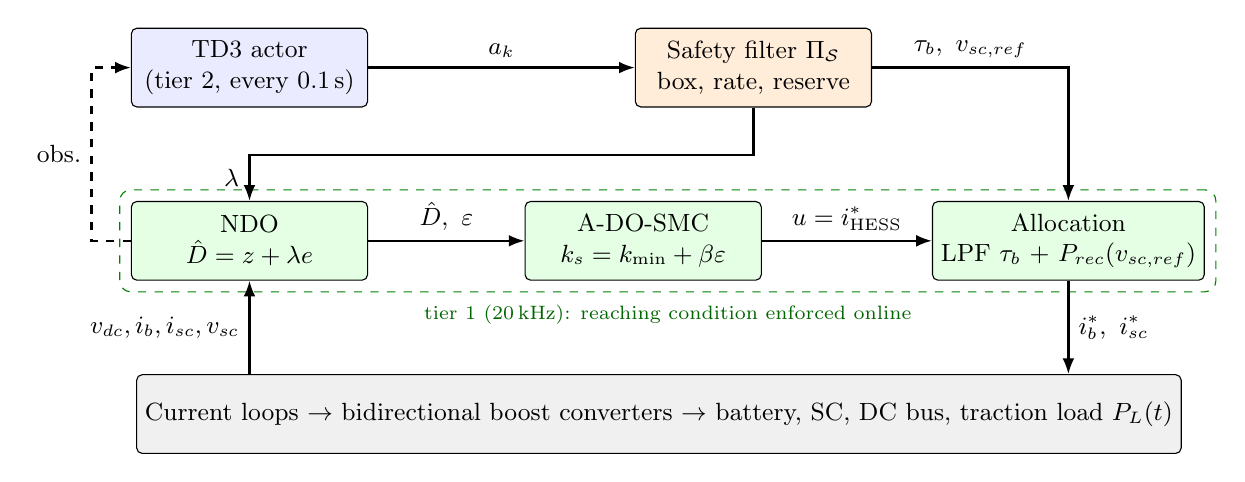
\begin{tikzpicture}[font=\small, >={Latex[length=2mm]},
  blk/.style={draw, rounded corners=2pt, align=center, minimum height=10mm, minimum width=30mm, inner sep=3pt},
  arr/.style={->, thick}]
\node[blk, fill=blue!8]   (agent) at (0,3.0)   {TD3 actor\\(tier 2, every 0.1\,s)};
\node[blk, fill=orange!15](filt)  at (6.4,3.0) {Safety filter $\Pi_\mathcal{S}$\\box, rate, reserve};
\node[blk, fill=green!10] (ndo)   at (0,0.8)   {NDO\\$\hat D=z+\lambda e$};
\node[blk, fill=green!10] (smc)   at (5.0,0.8) {A-DO-SMC\\$k_s=k_{\min}+\beta\varepsilon$};
\node[blk, fill=green!10] (alloc) at (10.4,0.8) {Allocation\\LPF $\tau_b$ + $P_{rec}(v_{sc,ref})$};
\node[blk, fill=gray!12, minimum width=128mm] (plant) at (5.2,-1.4) {Current loops $\rightarrow$ bidirectional boost converters $\rightarrow$ battery, SC, DC bus, traction load $P_L(t)$};
\draw[arr] (agent) -- node[above]{$a_k$} (filt);
\draw[arr] (filt.south) -- ++(0,-0.6) -| node[pos=0.75,left]{$\lambda$} (ndo.north);
\draw[arr] (filt.east) -| node[pos=0.25,above]{$\tau_b,\ v_{sc,ref}$} (alloc.north);
\draw[arr] (ndo) -- node[above]{$\hat D,\ \varepsilon$} (smc);
\draw[arr] (smc) -- node[above]{$u=i^*_{\rm HESS}$} (alloc);
\draw[arr] (alloc.south) -- node[right]{$i_b^*,\ i_{sc}^*$} (alloc.south |- plant.north);
\draw[arr] (ndo.south |- plant.north) -- node[left]{$v_{dc}, i_b, i_{sc}, v_{sc}$} (ndo.south);
\draw[arr, dashed] (ndo.west) -- ++(-0.5,0) |- node[pos=0.25,left]{obs.} (agent.west);
\begin{scope}[on background layer]
\node[draw=green!50!black, dashed, rounded corners, fit=(ndo)(smc)(alloc), inner sep=4pt] (t1) {};
\end{scope}
\node[anchor=north, font=\scriptsize, text=green!40!black] at ([yshift=-1pt]t1.south) {tier 1 (20\,kHz): reaching condition enforced online};
\end{tikzpicture}
\caption{Two-tier architecture. Tier 1 regulates the bus voltage and enforces the reaching condition online for any admissible $\theta$. Tier 2 adapts $\theta=(\tau_b,v_{sc,ref},\lambda)$ through a safety filter.}
\label{fig:arch}
\end{figure*}


\subsection{Battery--supercapacitor HESS}
The HESS consists of a Li-ion battery and a supercapacitor (SC), each connected to a common DC bus through a bidirectional boost converter (Fig.~\ref{fig:arch}). With the averaged converter model, the dynamics are
\begin{align}
L_b \dot i_b &= v_b - r_b i_b - (1-d_b)\,v_{dc},\label{eq:ib}\\
L_{sc} \dot i_{sc} &= v_{sc} - r_{sc} i_{sc} - (1-d_{sc})\,v_{dc},\label{eq:isc}\\
C_{dc}\dot v_{dc} &= (1-d_b)\,i_b + (1-d_{sc})\,i_{sc} - P_L(t)/v_{dc},\label{eq:vdc}\\
C_{sc}\dot v_C &= -i_{sc},\qquad \dot{\mathrm{SOC}}_b = -\eta_b i_b/(3600\,Q_b),\label{eq:soc}
\end{align}
where $v_b=\mathrm{OCV}(\mathrm{SOC}_b)-R_0 i_b$ and $v_{sc}=v_C-R_{esr}i_{sc}$ are the terminal voltages, $d_b,d_{sc}\in[0,d_{\max}]$ are duty ratios, and $P_L$ is the traction power (constant-power load, $P_L<0$ during regenerative braking). The inductor currents are limited, $|i_b|\le I_{b,\max}$ and $|i_{sc}|\le I_{sc,\max}$. Parameters (Table~\ref{tab:params}) follow~\cite{ha2026gtsd}; values not reported there are stated as assumptions.

Note that, with $v_b, v_{sc} < v_{dc}$, the averaged boost form \eqref{eq:ib}--\eqref{eq:isc} is required; the form $L\dot i = u\,v_{src}-v_{dc}-ri$ used in~\cite{ha2026gtsd} would need $u>1$ and cannot represent a duty ratio.

\subsection{Control structure}
A cascaded digital controller with sampling period $T_s=\SI{50}{\micro\second}$ and a one-sample computation delay is used. The outer loop computes the total bus-side HESS current $u=i^*_{\mathrm{HESS}}$, the allocation layer splits it into battery and SC references, and PI current loops with voltage feedforward generate the duty ratios. The complete discrete-time structure used for simulation is given in Section~\ref{sec:impl}. Writing $e=v_{dc}-v^*_{dc}$, the outer-loop design model is
\begin{equation}
\dot e = g\,u + D(t),\qquad g = 1/C_{dc,n},\label{eq:edyn}
\end{equation}
where the aggregated disturbance $D$ collects the unmeasured load current, the inner-loop tracking error and all parameter mismatch. The input $u$ is bounded by the instantaneous capability of the two sources, $u\in[u_{\min},u_{\max}]$, with $u_{\max}=(v_bI_{b,\max}+v_{sc}I_{sc,\max})/v_{dc}$ and $u_{\min}$ defined analogously.

\subsection{Allocation with SC energy recovery}
With $P^*=v_{dc}u$, the battery share is the low-pass component plus an SC energy-recovery term,
\begin{align}
\tau_b\dot P_{b,f} &= P^*-P_{b,f},\label{eq:lpf}\\
P_{rec} &= \mathrm{sat}_{P_{rec,\max}}\!\Big(k_E\,\tfrac{1}{2}C_{sc}\big(v_{sc,ref}^2-v_{sc}^2\big)\Big),\label{eq:prec}
\end{align}
This is followed by saturation of the battery share, assignment of the remainder to the SC within its limits, and re-assignment of any SC shortfall to the battery. Re-assignment is necessary: in the reproduction of~\cite{ha2026gtsd} the literal allocation (SC reference computed from the unsaturated battery reference) caused a bus collapse for every outer-loop controller when the battery limit became active.

\subsection{Problem statement}
The supervisory parameters $\theta=(\tau_b, v_{sc,ref}, \lambda)$, where $\lambda$ is the disturbance-observer gain introduced below, determine how transient power is shared and how much energy the SC holds in reserve. The best $\theta$ depends on the driving situation (Section~\ref{sec:results}). The problem is to adapt $\theta$ online so as to reduce battery stress and power-deficit events, while guaranteeing that the fast voltage loop keeps its stability certificate for \emph{every} admissible $\theta$ trajectory.

\section{Proposed Two-Tier Control Strategy}\label{sec:method}
The proposed controller has two tiers (Fig.~\ref{fig:arch}).
\begin{itemize}
\item \emph{Tier 1} (Section~\ref{sec:tier1}) is a disturbance-observer sliding-mode controller whose switching gain is adapted so that the reaching condition is enforced online.
\item \emph{Tier 2} (Section~\ref{sec:tier2}) is a reinforcement-learning supervisor that adapts the power-sharing and observer parameters through a safety filter.
\end{itemize}
Section~\ref{sec:impl} gives the complete discrete-time structure used for simulation.

\subsection{Tier 1: certificate-enforcing adaptive DO-SMC}\label{sec:tier1}

\subsubsection{Disturbance observer and its error signal}
The nonlinear disturbance observer (NDO) of~\cite{ha2026gtsd},
\begin{equation}
\Dh = z + \lambda e,\qquad \dot z = -\lambda z - \lambda\,(g u + \lambda e),\label{eq:ndo}
\end{equation}
gives $\dot{\Dh} = \lambda(D-\Dh) = \lambda\Dt$ and $\dot{\Dt}=\dot D-\lambda\Dt$ for constant $\lambda$. Hence, under $|\dot D|\le\rho_D$,
\begin{equation}
|\Dt(t)|\le |\Dt(t_0)|e^{-\lambda(t-t_0)}+\rho_D/\lambda.\label{eq:ndobound}
\end{equation}
When the supervisor changes $\lambda$ from $\lambda^-$ to $\lambda^+$, the auxiliary state is re-initialised as $z^+=\Dh^- - \lambda^+e$. This keeps $\Dh$, and therefore $\Dt$, continuous, so \eqref{eq:ndobound} holds piecewise with $\lambda\ge\lambda_{\min}$.

The identity $\dot{\Dh}=\lambda\Dt$ is the key observation used here: \emph{the observer reveals its own estimation error.} We form the estimate
\begin{align}
\hat\varepsilon(t)&=\frac{1}{\lambda}\Big|\mathcal{F}_{\tau_f}\big[\dot{\Dh}\big](t)\Big|,\nonumber\\
\varepsilon(t)&=\max\big(\hat\varepsilon(t),\ \varepsilon(t^-)e^{-T_s/\tau_{env}}\big),\label{eq:env}
\end{align}
where $\mathcal{F}_{\tau_f}$ is a first-order filter (backward difference followed by a \SI{2}{\milli\second} low-pass) and $\varepsilon$ is a decaying peak envelope.

\subsubsection{Sliding surface and control law}
With the integral sliding variable $s=e+c_v\xi$, the control law is
\begin{align}
u &= \mathrm{sat}_{[u_{\min},u_{\max}]}\Big(\tfrac{1}{g}\big(-\Dh - c_v e\nonumber\\
&\qquad - k_s(t)\,\mathrm{sat}(s/\phi_s(t))\big)\Big),\label{eq:law}\\
k_s(t) &= k_{\min}+\beta\,\varepsilon(t),\qquad \phi_s(t)=k_s(t)/k',\label{eq:ks}\\
\dot\xi &= \begin{cases} e, & |s|\le\phi_s \text{ and no input saturation},\\ 0, & \text{otherwise},\end{cases}\label{eq:condint}
\end{align}
with $\beta>1$ and a constant boundary-layer slope $k'$. Two properties follow directly.

\noindent(i) \emph{Fixed small-signal dynamics.} Inside the boundary layer, $k_s\,\mathrm{sat}(s/\phi_s)=k's$ does not depend on $k_s(t)$. The linearised closed loop therefore keeps the poles $\{-c_v,-k'\}$ for any gain trajectory, so the adaptation cannot destabilise the small-signal behaviour.

\noindent(ii) \emph{Online enforcement of the reaching condition.} The sufficient condition $k_s>|\Dt|_{\max}$ of~\cite{ha2026gtsd} (its Eq.~(38)) is replaced by $k_s(t)\ge\beta\varepsilon(t)+k_{\min}$, which tracks the actual estimation error. The conditional integrator~\eqref{eq:condint} removes the windup observed with a fixed small $k_s$.

\begin{assumption}\label{as:est}
There is $\delta\ge 0$ with $|\Dt(t)|\le\beta\varepsilon(t)+\delta$ for all $t\ge t_0$, and $k_{\min}>\delta$.
\end{assumption}

\begin{proposition}\label{prop:uub}
Let Assumption~\ref{as:est} hold, the input be unsaturated, and $\lambda(t)\ge\lambda_{\min}$ be piecewise constant with bumpless switching. Then $s$ reaches the set $|s|\le\bar\phi$ in finite time, where $\bar\phi=\sup_t\max(\phi_s(t),\,\sup|\Dt|/k')$, and remains there. Consequently, $e$ and $\xi$ are uniformly ultimately bounded.
\end{proposition}
\begin{proof}[Proof sketch]
From \eqref{eq:edyn}, \eqref{eq:law}, $\dot s=-k_s\,\mathrm{sat}(s/\phi_s)+\Dt$. With $V=\tfrac12 s^2$ and $|s|>\phi_s$: $\dot V\le-(k_s-|\Dt|)|s|\le-(k_{\min}-\delta)|s|<0$, which gives finite-time reaching of the boundary layer. Inside the layer, $\dot s=-k's+\Dt$ is a stable first-order system driven by the bounded input $\Dt$ from \eqref{eq:ndobound}, so $|s|$ is ultimately bounded by $\sup|\Dt|/k'$. On $|s|\le\bar\phi$ the conditional integrator is active, so $\dot s=\dot e+c_v e$, i.e.\ $\dot e=-c_v e+\dot s$. This is input-to-state stable with respect to $\dot s=-k's+\Dt$, which is bounded. Hence $e$ is uniformly ultimately bounded, and so is $\xi=(s-e)/c_v$. A complete proof that also treats input saturation and the discretisation is left as an open item.
\end{proof}

Assumption~\ref{as:est} is an assumption about the estimator and is \emph{checked numerically}. In the GTSD transient scenario, $k_s(t)\ge|\Dt(t)|$ holds during \AssumptionHoldPct\ of the time (Section~\ref{sec:results}).

\subsection{Tier 2: Safety-Filtered TD3 Supervisor}\label{sec:tier2}

\subsubsection{Markov Decision Process Formulation}
Every $\Delta_a=\SI{0.1}{\second}$ the supervisor observes an 11-dimensional vector built only from signals that the controller already has:
\begin{itemize}
\item the RMS bus-voltage error over the last decision interval;
\item $\Dh$ and its means over the last \SI{1}{\second} and \SI{5}{\second}, which act as a load proxy without a load-current sensor;
\item the SC SOC and the battery current;
\item the current $\theta$;
\item the fraction of time with input saturation;
\item the envelope $\varepsilon$.
\end{itemize}
The actor outputs $a\in[-1,1]^3$, mapped to $\theta$ (logarithmically for $\tau_b$). The reward penalizes battery stress, bus-voltage error, saturation (power deficit), and SC-voltage excursions:
\begin{multline}
r=-\min\!\Big(w_v\tfrac{\overline{e^2}}{e_{\rm ref}^2}+w_b\tfrac{\overline{i_b^2}}{I_{b,\max}^2}+w_s\tfrac{\overline{(\Delta i_b/\Delta t)^2}}{\dot\imath_{\rm ref}^2}\\
+w_{sat}\,\sigma+w_{sc}\,\Pi_{sc},\ r_{\max}\Big),\label{eq:reward}
\end{multline}
where overbars are averages over the decision interval, $\Delta i_b/\Delta t$ is computed from \SI{1}{\milli\second} block means, $\sigma$ is the saturated fraction, and $\Pi_{sc}$ is a quadratic penalty outside $[237.5,368.75]$\,V, a band placed in the SC window as $[190,295]$\,V is in the 150--\SI{300}{V} window of the reduced-storage plant (Section~\ref{sec:res_sizing}). Weights are listed in Table~\ref{tab:params}. The policy is trained with TD3~\cite{fujimoto2018td3}: twin critics, target-policy smoothing, and delayed actor updates, using $2\times64$ ReLU networks. The implementation uses NumPy with manually derived gradients, which were checked against finite differences.

\subsubsection{Safety Filter Design}
Before it is applied, every action passes through the projection
\begin{equation}
\theta_k=\Pi_{\mathcal{S}}\big(\theta_{k-1},\theta(a_k)\big),\label{eq:filter}
\end{equation}
which enforces three sets of constraints.
\begin{enumerate}
\item \emph{Box constraints:} $\tau_b\in[0.05,5]$\,s, $v_{sc,ref}\in[250,362.5]$\,V and $\lambda\in[100,800]$\,s$^{-1}$, so that $\lambda T_s\le0.04$ keeps the discretized observer well inside its stability region.
\item \emph{Rate limits:} $|\Delta\ln\tau_b|\le0.2$, $|\Delta v_{sc,ref}|\le\SI{5}{\volt}$ and $|\Delta\lambda|\le\SI{50}{\per\second}$ per decision. These keep the parameters slowly varying, as required by the piecewise argument of Proposition~\ref{prop:uub}.
\item \emph{Reserve bounds on $v_{sc,ref}$,} described next.
\end{enumerate}

\paragraph{Power-capability reserve bound}
The SC can deliver at most $v_{sc}I_{sc,\max}$, and the battery at most $P_{b,\max}=v_bI_{b,\max}$. Hence the rated traction power $P_{trac,\max}$ can be met only while
\begin{equation}
v_{sc}\ \ge\ v_{pow}=\frac{P_{trac,\max}-P_{b,\max}}{I_{sc,\max}}.\label{eq:vpow}
\end{equation}
Condition \eqref{eq:vpow} is a \emph{power-capability} condition. It is independent of how much energy the SC stores. The proposed filter (v2) requires the SC reference to leave room for the largest contiguous energy deficit $E_{res}$ while still satisfying \eqref{eq:vpow} at the end of that deficit:
\begin{equation}
v_{sc,ref}\ \ge\ \underline v_{sc}=\sqrt{v_{pow}^2+2E_{res}/C_{sc}}.\label{eq:vlo}
\end{equation}
Here $E_{res}=\max\int(P_L-P_{b,\max})^+\,dt$ over contiguous intervals of the \emph{training} cycles. For the Tesla Model 3 plant, $v_{pow}=\MVpow$\,V and $E_{res}=\MEresKJ$\,kJ (on NREL13), which gives $\sqrt{v_{pow}^2+2E_{res}/C_{sc}}\approx\SI{257}{V}$; for the reduced-storage plant the values are \GVpow\,V, \GEresKJ\,kJ and \GVloVtwo\,V. Every quantity in \eqref{eq:vlo} is either a rating or a training-set statistic. As implemented, filter v2 applies the larger of \eqref{eq:vlo} and the v1 bound below.

\paragraph{Filter versions and evaluation protocol}
A first filter (v1) used only an energy reserve of \SI{2}{\second} at the battery-limited deficit,
\[
\underline v_{sc}=\sqrt{v_{sc,\min}^2+2\cdot 2\,(P_{trac,\max}-P_{b,\max})/C_{sc}}.
\] Filter v2 was derived on the reduced-storage plant of the sizing study (Section~\ref{sec:res_sizing}), on which the study was first carried out. There the v1 bound (\GVloVone\,V) lay below the \GBoxLo\,V box limit and was never active, and where the v1 agents lowered the SC reserve and caused power deficits on held-out cycles. Because v2 was motivated by test results, v1 is reported as an ablation and all agents are evaluated on three further cycles that played no role in any design decision. With the Tesla Model 3 plant the v1 bound is \MVloVone\,V, above both the \MBoxLo\,V box limit and the power-capability term of \eqref{eq:vlo}; v1 and v2 are therefore the same filter on this plant, and their agents, trained with the same seeds, are identical.
The tier-1 certificate does not depend on the filter, because \eqref{eq:ks} adapts $k_s$ to whatever $\lambda$ is applied. The filter keeps the \emph{operating assumptions} of the certificate valid, namely slow variation and the bounds on $\lambda$. It also keeps the energy states in a region where the power references remain feasible. This division of responsibility differs from safety filters that act only on the power split~\cite{xu2025safe,wabersich2021psf}. The filter is a projection onto a fixed set (a box with rate limits). Unlike a predictive safety filter~\cite{wabersich2021psf}, it needs no model rollout. Its computational cost is reported in Section~\ref{sec:res_cost}.

\subsubsection{Training and Model-Selection Protocol}
Training uses random \SI{30}{\second} windows of four cycles (UDDS, HWFET, NREL13, a TSDC trip) with randomized initial SC voltage (262.5--356.25\,V), battery SOC (0.5--0.9), and load scale (0.9--1.4). Each agent is trained for 240 episodes (72\,000 transitions). The checkpoint is selected \emph{only} on the validation set (WLTC low; WLTC medium at $\times1.0$ and $\times1.6$). Three training seeds (11, 22, 33) are run for each variant: filter v2 (proposed), filter v1, and no filter. The \emph{no-filter} ablation uses the same reward and network, a wider action box ($\tau_b\in[0.01,20]$\,s, $v_{sc,ref}\in[200,373.75]$\,V, $\lambda\in[20,2000]$\,s$^{-1}$), and no rate or reserve constraints.

\subsection{Digital implementation of the control structure}\label{sec:impl}

This section gives the complete digital control structure in the form used by the simulation. Every equation below corresponds one-to-one to the code in the supplementary archive (\texttt{src/hess/kernel\_sup.py}), and the numerical gains are listed in Table~\ref{tab:ctrl}. The structure is summarized in Fig.~\ref{fig:ctrl}. Three rates are involved:
\begin{itemize}
\item the plant, integrated with fixed-step RK4 at $T_s/5$ or $T_s/10$;
\item the digital controller (tier 1), executed once per switching period $T_s=\SI{50}{\micro s}$;
\item the supervisor (tier 2), executed every $\Delta_a=2000\,T_s=\SI{0.1}{s}$.
\end{itemize}

\begin{figure*}[t]
\centering
\resizebox{\textwidth}{!}{%
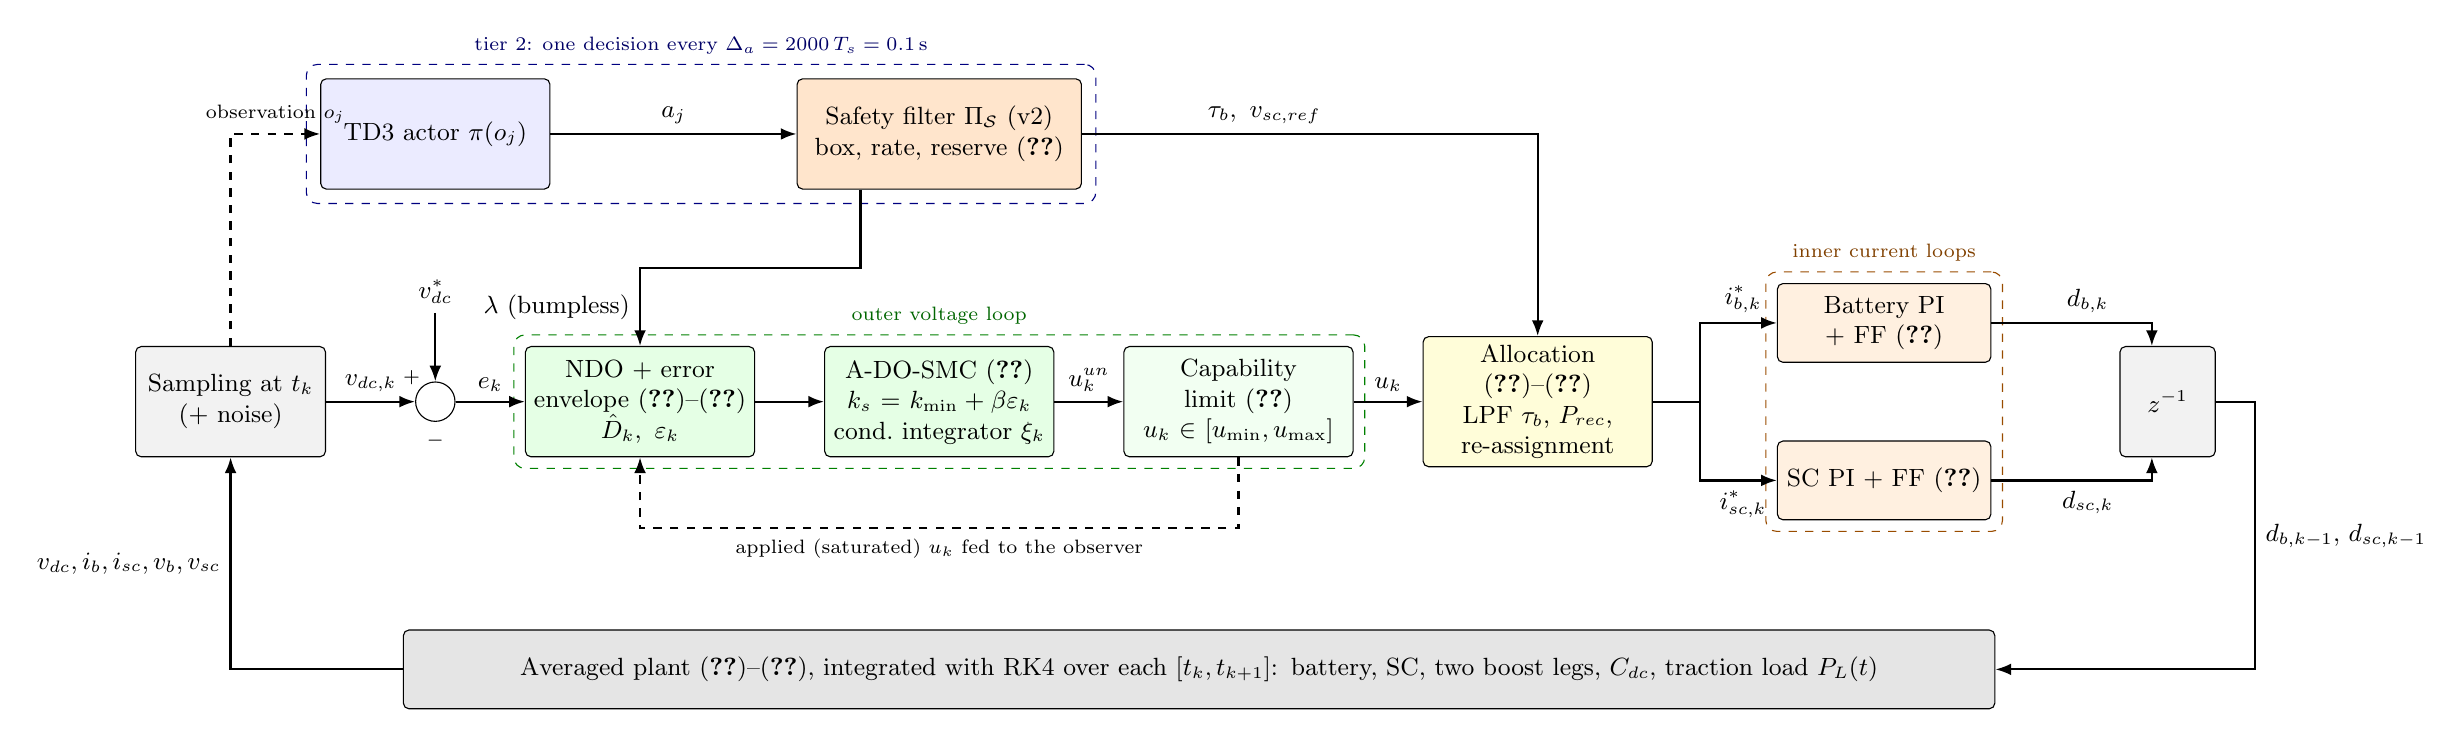
\begin{tikzpicture}[font=\small, >={Latex[length=2mm]},
  blk/.style={draw, rounded corners=2pt, align=center, minimum height=14mm, text width=27mm, inner sep=3pt},
  arr/.style={->, thick}, dsh/.style={->, thick, dashed}]
% ---------------- tier 1 row (one execution per Ts)
\node[blk, fill=gray!10, text width=22mm] (adc) at (0,0) {Sampling at $t_k$\\(+ noise)};
\node[draw, circle, minimum size=5mm, inner sep=0pt] (sum) at (2.6,0) {};
\node at (2.3,0.3) {\scriptsize $+$}; \node at (2.6,-0.5) {\scriptsize $-$};
\node[blk, fill=green!10] (ndo)   at (5.2,0)  {NDO + error envelope \eqref{eq:zdisc}--\eqref{eq:envdisc}\\$\hat D_k,\ \varepsilon_k$};
\node[blk, fill=green!10] (smc)   at (9.0,0)  {A-DO-SMC \eqref{eq:law}\\$k_s=k_{\min}+\beta\varepsilon_k$\\cond.\ integrator $\xi_k$};
\node[blk, fill=green!5]  (lim)   at (12.8,0) {Capability limit \eqref{eq:ulim}\\$u_k\in[u_{\min},u_{\max}]$};
\node[blk, fill=yellow!15](alloc) at (16.6,0) {Allocation \eqref{eq:alloc1}--\eqref{eq:alloc3}\\LPF $\tau_b$, $P_{rec}$, re-assignment};
\node[blk, fill=orange!12, minimum height=10mm, text width=25mm] (pib)  at (21.0,1.0)  {Battery PI + FF \eqref{eq:duty}};
\node[blk, fill=orange!12, minimum height=10mm, text width=25mm] (pisc) at (21.0,-1.0) {SC PI + FF \eqref{eq:duty}};
\node[blk, fill=gray!10, text width=10mm] (dly) at (24.6,0) {$z^{-1}$};
% ---------------- plant row
\node[blk, fill=gray!20, text width=200mm, minimum height=10mm] (plant) at (12.3,-3.4)
  {Averaged plant \eqref{eq:ib}--\eqref{eq:soc}, integrated with RK4 over each $[t_k,t_{k+1}]$: battery, SC, two boost legs, $C_{dc}$, traction load $P_L(t)$};
% ---------------- tier 2 row (every 0.1 s)
\node[blk, fill=blue!8]   (agent) at (2.6,3.4) {TD3 actor $\pi(o_j)$};
\node[blk, fill=orange!20, text width=34mm] (filt) at (9.0,3.4) {Safety filter $\Pi_\mathcal{S}$ (v2)\\box, rate, reserve \eqref{eq:vlo}};
% ---------------- wires tier 1
\node (vref) at (2.6,1.4) {$v^*_{dc}$};
\draw[arr] (vref) -- (sum);
\draw[arr] (adc) -- node[above]{$v_{dc,k}$} (sum);
\draw[arr] (sum) -- node[above]{$e_k$} (ndo);
\draw[arr] (ndo) -- (smc);
\draw[arr] (smc) -- node[above]{$u^{un}_k$} (lim);
\draw[arr] (lim) -- node[above]{$u_k$} (alloc);
\draw[arr] (alloc.east) -- ++(0.6,0) |- node[pos=0.78,above]{$i^*_{b,k}$} (pib.west);
\draw[arr] (alloc.east) -- ++(0.6,0) |- node[pos=0.78,below]{$i^*_{sc,k}$} (pisc.west);
\draw[arr] (pib.east) -| node[pos=0.3,above]{$d_{b,k}$} ([xshift=-2mm]dly.north);
\draw[arr] (pisc.east) -| node[pos=0.3,below]{$d_{sc,k}$} ([xshift=-2mm]dly.south);
\draw[arr] (dly.east) -- ++(0.5,0) |- node[pos=0.25,right]{$d_{b,k-1},\,d_{sc,k-1}$} (plant.east);
\draw[arr] (plant.west) -| node[pos=0.75,left]{$v_{dc},i_b,i_{sc},v_b,v_{sc}$} (adc.south);
\draw[dsh] (lim.south) -- ++(0,-0.9) -| node[pos=0.25,below]{\scriptsize applied (saturated) $u_k$ fed to the observer} (ndo.south);
% ---------------- wires tier 2
\draw[dsh] (adc.north) |- node[pos=0.75,above]{\scriptsize observation $o_j$} (agent.west);
\draw[arr] (agent) -- node[above]{$a_j$} (filt);
\draw[arr] ([xshift=-10mm]filt.south) -- ++(0,-1.0) -| node[pos=0.75,left]{$\lambda$ (bumpless)} (ndo.north);
\draw[arr] (filt.east) -| node[pos=0.2,above]{$\tau_b,\ v_{sc,ref}$} (alloc.north);
% ---------------- groups
\begin{scope}[on background layer]
\node[draw=green!50!black, dashed, rounded corners, fit=(ndo)(smc)(lim), inner sep=4pt,
      label={[green!40!black,font=\scriptsize]above:outer voltage loop}] {};
\node[draw=orange!60!black, dashed, rounded corners, fit=(pib)(pisc), inner sep=4pt,
      label={[orange!50!black,font=\scriptsize]above:inner current loops}] {};
\node[draw=blue!50!black, dashed, rounded corners, fit=(agent)(filt), inner sep=5pt,
      label={[blue!40!black,font=\scriptsize]above:tier 2: one decision every $\Delta_a=2000\,T_s=\SI{0.1}{s}$}] {};
\end{scope}
\end{tikzpicture}}
\caption{Complete control structure as implemented. The middle row (tier 1) is executed once per sampling period $T_s=\SI{50}{\micro s}$ (Algorithm~\ref{alg:tier1}); all measured signals of the sampling block are available to every tier-1 block. The duty ratios computed at $t_k$ are applied one period later ($z^{-1}$). The observer uses the applied (saturated) command $u_k$, and the integral state $\xi_k$ is frozen outside the boundary layer and during saturation. The supervisor (top) acts only through $\lambda$, $\tau_b$ and $v_{sc,ref}$. For the PI and robust-MPC baselines, the A-DO-SMC block is replaced by the corresponding law; all other blocks are unchanged.}
\label{fig:ctrl}
\end{figure*}

\subsubsection{Discrete-time tier-1 equations}
At sample $k$, the controller reads $v_{dc,k}$, $i_{b,k}$, $i_{sc,k}$ and the terminal voltages $v_{b,k}$, $v_{sc,k}$ (true values plus white noise). It then evaluates, in this order:

\paragraph{Capability limits} With the SC limits disabled at the SC voltage bounds ($I^{dis}_{sc}=0$ if $v_{sc,k}\le v_{sc,\min}$, $I^{ch}_{sc}=0$ if $v_{sc,k}\ge v_{sc,\max}$, otherwise $I_{sc,\max}$):
\begin{align}
u_{\max}&=\frac{v_{b,k}I_{b,\max}+v_{sc,k}I^{dis}_{sc}}{v_{dc,k}},\nonumber\\
u_{\min}&=-\frac{v_{b,k}I_{b,\max}+v_{sc,k}I^{ch}_{sc}}{v_{dc,k}}.\label{eq:ulim}
\end{align}

\paragraph{Observer and error envelope} Forward-Euler discretization of \eqref{eq:ndo} and \eqref{eq:env} gives
\begin{align}
\hat D_k&=z_k+\lambda e_k,\nonumber\\
z_{k+1}&=z_k+T_s\big[-\lambda z_k-\lambda(u_k/C_{dc,n}+\lambda e_k)\big],\label{eq:zdisc}\\
\eta_k&=\eta_{k-1}+\tfrac{T_s}{\tau_f}\Big(\tfrac{\hat D_k-\hat D_{k-1}}{T_s}-\eta_{k-1}\Big),\nonumber\\
\varepsilon_k&=\max\!\big(|\eta_k|/\lambda,\ \varepsilon_{k-1}e^{-T_s/\tau_{env}}\big).\label{eq:envdisc}
\end{align}
Because $\lambda T_s\le0.04$ (Section~\ref{sec:tier2}), the Euler observer keeps its pole at $1-\lambda T_s\in[0.96,0.995]$.

\paragraph{Outer law and anti-windup} The unsaturated command $u^{un}_k$ follows from \eqref{eq:law} with $k_s=k_{\min}+\beta\varepsilon_k$ and $\phi_s=k_s/k'$. The applied command is $u_k=\mathrm{sat}_{[u_{\min},u_{\max}]}(u^{un}_k)$. The integral state is updated as $\xi_{k+1}=\xi_k+T_se_k$ only if two conditions hold:
\begin{itemize}
\item $|s_k|\le\phi_s$ (conditional integrator);
\item $u_k=u^{un}_k$ or $(u^{un}_k-u_k)e_k>0$ (integration that drives the command back into range).
\end{itemize}
The same saturation and anti-windup rule is applied to the PI and MPC baselines.

\paragraph{Allocation} With $P^*_k=v_{dc,k}u_k$ and $P_{b,\max}=v_{b,k}I_{b,\max}$:
\begin{align}
P_{b,f,k}&=P_{b,f,k-1}+\tfrac{T_s}{\tau_b}\big(P^*_k-P_{b,f,k-1}\big),\label{eq:alloc1}\\
P_{b1,k}&=\mathrm{sat}_{\pm P_{b,\max}}\big(P_{b,f,k}+P_{rec,k}\big),\nonumber\\
P_{sc,k}&=\mathrm{sat}_{[-v_{sc,k}I^{ch}_{sc},\,v_{sc,k}I^{dis}_{sc}]}\big(P^*_k-P_{b1,k}\big),\label{eq:alloc2}\\
P_{b,k}&=\mathrm{sat}_{\pm P_{b,\max}}\big(P^*_k-P_{sc,k}\big),\nonumber\\
i^*_{b,k}&=P_{b,k}/v_{b,k},\qquad i^*_{sc,k}=P_{sc,k}/v_{sc,k},\label{eq:alloc3}
\end{align}
with $P_{rec,k}$ from \eqref{eq:prec} evaluated at $v_{sc,k}$. The low-pass state is updated before it is used. The expression for $P_{b,k}$ re-assigns to the battery any power the SC cannot supply.

\paragraph{Inner current loops} For each source $x\in\{b,sc\}$, a PI acting on the inductor-voltage demand with source-voltage feedforward gives
\begin{align}
d^{un}_{x,k}&=1-\frac{v_{x,k}-\big(K_{p,x}(i^*_{x,k}-i_{x,k})+I_{x,k}\big)}{v_{dc,k}},\nonumber\\
d_{x,k}&=\mathrm{sat}_{[0,d_{\max}]}(d^{un}_{x,k}).\label{eq:duty}
\end{align}
The integrator is updated as $I_{x,k+1}=I_{x,k}+T_sK_{i,x}(i^*_{x,k}-i_{x,k})$ only when $d_{x,k}=d^{un}_{x,k}$. The duty ratios computed at $t_k$ are held on $[t_{k+1},t_{k+2})$ (one-sample computation delay), and the averaged plant is integrated over each period with these values held constant.

\begin{table*}[t]
\centering\footnotesize\setlength{\tabcolsep}{5pt}
\caption{Controller structure parameters as implemented. D: derived from other parameters by the stated formula; P: from~\cite{ha2026gtsd}; A: assumed.}
\label{tab:ctrl}
\begin{tabular}{@{}p{0.42\textwidth}p{0.45\textwidth}c@{}}
\toprule
Quantity & Value & Src.\\
\midrule
\multicolumn{3}{@{}l}{\emph{Timing}}\\
Controller sampling $T_s$ (= PWM period) & \SI{50}{\micro s} (\SI{20}{kHz}) & A\\
Computation delay & one sample ($d_k$ applied on $[t_{k+1},t_{k+2})$) & A\\
Plant integration (RK4) step & $T_s/5$ (cycles), $T_s/10$ (GTSD profiles) & A\\
Supervisor period $\Delta_a$ & \SI{0.1}{s} $=2000\,T_s$ & A\\
\multicolumn{3}{@{}l}{\emph{Inner current loops}}\\
Bandwidth $\omega_{ci}$ & 5026.5\,rad/s ($2\pi\cdot800$\,Hz) & A\\
$K_{p,b}=L_{b,n}\omega_{ci}$, $K_{i,b}=K_{p,b}\omega_{ci}/5$ & 7.540\,V/A, 7580\,V/(A\,s) & D\\
$K_{p,sc}=L_{sc,n}\omega_{ci}$, $K_{i,sc}=K_{p,sc}\omega_{ci}/5$ & 5.027\,V/A, 5053\,V/(A\,s) & D\\
Duty limits & $0\le d\le 0.95$ & A\\
\multicolumn{3}{@{}l}{\emph{Outer voltage loop (all variants share poles $\{-c_v,-k'\}$)}}\\
A-DO-SMC: $c_v$, $k'$, $k_{\min}$, $\beta$ & 100\,s$^{-1}$, 240\,s$^{-1}$, 120\,V/s, 1.5 & P/A\\
A-DO-SMC: $\tau_f$, $\tau_{env}$ & 2\,ms, 50\,ms & A\\
PI: $K_P=C_{dc,n}(c_v+k')$, $K_I=C_{dc,n}c_vk'$ & 0.748\,A/V, 52.8\,A/(V\,s) & D\\
MPC: $N$, $Q$, $R$ & 20, diag$(6.76\times10^{4}, 5.76\times10^{8})$, 1 & D\\
MPC: LQR gain $K$ on $(e,\xi)$ & [338.3, 23797] & D\\
MPC: tightening at stage $N$ & 571\,V/s ($1.26$\,A) & D\\
\multicolumn{3}{@{}l}{\emph{Allocation}}\\
$k_E$, $P_{rec,\max}$ & 0.02\,s$^{-1}$, 5\,kW & A\\
\bottomrule
\end{tabular}
\end{table*}


\begin{algorithm}[t]
\caption{Tier-1 controller step at sample $k$ (executed every $T_s$)}\label{alg:tier1}
\SetKwInOut{Input}{input}\SetKwInOut{Output}{output}
\Input{$v_{dc,k},i_{b,k},i_{sc,k},v_{b,k},v_{sc,k}$; parameters $\theta=(\tau_b,v_{sc,ref},\lambda)$}
\Output{$d_{b,k},d_{sc,k}$ (applied at $k+1$)}
$e_k\leftarrow v_{dc,k}-v^*_{dc}$; compute $u_{\min},u_{\max}$ by \eqref{eq:ulim}\;
$\hat D_k\leftarrow z_k+\lambda e_k$; update $\eta_k,\varepsilon_k$ by \eqref{eq:envdisc}\;
$k_s\leftarrow k_{\min}+\beta\varepsilon_k$; $\phi_s\leftarrow k_s/k'$; $s_k\leftarrow e_k+c_v\xi_k$\;
$u^{un}_k\leftarrow C_{dc,n}\big(-\hat D_k-c_ve_k-k_s\,\mathrm{sat}(s_k/\phi_s)\big)$; $u_k\leftarrow\mathrm{sat}_{[u_{\min},u_{\max}]}(u^{un}_k)$\;
\lIf{$|s_k|\le\phi_s$ \textbf{and} ($u_k=u^{un}_k$ \textbf{or} $(u^{un}_k-u_k)e_k>0$)}{$\xi_{k+1}\leftarrow\xi_k+T_se_k$}
$z_{k+1}\leftarrow z_k+T_s[-\lambda z_k-\lambda(u_k/C_{dc,n}+\lambda e_k)]$\;
compute $i^*_{b,k},i^*_{sc,k}$ by \eqref{eq:alloc1}--\eqref{eq:alloc3}\;
\ForEach{$x\in\{b,sc\}$}{compute $d_{x,k}$ by \eqref{eq:duty}; \lIf{not clipped}{$I_{x,k+1}\leftarrow I_{x,k}+T_sK_{i,x}(i^*_{x,k}-i_{x,k})$}}
\end{algorithm}

\begin{algorithm}[t]
\caption{Closed-loop simulation with the tier-2 supervisor}\label{alg:sim}
initialize plant state, $v_{dc}=v^*_{dc}$, duties at their steady-state values, controller memories to zero, $\theta_0=(0.2\,\mathrm{s},\SI{250}{V},\SI{250}{s^{-1}})$\;
\For{$j=0,1,\dots$ (decision instants $t=j\Delta_a$)}{
build observation $o_j$ (Section~\ref{sec:tier2}); $a_j\leftarrow\pi(o_j)$\;
$\theta_j\leftarrow\Pi_\mathcal{S}(\theta_{j-1},\theta(a_j))$ \tcp*{box, rate, reserve}
\If{$\lambda$ changes}{$z\leftarrow\hat D-\lambda_{new}e$ \tcp*{bumpless: keeps $\hat D$ continuous}}
\For{$k=2000j,\dots,2000j+1999$}{
sample measurements with noise; run Algorithm~\ref{alg:tier1}\;
apply $d_{\cdot,k-1}$ and integrate the plant over $[t_k,t_{k+1}]$ with RK4 (5 or 10 substeps)\;
accumulate the indices of Section~\ref{sec:setup} from the true signals\;
\lIf{$v_{dc}\notin[0.5,1.5]\,v^*_{dc}$}{stop and mark the run as failed}
}
compute reward \eqref{eq:reward} (training only)\;
}
\end{algorithm}

\paragraph{Verification of the implementation} The implementation was checked in four ways, with the results stored in the archive:
\begin{itemize}
\item \emph{Energy balance.} The change in stored energy matched the source energy minus the losses and the load energy, with a relative residual of $\EnergyResidual$.
\item \emph{Switching model.} A switched-PWM version of the plant reproduced the analytic inductor ripple $v\,d\,T_s/L$ within 3\,\%.
\item \emph{Step size.} Reducing the RK4 step by a factor of four changed the reported indices by a relative amount below \TimestepRelPct.
\item \emph{Chunked execution.} Running the simulation in supervisor-length chunks reproduced the uninterrupted run within 1\,\% for every outer loop.
\end{itemize}


\section{Simulation Results and Discussion}\label{sec:results}
This section first describes the simulation setup (Section~\ref{sec:setup}). It then reports, in order:
\begin{itemize}
\item the reproduction of the fixed-gain DO-SMC that motivates this work (Section~\ref{sec:repro});
\item the tier-1 results (Section~\ref{sec:res_tier1});
\item the training, held-out test, safety-filter ablation, additional-cycle and computational-cost results of tier 2 (Sections~\ref{sec:res_train}--\ref{sec:res_cost}).
\end{itemize}
It closes with a discussion of mechanisms, trade-offs and limits (Section~\ref{sec:discussion}).

\subsection{Simulation Setup}\label{sec:setup}



\begin{table*}[t]
\centering\footnotesize\setlength{\tabcolsep}{4pt}
\caption{Plant and controller parameters. All results use the Tesla Model 3 plant except the storage-sizing sensitivity study (Section~\ref{sec:res_sizing}), which uses the reduced-storage plant. Sources: M3 measured on a Tesla Model 3 SR+ (2020, LFP)~\cite{rosenberger2024m3}; F FASTSim Model 3 file~\cite{fastsimrepo}; MX ultracapacitor datasheet~\cite{maxwell125v}; D sized in this work by the stated rule (the production Model 3 has no SC and no battery DC--DC stage); A assumed.}
\label{tab:params}
\begin{tabular}{@{}p{0.20\textwidth}p{0.24\textwidth}p{0.41\textwidth}l@{}}
\toprule
Quantity & Reduced-storage plant (A) & Tesla Model 3 plant & Src.\\\midrule
Vehicle mass, rotational factor & \SI{1600}{kg}, 1.05 & \SI{1830}{kg} (\SI{1755}{kg} measured + \SI{75}{kg} driver), 1.06 & M3\\
Road load & $C_dA=\SI{0.644}{m^2}$, $C_{rr}=0.009$ & coast-down $F=177.2+5.743v+0.2538v^2$\,N ($v$ in m/s) & M3\\
Peak traction / regenerative power & \SI{60}{kW} / \SI{30}{kW} & \SI{239}{kW} / \SI{66.9}{kW} & M3\\
Drive-unit efficiency, auxiliary load & 0.9 / $0.7\times0.8$, \SI{1}{kW} & 0.9 motoring and generating, all braking regenerative; \SI{0.25}{kW} & A; F\\
Battery & \SI{300}{V}, \SI{40}{Ah}, $R_0=\SI{80}{m\ohm}$ & LFP 106s1p, \SI{161}{Ah}, OCV 327.4--\SI{364.3}{V} (linear), $R_0=106\times\SI{0.79}{m\ohm}=\SI{83.7}{m\ohm}$ & M3\\
Supercapacitor & \SI{120}{F}, 150--\SI{300}{V}, $R_{esr}=\SI{10}{m\ohm}$ & 3 modules in series: \SI{21}{F}, 187.5--\SI{375}{V}, $R_{esr}=\SI{54}{m\ohm}$ & MX; D\\
Current limits $I_{b,\max}$, $I_{sc,\max}$ & \SI{80}{A}, \SI{180}{A} & \SI{161}{A} (1C), \SI{800}{A} (module abs.\ max.\ \SI{1900}{A}) & D\\
$v^*_{dc}$, $C_{dc}$, $L_b$, $L_{sc}$ & \SI{400}{V}, \SI{2.2}{mF}, \SI{1.5}{mH}, \SI{1.0}{mH} & \SI{500}{V}, \SI{4.7}{mF}, \SI{0.2}{mH}, \SI{0.05}{mH} (ripple $\le20\,\%$ of the limit at \SI{20}{kHz}) & D\\
Converter resistances $r_b$, $r_{sc}$ & \SI{30}{m\ohm}, \SI{20}{m\ohm} & \SI{10}{m\ohm}, \SI{5}{m\ohm} & A\\
Fixed supervisor $\tau_b$, $v_{sc,ref}$; $k_E$, $P_{rec,\max}$ & \SI{0.2}{s}, \SI{250}{V}; \SI{0.02}{s^{-1}}, \SI{5}{kW} & \SI{0.2}{s}, \SI{312.5}{V}; \SI{0.02}{s^{-1}}, \SI{12}{kW} (same relative values) & A\\
\midrule
\multicolumn{4}{@{}l}{\emph{Common to both plants}}\\
$\lambda$ (nominal), $k_{\min}$, $k'$ & \multicolumn{2}{l}{\SI{250}{s^{-1}}, \SI{120}{V/s}, \SI{240}{s^{-1}} (A)} & \\
$c_v$, $\beta$, $\tau_f$, $\tau_{env}$ & \multicolumn{2}{l}{\SI{100}{s^{-1}}, 1.5, \SI{2}{ms}, \SI{50}{ms} (A)} & \\
$T_s$, plant step; noise $\sigma_v$, $\sigma_i$ & \multicolumn{2}{l}{\SI{50}{\micro s}, $T_s/5$, RK4; \SI{0.2}{V}, \SI{0.2}{A} (A)} & \\
Reward $w_v,w_b,w_s,w_{sat},w_{sc}$; $e_{\rm ref}$, $\dot\imath_{\rm ref}$, $r_{\max}$ & \multicolumn{2}{l}{0.5, 1, 0.5, 5, 2; \SI{5}{V}, \SI{500}{A/s}, 10 (A)} & \\
TD3: $\gamma$, $\tau$, lr, batch & \multicolumn{2}{l}{0.98, 0.005, $3{\times}10^{-4}$, 128 (A)} & \\\bottomrule
\end{tabular}
\end{table*}

\paragraph{Plant and solver}
Equations \eqref{eq:ib}--\eqref{eq:soc} are integrated with fixed-step RK4. The step is \SI{10}{\micro\second}; reducing the step to \SI{2.5}{\micro\second} changed the reported indices by a relative amount below \TimestepRelPct. Measurements carry white noise. The controller is digital with a one-sample delay.

\paragraph{Load profiles}
Speed traces of standard cycles are taken from the FASTSim repository at a pinned commit~\cite{brooker2015fastsim,fastsimrepo}. They are interpolated with a shape-preserving spline and converted to bus power with the measured coast-down road load, mass and rotational-inertia factor of a Tesla Model 3~\cite{rosenberger2024m3} (Table~\ref{tab:params}), a constant drive-unit efficiency, and clipping to the measured peak traction and regenerative powers. The production Model 3 connects its LFP pack directly to the inverter. Here the same pack feeds the bus through a bidirectional converter limited to 1C (\SI{161}{A}), and a three-module ultracapacitor bank~\cite{maxwell125v} supplies the remainder; this HESS is a design study on the Model 3 vehicle and battery, not a description of the production car. The mass of the SC bank is not added to the vehicle mass; its effect is evaluated in Section~\ref{sec:res_loss}. The test set contains five items that were never used for training or checkpoint selection: US06 ($\times1.0$, $\times1.1$), WLTC high, and WLTC extra-high ($\times1.0$, $\times1.2$). Three further cycles (WMTC, FTP-MC1b, and the first \SI{1200}{s} of a long-haul trace) were added only after filter v2 had been fixed; no design decision depends on them.

\paragraph{Compared configurations}
All configurations use the same plant, allocation structure, current loops, limits, and noise realizations (seeds 101--103).
\begin{itemize}
\item \emph{Outer loops:} PI tuned to the same small-signal poles $\{-c_v,-k'\}$; a conventional DO-SMC with the same observer and a fixed switching gain, in two tunings: a low gain $k_s=k_{\min}=\SI{120}{V/s}$ ($\phi_s=\SI{0.5}{V}$), and a high gain $k_s=\KsHi$\,V/s ($\phi_s=k_s/k'=\PhiHi$\,V) sized for the worst case of the training cycles, i.e.\ $1.1$ times the largest observer error logged with A-DO-SMC on the four training cycles, rounded up; an offset-free robust MPC (horizon 20, constraint tightening after~\cite{chisci2001}, LQR terminal cost with the same poles); and the proposed A-DO-SMC.
\item \emph{Supervisors (with A-DO-SMC):} fixed $\theta$; an SOC-adaptive split with $\tau_b$ interpolated between 0.2 and \SI{5}{s} according to the SC SOC, in the spirit of~\cite{nguyen2021adaptive}; a model-predictive energy-management supervisor (MPC-EMS, described below) with two load forecasts; TD3 without a filter; TD3 with filter v1; and TD3 with filter v2 (proposed).
\end{itemize}

\paragraph{Model-predictive energy-management baseline}
To test whether learning is needed at all, we add a non-learning, optimization-based supervisor in the spirit of predictive HESS energy management~\cite{ha2026hmpc,ha2026agsp}. It acts on the same variables as the agent, at the same period $\Delta_a=\SI{0.1}{s}$, and every candidate decision is passed through the same safety filter v2. The observer gain is held at its nominal value, because the energy model below does not depend on it. The prediction model has the structure of the allocation layer \eqref{eq:lpf}--\eqref{eq:prec} and assumes that tier~1 tracks $P^*=P_L$:
\begin{align}
P_{b,f,j+1}&=P_{b,f,j}+\big(1-e^{-\Delta_a/\tau_b}\big)\big(\hat P_{L,j}-P_{b,f,j}\big),\nonumber\\
P_{b,j}&=\mathcal{A}\big(\hat P_{L,j},P_{b,f,j+1},P_{rec}(v_{sc,ref},v_{sc,j})\big),\nonumber\\
v_{sc,j+1}^2&=v_{sc,j}^2-2P_{sc,j}\Delta_a/C_{sc},\label{eq:mpcems}
\end{align}
where $\mathcal{A}$ denotes the saturation and re-assignment steps of Section~\ref{sec:impl} and $P_{sc,j}$ the resulting SC power. The stage cost contains the terms of the reward \eqref{eq:reward} that the model can predict, with the same weights: battery current and its rate of change, a power-deficit indicator (in place of the saturated fraction), and the SC-window penalty $\Pi_{sc}$. The decision is made by enumerating $5\times5=\NCandMPC$ candidate moves $(\Delta\log\tau_b,\Delta v_{sc,ref})$ that span the filter's rate window, each held constant over the horizon (move blocking), and applying the one with the lowest predicted cost. Two load forecasts are compared:
\begin{itemize}
\item \emph{persistence}: $\hat P_{L,j}$ equals the mean of $P^*=v_{dc}u$ over the last decision interval, a causal, controller-internal signal;
\item \emph{preview}: the true future load of the drive cycle. This forecast is non-causal and serves only as an optimistic reference.
\end{itemize}
The horizon was chosen on the validation set from $\{2,5,10\}$\,s with the same protocol as TD3 checkpoint selection. The validation return per decision was \ValMPCPTwo, \ValMPCPFive\ and \ValMPCPTen\ (persistence) and \ValMPCVTwo, \ValMPCVFive\ and \ValMPCVTen\ (preview). A horizon of \HorMPCP\,s was therefore used for both forecasts. No terminal cost on the SC energy is used, so that the MPC-EMS optimizes the same objective that the agent is trained on.

\paragraph{Performance indices}
\begin{itemize}
\item Bus voltage: maximum and RMS deviation.
\item Battery current: RMS value and RMS rate of change computed on \SI{1}{ms} block means.
\item Battery charge throughput (Ah).
\item Saturated fraction: share of samples in which the commanded total current was clipped, i.e., a power deficit.
\item Minimum SC voltage.
\end{itemize}
Every index is computed from the true (noise-free) plant signals.

All results are from offline simulation. Each value is computed by the scripts in the supplementary archive from stored raw logs; no value was entered by hand.

\subsection{Tier-1 Performance of the A-DO-SMC}\label{sec:res_tier1}
\begin{table*}[t]
\centering\footnotesize\setlength{\tabcolsep}{5pt}
\caption{Tier-1 comparison on held-out drive cycles of the Tesla Model 3 plant (fixed supervisor, mean over noise seeds 101--103). The last column is the median time of one controller update on the simulation host.}
\label{tab:tier1}
\begin{tabular}{@{}lccccccc@{}}
\toprule
 & \multicolumn{2}{c}{US06} & \multicolumn{2}{c}{US06$\times1.1$} & \multicolumn{2}{c}{WLTC x-high$\times1.2$} & Update\\
Outer loop & max$|e|$ (V) & RMS $e$ (V) & max$|e|$ (V) & RMS $e$ (V) & max$|e|$ (V) & RMS $e$ (V) & (\si{\micro s})\\
\midrule
PI (same small-signal poles) & 8.47 & 0.628 & 9.30 & 0.690 & 0.63 & 0.090 & \TimePI\\
DO-SMC, low gain ($k_s=120$\,V/s) & 6.95 & 0.367 & 7.75 & 0.421 & 0.18 & 0.033 & \TimeDOSMC\\
DO-SMC, high gain ($k_s=\KsHi$\,V/s) & 1.48 & 0.043 & 1.63 & 0.045 & 0.18 & 0.033 & \TimeDOSMC\\
Robust MPC (offset-free, $N=20$) & 1.48 & 0.044 & 1.63 & 0.045 & 0.18 & 0.034 & \TimeMPC\\
A-DO-SMC (proposed tier 1) & 1.48 & 0.043 & 1.63 & 0.045 & 0.18 & 0.033 & \TimeADOSMC\\
\bottomrule
\end{tabular}
\end{table*}


Table~\ref{tab:tier1} compares five outer loops on the Tesla Model 3 plant with the fixed supervisor, on the three test items with the largest bus deviations.

\paragraph{Fixed low gain}
With $k_s=\SI{120}{V/s}$, the observer error on US06 reaches $|\Dt|_{\max}=\DtLoUSnn$\,V/s in the noise-free run, about \DtLoRatio\ times the switching gain. The reaching condition $k_s>|\Dt|$ holds in steady state (\CondLoFrac\,\% of the samples) but is violated during the strong acceleration and braking transients. Outside the boundary layer the switching term then contributes at most $C_{dc}k_s\approx\SI{0.56}{A}$, and the loop reduces to observer compensation plus the $c_ve$ term. The maximum bus deviation on US06 is \TOneLoUSMax\,V, closer to a PI controller with the same small-signal poles (\TOnePIUSMax\,V) than to the robust MPC (\TOneMPCUSMax\,V).

\paragraph{Adaptive gain}
A-DO-SMC lowers the maximum deviation on US06 to \TOneAUSMax\,V and the RMS deviation from \TOneLoUSRms\ to \TOneAUSRms\,V, the same as the robust MPC, whose QP constraints were never active in these runs, so the MPC acts as an observer-compensated LQR. On US06$\times1.1$ the values are \TOneAUSbMax\,V against \TOneLoUSbMax\,V. On the WLTC cycles all observer-based loops reach about \SI{0.2}{V}, and only PI is worse.

\paragraph{Fixed high gain}
A fixed gain sized for the worst case of the training cycles ($k_s=\KsHi$\,V/s, $\phi_s=\PhiHi$\,V) satisfies the reaching condition on US06 (\CondHiFrac\,\% of the samples, minimum ratio $k_s/|\Dt|=\CondHiMin$) and gives the same regulation as A-DO-SMC on every test item (Table~\ref{tab:tier1}). On the nominal plant, the benefit of A-DO-SMC is therefore not better regulation than a well-sized constant gain. It lies in three properties: the gain does not have to be sized in advance from a worst-case error bound; the condition is enforced for whatever observer gain $\lambda$ a supervisor applies, whereas a fixed gain sized at the nominal $\lambda$ loses its margin when $\lambda$ is lowered, because the bound \eqref{eq:ndobound} on $|\Dt|$ grows as $\rho_D/\lambda$; and the large gain and wide boundary layer are applied only while the observer error is large. At the nominal observer gain the high-gain margin on US06 is small (\CondHiMin); its consequence is tested next.

\paragraph{Robustness to the observer gain}
\begin{table*}[t]
\centering\footnotesize\setlength{\tabcolsep}{4pt}
\caption{Robustness of tier 1 to the observer gain on US06 (Tesla Model 3 plant). Hi: fixed high-gain DO-SMC ($k_s=\KsHi$\,V/s, sized at the nominal $\lambda=\SI{250}{s^{-1}}$); A: A-DO-SMC. Agent rows replay open-loop the schedule $(\tau_b,v_{sc,ref},\lambda)(t)$ chosen by each filter-v2 agent in its evaluation run, so both controllers see the same $\lambda(t)$. max$|e|$: mean over noise seeds 101--103; $r_{\min}=\min_t k_s/|\Dt|$ ($t>0.2$\,s, seed 101, \SI{1}{ms} logging). $^\ddagger$Power deficit (input saturated \LamSatPct\,\% of the time, capability condition (H3) violated).}
\label{tab:lambda}
\begin{tabular}{@{}llcccccccc@{}}
\toprule
 & & \multicolumn{4}{c}{US06} & \multicolumn{4}{c}{US06$\times1.1$}\\\cmidrule(lr){3-6}\cmidrule(lr){7-10}
$\lambda$ schedule & $\lambda$ range (s$^{-1}$) & \multicolumn{2}{c}{max$|e|$ (V)} & \multicolumn{2}{c}{$r_{\min}$} & \multicolumn{2}{c}{max$|e|$ (V)} & \multicolumn{2}{c}{$r_{\min}$}\\
 & & Hi & A & Hi & A & Hi & A & Hi & A\\
\midrule
constant, $\lambda=\lambda_{\min}$ & 100 & 11.40 & 2.71 & 0.554 & 1.316 & 12.04 & 2.98 & 0.508 & 1.320\\
constant, nominal & 250 & 1.48 & 1.48 & 1.101 & 1.252 & 1.63 & 1.63 & 1.026 & 1.250\\
constant, $\lambda=\lambda_{\max}$ & 800 & 0.59 & 0.59 & 2.144 & 1.032 & 0.64 & 0.64 & 2.070 & 1.025\\
\midrule
TD3 agent, seed 11 & 114--746 & 1.58 & 1.58 & 1.167 & 1.090 & 1.96 & 1.96 & 0.997 & 1.093\\
TD3 agent, seed 22 & 121--800 & 0.90 & 0.90 & 1.926 & 1.147 & 0.97 & 0.97 & 1.818 & 1.004\\
TD3 agent, seed 33 & 133--800 & 1.03 & 1.03 & 1.733 & 1.028 & 167.98$^\ddagger$ & 167.85$^\ddagger$ & 0.040 & 0.047\\
\bottomrule
\end{tabular}
\end{table*}

Table~\ref{tab:lambda} tests this property on US06, with the observer gain held at the bounds of the safety filter and at its nominal value, and with the $\lambda$ schedules chosen by the three filter-v2 agents.
\begin{itemize}
\item \emph{Lower bound} ($\lambda=\SI{100}{s^{-1}}$). The observer error grows, and the fixed high gain no longer satisfies the reaching condition ($r_{\min}=\LamHiUSRatio$). The condition fails in only \LamHiUSFail\,\% of the samples, yet the maximum bus deviation rises to \LamHiUSMax\,V (\LamHiUSbMax\,V on US06$\times1.1$). A-DO-SMC raises its gain with the error ($r_{\min}=\LamAUSRatio$) and limits the deviation to \LamAUSMax\,V, \LamFactorHi\ times less.
\item \emph{Nominal value and upper bound.} Both controllers give identical regulation. Whenever the reaching condition holds, both operate inside the boundary layer with the same slope $k'$, so their closed loops coincide.
\item \emph{Agent schedules.} Replaying the agents' schedules open-loop gives identical regulation for both controllers (largest difference \LamAgentMaxDiff\,V outside the deficit run). The agents lowered $\lambda$ to \LamAgentMin\,s$^{-1}$ only briefly and kept it at \LamAgentMeanLo--\LamAgentMeanHi\,s$^{-1}$ on average, above the nominal value. The fixed high gain therefore violated the condition only marginally ($r_{\min}=\LamHiAgentRatioMin$, seed 11 on US06$\times1.1$) and without visible effect. The power deficit of the seed-33 schedule on US06$\times1.1$ violates the capability condition (H3) and affects both controllers equally.
\end{itemize}
The robustness of A-DO-SMC to the observer gain is thus decisive when $\lambda$ is low during strong transients, as at the lower filter bound; the evaluated agents did not operate there, so in the agent runs it was not exercised. With noise, A-DO-SMC kept $k_s\ge|\Dt|$ in all runs without a deficit ($r_{\min}\ge\LamARatioMin$). Several of these ratios are below the value $12/11$ used in Section~\ref{sec:tier1}, so the numerical check of Assumption~\ref{as:est} is not met in every noisy run.

\paragraph{Gain-adaptation mechanism}
Fig.~\ref{fig:tier1} shows the largest transient of US06. In the noise-free run, the envelope raises $k_s(t)$ to $\KsMaxAdapt$\,V/s, above the true observer error ($|\Dt|_{\max}=\DtildeMaxAdapt$\,V/s). The condition $k_s\ge|\Dt|$ holds during \AssumptionHoldPct\ of the run, with a minimum ratio $k_s/|\Dt|$ of \MinKsRatio; since this ratio exceeds $12/11$, Assumption~\ref{as:est} is satisfied in this run (Section~\ref{sec:tier1}). With measurement noise the condition also holds in all logged samples (\SI{1}{ms} resolution, minimum ratio \AsmNoisyMinRatio). In steady state the gain decays toward $k_{\min}$, and the boundary layer $\phi_s=k_s/k'$ shrinks with it. The control law is therefore never high-gain inside the layer: its slope stays at $k'=\SI{240}{s^{-1}}$ throughout.

\paragraph{Computational cost}
One A-DO-SMC update costs \TimeADOSMC\,\si{\micro s}, essentially the same as a fixed-gain DO-SMC (\TimeDOSMC\,\si{\micro s}). The robust MPC costs \TimeMPC\,\si{\micro s} when its constraints are inactive and \TimeMPCActive\,\si{\micro s} when they are active.

\begin{figure*}[t]
\centering
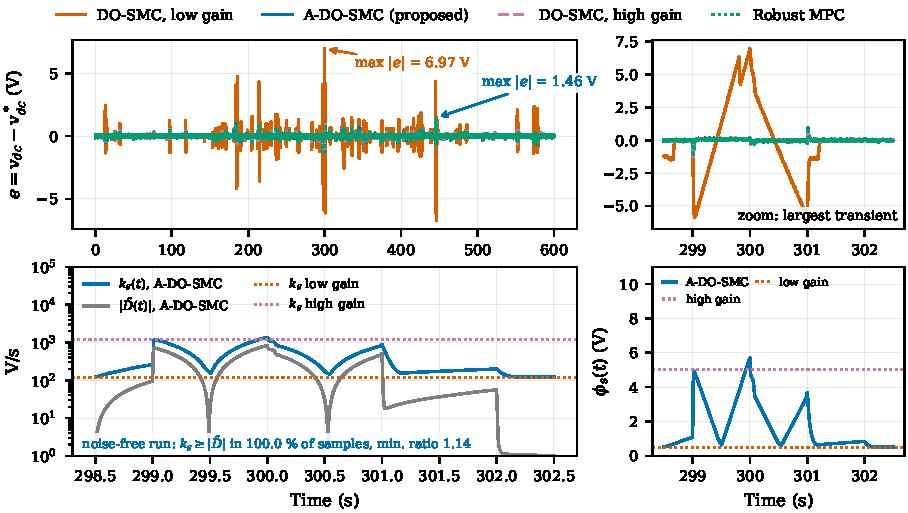
\includegraphics[width=\textwidth]{../results/figures/F2_tier1_m3_us06.pdf}
\caption{US06 on the Tesla Model 3 plant, fixed supervisor, noise seed 101. Top: bus-voltage error for the fixed-gain DO-SMC with low and high gain, the robust MPC and A-DO-SMC over the whole cycle (left) and around the largest transient (right, \ZoomA--\ZoomB\,s). The high-gain DO-SMC and robust MPC curves lie on that of A-DO-SMC. Bottom (noise-free run of A-DO-SMC, same window): adaptive switching gain $k_s(t)$ and true observer error $|\Dt(t)|$, computed from the plant (left, log scale), and boundary-layer width $\phi_s(t)=k_s(t)/k'$ (right); dotted lines: the constant values of the two fixed-gain tunings.}
\label{fig:tier1}
\end{figure*}

\subsection{Tier 2: training and validation}\label{sec:res_train}
\begin{figure}[t]
\centering
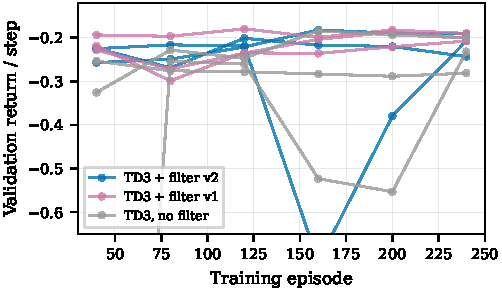
\includegraphics[width=\columnwidth]{../results/figures/F3_validation_curves.pdf}
\caption{Validation return per decision during training (three seeds per variant; evaluated every 40 episodes on WLTC low, WLTC medium, and WLTC medium$\times1.6$). For reference, the fixed and SOC-rule supervisors score \ValFixed\ and \ValRule. Two evaluations fall below the plotted range (no-filter seed 33 at episode 40; filter-v2 seed 33 at episode 160).}
\label{fig:val}
\end{figure}

Fig.~\ref{fig:val} shows the validation return during training. With checkpoint selection on validation only, the selected agents score:
\begin{itemize}
\item filter v2: \ValVtwoSA, \ValVtwoSB, \ValVtwoSC\ (seeds 11, 22, 33);
\item filter v1: \ValVoneSA, \ValVoneSB, \ValVoneSC;
\item no filter: \ValNofSA, \ValNofSB, \ValNofSC.
\end{itemize}
For comparison, the SOC rule scores \ValRule\ and the fixed supervisor \ValFixed. The curves are not monotonic, and one seed of each of the no-filter and v2 variants has a transient collapse. Validation alone would therefore suggest that every filtered agent beats the fixed and rule-based supervisors. The same validation protocol, however, ranks the non-learning MPC-EMS above every agent: \ValMPCPTwo\ with the causal persistence forecast and \ValMPCVTwo\ with preview (Section~\ref{sec:setup}). The test results below show that neither ranking transfers to all unseen cycles.

\subsection{Tier 2: held-out test cycles}\label{sec:res_test}
\input{tab_test.tex}

Table~\ref{tab:test} and Fig.~\ref{fig:testbars} summarize the five test items. All rows share tier 1 (A-DO-SMC). Bus-voltage regulation therefore differs only where the supervisor causes a power deficit.

\begin{figure*}[t]
\centering
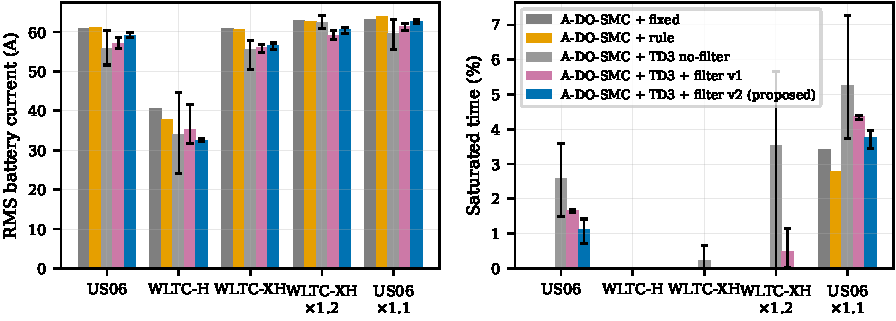
\includegraphics[width=0.9\textwidth]{../results/figures/F5_test_battery_rms_saturation.pdf}
\caption{Held-out test cycles: RMS battery current (left) and fraction of time with the total-current command saturated, i.e., a power deficit (right). Learned supervisors: bar = mean over three training seeds, whisker = min--max.}
\label{fig:testbars}
\end{figure*}

\paragraph{Cycles inside the training power envelope}
On WLTC high and WLTC extra-high, the proposed supervisor (TD3 + filter v2) lowers the RMS battery current in all nine seed pairs, with no saturation:
\begin{itemize}
\item WLTC high: from \R{wh:afix:ibrms}\,A (fixed) and \R{wh:arule:ibrms}\,A (SOC rule) to \R{wh:v2:ibrms:mean}\,A, i.e., \R{wh:v2vsafix:dibrmsabs}\,\% lower than fixed and \R{wh:v2vsarule:dibrmsabs}\,\% lower than the rule;
\item WLTC extra-high: \R{wxa:v2vsafix:dibrmsabs}\,\% lower than fixed.
\end{itemize}
The bus voltage is unaffected: \R{wh:v2:maxdev:mean}\,V versus \R{wh:afix:maxdev}\,V on WLTC high. The price is a higher RMS rate of change of the battery current: \R{wxa:v2vsafix:dslew}\,\% versus fixed on WLTC extra-high.

\paragraph{How the agent achieves this}
The raw logs show that the agents do not use $v_{sc,ref}$ as a slowly varying reserve setpoint, which is how it was intended to be used. Instead, they move it quickly: its standard deviation within a run is \VrefStdMin--\VrefStdMax\,V. As a result, the recovery term \eqref{eq:prec} is at its $\pm\PrecMax$\,kW limit in \CapFracMin--\CapFracMax\,\% of the samples. With the fixed supervisor, the mean $|P_{rec}|$ is only \PrecWHfixedAbs\,kW on WLTC high. In effect, the agent turns the bounded recovery term into a bang-bang actuator for battery power. On transient cycles it switches this power against the load and so lowers the RMS battery current. The agent also keeps $\tau_b$ near its lower bound for most of the run (Fig.~\ref{fig:us06}), which explains the faster battery-current changes.

\paragraph{US06: out of the training envelope}
On US06, the same behavior is harmful. The SC is depleted by long acceleration phases and needs sustained recharging. Here, the switching policy delivers a mean recovery power of only \PrecUSvtwoMin--\PrecUSvtwoMax\,kW (seeds 11, 22, 33), compared with \PrecUSfixed\,kW for the fixed supervisor, which simply recharges at its limit. The SC voltage therefore falls to \R{us06a:v2:vmin:mean}\,V (fixed: \R{us06a:afix:vmin}\,V), below the power-capability level \eqref{eq:vpow}. The command is saturated \R{us06a:v2:sat:mean}\,\% of the time, whereas the fixed supervisor never saturates, and the bus-voltage excursion reaches \R{us06a:v2:maxdev:mean}\,V. This is not a loss of tier-1 stability, since the loop recovers once the demand falls, but it is an operating failure. The \R{us06a:v2vsafix:dibrmsabs}\,\% lower RMS battery current does not compensate for it.

The reserve bound \eqref{eq:vlo} constrains the \emph{reference} $v_{sc,ref}$, not the SC voltage itself, and it is sized using the largest deficit of the training cycles ($E_{res}=\EresKJ$\,kJ). Neither property protects against a policy that keeps the reference high on average while withholding recharge power.

\paragraph{Loads beyond the rating}
With the load scaled by 1.1 (US06) or 1.2 (WLTC extra-high), the peak demand exceeds the vehicle rating used in \eqref{eq:vpow}. On US06$\times1.1$, every configuration saturates: fixed \R{us06b:afix:sat}\,\%, SOC rule \R{us06b:arule:sat}\,\%, v2 \R{us06b:v2:sat:mean}\,\%. On WLTC extra-high$\times1.2$, v2 avoids saturation, as do the fixed and rule supervisors. It still lowers the RMS battery current by \R{wxb:v2vsafix:dibrmsabs}\,\%, but the SC voltage drops to \R{wxb:v2:vmin:mean}\,V, inside the penalized band of \eqref{eq:reward}.

\paragraph{Comparison with the MPC-EMS baseline}
The optimization-based supervisor solves the same problem as the agent, with the same objective, actions and safety filter, but uses a model instead of learning. It changes the picture in three ways.
\begin{itemize}
\item \emph{Battery stress on transient cycles.} Even with the causal persistence forecast, MPC-EMS lowers the RMS battery current more than the agent on every test cycle. On WLTC high, the agent's RMS current is \R{wh:v2vsmpcp:dibrms}\,\% higher (range \R{wh:v2vsmpcp:dibrmsmin}--\R{wh:v2vsmpcp:dibrmsmax}\,\% over the nine seed pairs). On WLTC extra-high the difference is \R{wxa:v2vsmpcp:dibrms}\,\%, and on US06 \R{us06a:v2vsmpcp:dibrms}\,\%. MPC-EMS also has the lower RMS rate of change of the battery current on WLTC high (\R{wh:mpcp:slew}\,A/s against \R{wh:v2:slew:mean}\,A/s). The reduction in battery stress achieved by the agent is therefore not a benefit of learning: a simple model-based search over the same actions does better.
\item \emph{Power deficits.} MPC-EMS keeps the SC at the lowest reference that the filter allows. Its mean $v_{sc,ref}$ is \MPCVrefMeanMin--\MPCVrefMeanMax\,V with a standard deviation of only \MPCVrefStdMin--\MPCVrefStdMax\,V within a run, against a mean of \VtwoVrefMeanMin--\VtwoVrefMeanMax\,V for the agents. With a \HorMPCP\,s horizon and no terminal value on the SC energy, a low reserve costs nothing in the prediction until a deficit is already inside the horizon. On US06 the SC voltage therefore falls to \R{us06a:mpcp:vmin}\,V, and the command is saturated \R{us06a:mpcp:sat}\,\% of the time (agent: \R{us06a:v2:sat:mean}\,\%; fixed: \R{us06a:afix:sat}\,\%). Perfect load preview does not help, because the horizon is too short to see a long acceleration phase coming: saturation is \R{us06a:mpcv:sat}\,\%. On WLTC extra-high$\times1.2$, persistence MPC-EMS saturates \R{wxb:mpcp:sat}\,\% of the time, whereas the agent and both simple supervisors do not saturate. Preview MPC-EMS drove the bus out of its admissible range in \R{wxb:mpcv:fails} of \R{wxb:mpcv:runs} runs on this cycle.
\item \emph{Overall return.} Measured by the training objective, the agent beats persistence MPC-EMS in \R{us06a:v2vsmpcp:wins} seed pairs on US06 (power deficits) and \R{wxa:v2vsmpcp:wins} on WLTC extra-high (SC voltage down to \R{wxa:mpcp:vmin}\,V, inside the penalized band), but in \R{wh:v2vsmpcp:wins} pairs on WLTC high.
\end{itemize}
The comparison sharpens the diagnosis of Section~\ref{sec:discussion}. Two different optimizers, one learned and one model-based, both converge to depleting the SC when the objective does not value the stored energy beyond a short window. The deficits are therefore a property of the problem formulation (objective, horizon and filter), not only of the learning algorithm.

\begin{figure*}[t]
\centering
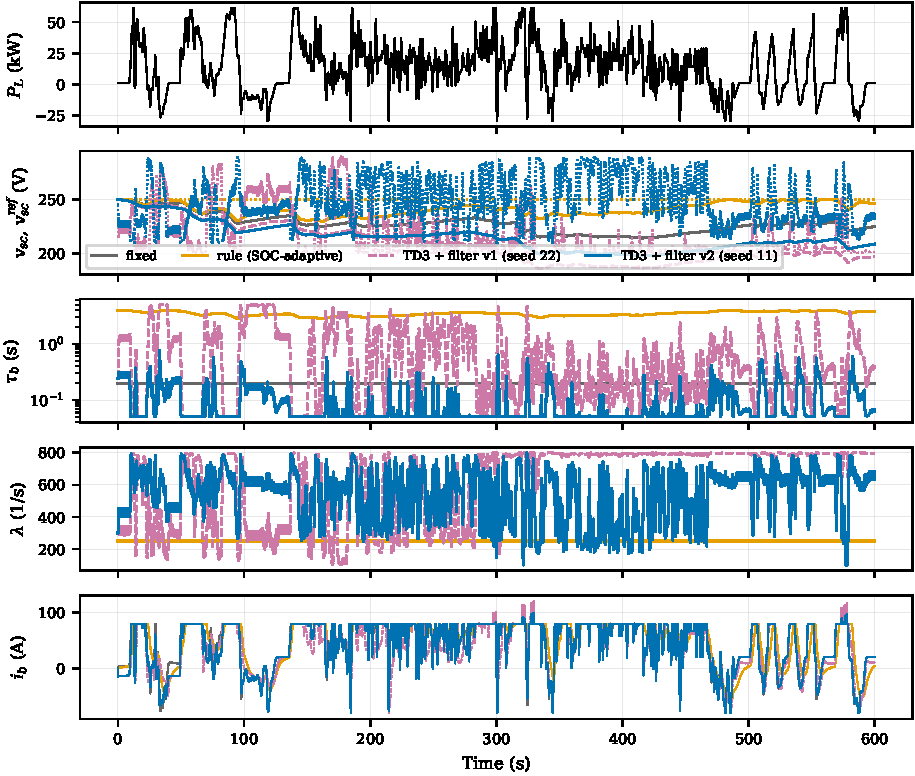
\includegraphics[width=\textwidth]{../results/figures/F4_us06_supervision.pdf}
\caption{US06 (held-out): load power, SC voltage (solid) with its reference (dotted), supervisory parameters $\tau_b$ and $\lambda$, and battery current for the fixed and SOC-rule supervisors and the median-validation agents of filter v1 and v2. The learned agents switch $v_{sc,ref}$ rapidly, so the recovery power is mostly at its $\pm\PrecMax$\,kW limit, and they keep $\tau_b$ near its lower bound. Filter v2 keeps $v_{sc,ref}\ge\VloVtwo$\,V, yet the net recharge is lower than with the fixed supervisor and the SC voltage falls below the level needed to supply the demand.}
\label{fig:us06}
\end{figure*}

\subsection{Effect of the safety filter}\label{sec:res_filter}
The filter changes the failure behavior more than the average performance.
\begin{itemize}
\item \emph{No filter.} One of the three seeds drove the bus out of its admissible range (simulation terminated) on US06, US06$\times1.1$, and WLTC extra-high$\times1.2$. This gives \R{us06a:nof:fails}/9, \R{us06b:nof:fails}/9 and \R{wxb:nof:fails}/9 failed runs. The mean saturation on US06 was \R{us06a:nof:sat:mean}\,\%.
\item \emph{Filter v1.} No run failed; saturation on US06 was \R{us06a:v1:sat:mean}\,\%.
\item \emph{Filter v2.} No agent run failed; saturation on US06 was \R{us06a:v2:sat:mean}\,\%. On WLTC extra-high$\times1.2$, saturation dropped from \R{wxb:v1:sat:mean}\,\% (v1) to \R{wxb:v2:sat:mean}\,\%.
\item \emph{Filter v2 with MPC-EMS.} The same filter did not prevent bus collapse for preview MPC-EMS on WLTC extra-high$\times1.2$ (\R{wxb:mpcv:fails}/\R{wxb:mpcv:runs} runs). The absence of failures in the agent runs is therefore an empirical result for these policies, not a guarantee provided by the filter.
\end{itemize}
The filter also narrows the spread between seeds (Table~\ref{tab:test}). On the main test cycles, the filter modified the $v_{sc,ref}$ component of the action in \FiltVscMin--\FiltVscMax\,\% of the decisions, through the rate limit or the bounds, which reflects the fast switching described above.

\subsection{Additional held-out cycles}\label{sec:res_extra}
\input{tab_extra.tex}

Table~\ref{tab:extra} reports three cycles that were introduced after filter v2 was fixed and influenced no design choice.
\begin{itemize}
\item \emph{WMTC.} v2 lowers the RMS battery current by \R{wmtc:v2vsafix:dibrmsabs}\,\% (fixed) and \R{wmtc:v2vsarule:dibrmsabs}\,\% (rule) without saturation, whereas v1 saturated \R{wmtc:v1:sat:mean}\,\% of the time.
\item \emph{FTP-MC1b} (mild). The reduction is \R{ftp:v2vsafix:dibrmsabs}\,\% (fixed) and \R{ftp:v2vsarule:dibrmsabs}\,\% (rule).
\item \emph{Long-haul segment} (mostly steady cruising). The agent \emph{increases} the RMS battery current from \R{lh:afix:ibrms}\,A to \R{lh:v2:ibrms:mean}\,A (+\R{lh:v2vsafix:dibrms}\,\%). The same switching of $P_{rec}$ between $\pm\PrecMax$\,kW now has no transient to cancel. It therefore adds a square-wave component of about $\PrecMax\,\mathrm{kW}/\SI{300}{V}\approx\SI{17}{A}$ to an otherwise nearly constant battery current; with the fixed supervisor, the mean $|P_{rec}|$ is \PrecLHfixedAbs\,kW.
\end{itemize}
This is a second, different failure mode outside the training distribution. MPC-EMS does not show it: on the long-haul segment its RMS battery current is \R{lh:mpcp:ibrms}\,A (persistence), below the \R{lh:afix:ibrms}\,A of the fixed supervisor, because switching $P_{rec}$ brings no predicted benefit when the load is nearly constant. Among the causal supervisors, persistence MPC-EMS also gives the lowest RMS battery current on FTP-MC1b (\R{ftp:mpcp:ibrms}\,A) and WMTC (\R{wmtc:mpcp:ibrms}\,A). On WMTC, however, it saturates \R{wmtc:mpcp:sat}\,\% of the time with a bus excursion of \R{wmtc:mpcp:maxdev}\,V, whereas the agent does not saturate.

\subsection{Computational cost}\label{sec:res_cost}
On the simulation host, one tier-1 update (compiled) costs \TimeADOSMC\,\si{\micro s}. One tier-2 decision (actor with \NActorParams\ parameters plus safety filter, interpreted Python) costs \TimeAgent\,\si{\micro s} every \SI{100}{ms}. One MPC-EMS decision (\NCandMPC\ candidates, \HorMPCP\,s horizon, vectorized NumPy) has a median cost of \TimeMPCEMS\,ms, more than an order of magnitude above the actor but still only about 1\,\% of the decision period. Both figures are relative indicators only; execution on an automotive microcontroller was not measured.


\subsection{Discussion}\label{sec:discussion}

\paragraph{What the evidence supports}
The tier-1 result is consistent across all test conditions.
\begin{itemize}
\item On both GTSD profiles and on every drive cycle, A-DO-SMC matches the observer-compensated robust MPC in bus-voltage regulation (Tables~\ref{tab:tier1}--\ref{tab:extra}). It has the update cost of the original fixed-gain DO-SMC and needs no online optimization.
\item The improvement over the fixed-gain DO-SMC comes from one mechanism: the reaching condition is enforced online using the observer's own error estimate. The sweep in Section~\ref{sec:repro} supports this: a large \emph{constant} gain gives comparable regulation. The adaptive law, however, applies a large gain only while the observer error is large, and the scaled boundary layer keeps the small-signal behaviour unchanged.
\end{itemize}
The supporting theory (Proposition~\ref{prop:uub}, Appendix~\ref{app:proof}) proves boundedness under input saturation and regional ultimate bounds in continuous time, under an estimator assumption that is checked numerically but not proved. For the sampled implementation it proves the observer bound and boundedness in unsaturated operation; sharp discrete-time bounds and saturated discrete-time operation remain open.

\paragraph{What the evidence does not support}
The learned supervisor is not uniformly beneficial.
\begin{itemize}
\item It lowered the RMS battery current on five of the six drive cycles evaluated at rated load (WLTC high and extra-high, US06, WMTC, FTP-MC1b), by up to \R{wh:v2vsafix:dibrmsabs}\,\% relative to the fixed supervisor.
\item On US06, the reduction came with power deficits that the fixed supervisor avoids.
\item On the long-haul segment, the RMS battery current tripled.
\item A non-learning MPC-EMS that optimizes the same objective over the same actions lowered the RMS battery current more than the agent on every test cycle, even with a causal persistence forecast, and without the long-haul failure.
\item Validation performance (Fig.~\ref{fig:val}) did not predict either failure. The validation cycles contain neither sustained high-power phases nor long steady cruising.
\end{itemize}
A claim that the agent reduces battery stress in general would therefore be wrong. The defensible claim is narrower: on cycles whose power and energy profile resembles the training cycles, the agent reduced RMS battery current more than a well-tuned SOC rule, at the cost of faster battery-current changes. It did not reach the battery-current reduction of a short-horizon model-based optimizer of the same objective. Its advantage over that optimizer is limited to fewer power deficits (US06, WMTC and WLTC extra-high$\times1.2$), which coincides with a higher average SC reference (\VtwoVrefMeanMin--\VtwoVrefMeanMax\,V against \MPCVrefMeanMin--\MPCVrefMeanMax\,V).

\paragraph{Why the agent fails: the action semantics were not enforced}
The supervisory variable $v_{sc,ref}$ was designed as a slow reserve setpoint. The reward, however, favors any use of it that lowers instantaneous battery stress. The agents found that rapid switching of the reference turns the bounded recovery term into a $\pm\PrecMax$\,kW battery-power actuator. Neither the rate limit of \SI{5}{V} per decision nor the reserve bound prevents this switching, because both constrain the \emph{value} of the reference rather than its \emph{effect}, i.e.\ the net SC energy balance. The MPC-EMS baseline fails differently but for a related reason. It parks $v_{sc,ref}$ at the filter's lower bound, because its \HorMPCP\,s prediction assigns no value to energy kept in the SC beyond the horizon. Two different optimizers of the same objective thus deplete the SC when sustained demand arrives. The root cause is the problem formulation (objective without a terminal value of stored energy, a short horizon, and a filter on a proxy variable), not the learning algorithm alone. This is a concrete instance of a general lesson for safe learning-based supervision: a safety filter must constrain the physical quantity that carries the risk (here, the SC energy and power capability over a horizon), not a proxy parameter.

\paragraph{The safety filter: necessary but not sufficient}
The filter did what it was designed to do.
\begin{itemize}
\item With the filter, no agent run left the admissible bus-voltage range. Without it, one training seed did so on three of the five test items. The filter alone did not guarantee this: preview MPC-EMS behind the same filter collapsed the bus on WLTC extra-high$\times1.2$.
\item Filter v2 removed the deficits of v1 on WLTC extra-high$\times1.2$ and WMTC, and reduced them on US06.
\end{itemize}
It did not make the agent safe in the operational sense, because its reserve bound is derived from the training distribution and acts on the reference only. Three remedies follow from the diagnosis; none of them is evaluated in this paper.
\begin{enumerate}
\item A runtime-assurance (simplex) switch that hands control to the fixed supervisor when the SC voltage approaches $v_{pow}$ in \eqref{eq:vpow}.
\item A filter on the \emph{net} recovery power over a moving window rather than on $v_{sc,ref}$.
\item Training on cycles that include sustained high-power and steady-cruise phases, and an objective with a terminal value of the SC energy, which would benefit learned and model-based supervisors alike.
\end{enumerate}
Because the v2 filter was itself designed after seeing test failures of v1, any further iteration should be evaluated on new held-out data.

\paragraph{Comparison with related work}
Safe-RL allocation with a predictive filter~\cite{xu2025safe} enforces operating constraints through model-based look-ahead. The simpler projection filter used here shows why such look-ahead matters: constraints on the next action alone did not anticipate SC depletion. Conversely, that work does not report a stability certificate for the voltage loop, whereas tier 1 provides one independently of the agent. The hierarchical controller of~\cite{jouili2026cbf} does give a Lyapunov--barrier certificate, but its agent outputs current references and its sliding-mode gains are scheduled from an estimator covariance; the certificate therefore does not have to accommodate agent-chosen observer gains. Combining a certificate-enforcing inner loop with a predictive or runtime-assured supervisor is therefore a natural next step. The RL-tuned observer gains of~\cite{choi2024dob,luna2026} adapt the observer for performance. Here, the agent's choice of $\lambda$ is made harmless to stability by the adaptive switching gain, and in the runs reported here the agents used $\lambda$ well above the nominal value (Fig.~\ref{fig:us06}).

\paragraph{Limits of the evidence}
\begin{itemize}
\item All results are offline simulations with an averaged converter model, an equivalent-circuit battery with constant parameters, and a road-load vehicle model whose parameters are assumed.
\item No hardware-in-the-loop or experimental validation was performed. Timing figures refer to a server CPU.
\item Agents were trained with a small budget (72\,000 transitions per seed, three seeds); larger budgets may change the learned behavior.
\item The GTSD load profiles were reconstructed from published figures.
\item Battery aging is represented only through current-based proxies (RMS, rate of change, charge throughput), not through an aging model.
\end{itemize}


\section{Conclusion}\label{sec:conclusion}
This paper combined a certificate-enforcing adaptive DO-SMC with a safety-filtered TD3 supervisor for a battery--supercapacitor EV storage system, and evaluated both tiers on held-out standard drive cycles.

\paragraph{Tier 1}
The adaptive DO-SMC estimates the observer error from $\dot{\hat D}=\lambda\tilde D$ and schedules the switching gain on it, which enforces the reaching condition online. On the transient profile of the reproduced design, the bus-voltage deviation fell from \R{pt:dosmc:maxdev}\,V to \R{pt:afix:maxdev}\,V. This matches an observer-compensated robust MPC, at the computational cost of the original fixed-gain controller.

\paragraph{Tier 2}
The TD3 supervisor with the safety filter reduced the RMS battery current on cycles resembling the training data, by \R{wh:v2vsafix:dibrmsabs}\,\% (WLTC high) and \R{ftp:v2vsafix:dibrmsabs}\,\% (FTP-MC1b) relative to fixed parameters. It never drove the bus out of range, whereas an unfiltered agent did. It also exhibited two failure modes on unseen cycles: power deficits on US06 (\R{us06a:v2:sat:mean}\,\% saturated time, against none for fixed parameters) and a tripled RMS battery current on steady cruising. Both trace back to the agent using the SC reference as a fast power actuator, which a filter acting on the reference value cannot prevent.

\paragraph{Practical recommendation}
The certificate-enforcing inner loop can be used on its own. A learned supervisor should not be deployed without a runtime-assurance fallback and a filter that constrains the net SC energy balance. Future work will add these elements, evaluate them on new held-out data, and validate both tiers in controller-hardware-in-the-loop.


\section*{Code and Data Availability}
The simulation code, the NumPy implementation of TD3, the trained supervisory agents (three variants, three training seeds each), the processed result files, and the scripts that regenerate every table and figure of this paper will be made publicly available at \url{https://github.com/VothanhHa-lab/hess-adosmc-td3} under the MIT licence (code) and CC~BY~4.0 (trained agents, processed results, tables and figures). The release will be archived on Zenodo with the persistent identifier DOI \textcolor{red}{[DOI to be inserted after Zenodo archiving]}.

The repository does not include the raw per-run simulation logs (about \SI{0.4}{GB}); these are regenerated by \texttt{scripts/evaluate.py} and are available from the authors on request. The one-hertz drive-cycle speed profiles are third-party data from the NREL FASTSim repository~\cite{fastsimrepo}; the repository ships only the files that the code reads, at the pinned commit recorded in \texttt{data/cycles/SOURCE\_COMMIT.txt}, and they remain subject to their original terms rather than to our licences. Vehicle, battery and resistance parameters are assumptions documented in \texttt{configs/nominal.yaml}; no experimental or hardware-in-the-loop data were used.


\section*{Declaration of competing interest}
The authors declare no competing interests.

\appendix
\section{Proof of Proposition 1}\label{app:proof}





This appendix proves Proposition~\ref{prop:uub} in continuous time with input saturation (Sections~\ref{ap:setting}--\ref{ap:proof}), states what the proof does not cover (Section~\ref{ap:limits}), and treats the sampled-data implementation (Section~\ref{ap:disc}). Every step that is proven is labeled as such. Everything that is only assumed or only checked numerically is labeled as such.

\subsection{Setting and Constants}\label{ap:setting}
Throughout, $g=1/C_{dc,n}$ and the design model is \eqref{eq:edyn} with $u$ the \emph{applied} (saturated) command of \eqref{eq:law}. The lumped disturbance $D$ is \emph{defined} by $D:=\dot e-gu$, so that $D$ contains the inner-loop error, the parameter mismatch and the allocation residual. We use the following standing hypotheses.
\begin{itemize}
\item[(H1)] $D$ is Lipschitz with $|\dot D|\le\rho_D$ along the closed-loop trajectory. This is the standard assumption on $D$ in DOBC analysis~\cite{chen2016dobc}. It is \emph{assumed}: because $D$ contains the inner-loop error, it is not exogenous, and a small-gain argument closing this loop is not given here.
\item[(H2)] $\lambda(t)\in[\lambda_{\min},\lambda_{\max}]$ is piecewise constant, with bumpless switching $z^+=\Dh^--\lambda^+e$. The filter state and the envelope start at zero, $\eta(t_0)=0$, $\varepsilon(t_0)=0$. Measurement noise is not modeled.
\item[(H3)] \emph{Capability margin.} There is $m>0$ with
\begin{equation}
g\,u_{\min}(t)+m\ \le\ -D(t)\ \le\ g\,u_{\max}(t)-m\quad\forall t.\label{ap:cap}
\end{equation}
This says that the load that must be compensated lies inside the source capability with margin $m$ (in V/s; $mC_{dc,n}$ in amperes).
\end{itemize}
Define $\Lambda=\lambda_{\max}/\lambda_{\min}$, $D_\infty=\rho_D/\lambda_{\min}$, $\bar D=\max(|\Dt(t_0)|,D_\infty)$, $\bar k_s=k_{\min}+\beta\Lambda\bar D$, $\bar\phi=\bar k_s/k'$, $W=\bar D+\bar k_s$, $E=\max(|e(t_0)|,W/c_v)$, and $\phi_{\min}=k_{\min}/k'$. We write $\mathrm{sat}$ for the unit saturation and $\mathrm{clip}(x;a,b)=\min(\max(x,a),b)$.

\subsection{Auxiliary Lemmas}\label{ap:lemmas}

\begin{lemma}[Observer error, envelope and gain]\label{lem:ndo}
Under (H1)--(H2), irrespective of saturation: (a) $\dot\Dh=\lambda\Dt$ and $\Dt$ is continuous; (b) $|\Dt(t)|\le|\Dt(t_0)|e^{-\lambda_{\min}(t-t_0)}+D_\infty$ and $|\Dt(t)|\le\bar D$; (c) $\varepsilon(t)\le\Lambda\bar D$, hence $k_{\min}\le k_s(t)\le\bar k_s$, and $\limsup\varepsilon\le\Lambda D_\infty$; (d) $\varepsilon$ is continuous except for upward jumps at switching instants of $\lambda$, and $\varepsilon(t')\ge\varepsilon(t)e^{-(t'-t)/\tau_{env}}$ for $t'>t$. Consequently $\dot k_s\ge-(k_s-k_{\min})/\tau_{env}$ almost everywhere.
\end{lemma}
\begin{proof}
(a) From \eqref{eq:ndo}, $\dot\Dh=\dot z+\lambda\dot e=-\lambda z-\lambda gu-\lambda^2e+\lambda(gu+D)=\lambda(D-\Dh)$. The command $u$ enters $\dot z$ and $\dot e$ identically. This holds for the applied $u$ also when it is saturated (the code feeds the clipped command $u$ to the observer update in \texttt{kernel\_sup.py}), so saturation does not enter $\dot\Dt$. At a switch, $z^+=\Dh^--\lambda^+e$ gives $\Dh^+=\Dh^-$ with $e$ continuous, so $\Dh$ and $\Dt=D-\Dh$ are continuous.

(b) Almost everywhere $\dot\Dt=\dot D-\lambda(t)\Dt$, so $\tfrac{d}{dt}\tfrac12\Dt^2\le|\Dt|(\rho_D-\lambda_{\min}|\Dt|)$. The scalar comparison lemma gives the first bound, and the set $|\Dt|\le\max(|\Dt(t_0)|,D_\infty)$ is invariant.

(c) Let $\eta$ be the filter state, $\tau_f\dot\eta=\dot\Dh-\eta$, $\eta(t_0)=0$. Then $\eta(t)=\int_{t_0}^t\tau_f^{-1}e^{-(t-\tau)/\tau_f}\lambda(\tau)\Dt(\tau)\,d\tau$, so $|\eta|\le\lambda_{\max}\bar D$ and $\hat\varepsilon=|\eta|/\lambda(t)\le\Lambda\bar D$. The envelope is $\varepsilon(t)=\sup_{\tau\le t}\hat\varepsilon(\tau)e^{-(t-\tau)/\tau_{env}}\le\Lambda\bar D$. For the $\limsup$, insert the bound (b) in the convolution. The transient part decays and the rest is at most $\lambda_{\max}D_\infty$.

(d) $\hat\varepsilon$ is continuous except at switches. There $\hat\varepsilon$ is multiplied by $\lambda^-/\lambda^+$, and the max in \eqref{eq:env} turns any downward jump into a continuous decay. The last statement follows from $k_s-k_{\min}=\beta\varepsilon$.
\end{proof}

\begin{lemma}[Saturation acts as a sector {$[0,1]$}]\label{lem:sector}
Under (H3), let $q:=\Dt-c_ve-k_s\,\mathrm{sat}(s/\phi_s)$ be the unsaturated error rate. Then $\dot e=\mathrm{clip}(q;\,gu_{\min}+D,\,gu_{\max}+D)$ with $gu_{\min}+D\le-m<0<m\le gu_{\max}+D$. Hence $\operatorname{sgn}\dot e=\operatorname{sgn}q$ and $\min(|q|,m)\le|\dot e|\le|q|$. The command is unsaturated whenever $|q|<m$.
\end{lemma}
\begin{proof}
With $v_c:=-\Dh-c_ve-k_s\,\mathrm{sat}(s/\phi_s)$ we have $gu=\mathrm{clip}(v_c;gu_{\min},gu_{\max})$ and $q=v_c+D$ (because $\Dt=D-\Dh$). Adding $D$ to a clip shifts both its argument and its limits, and \eqref{ap:cap} gives the sign of the shifted limits. The rest is elementary.
\end{proof}

\begin{lemma}[Boundary-layer geometry]\label{lem:layer}
Let Assumption~\ref{as:est} hold with $\gamma:=k_{\min}-\delta>0$ and $\tilde\beta=\beta(1-1/(k'\tau_{env}))$. Then, almost everywhere,
\begin{equation}
|\Dt|-k_s+\frac{k_s-k_{\min}}{k'\tau_{env}}\ \le\ -\gamma.\label{ap:R}
\end{equation}
\end{lemma}
\begin{proof}
$k_s-|\Dt|-(k_s-k_{\min})/(k'\tau_{env})=k_{\min}+\tilde\beta\varepsilon-|\Dt|\ge k_{\min}-\delta=\gamma$.
\end{proof}
Inequality \eqref{ap:R} is the precise reason for $\tilde\beta<\beta$ in Assumption~\ref{as:est}: the layer half-width $\phi_s=k_s/k'$ can shrink at the rate $(k_s-k_{\min})/(k'\tau_{env})$ (Lemma~\ref{lem:ndo}(d)), and the reaching margin $k_s-|\Dt|$ must beat that rate.

\subsection{Proof of the Proposition}\label{ap:proof}

\paragraph{Part (i): observer.} This is Lemma~\ref{lem:ndo}(a)--(b), which also proves \eqref{eq:ndobound} for piecewise constant, bumpless $\lambda(t)$.

\paragraph{Part (ii): boundedness under input saturation [(H1)--(H3) only].}
Let $w:=\Dt-k_s\,\mathrm{sat}(s/\phi_s)$, so $q=w-c_ve$ and $|w|\le|\Dt|+k_s\le W$ by Lemma~\ref{lem:ndo}.

\emph{Bound on $e$.} Suppose $|e(t_1)|>E$ for some $t_1$, say $e(t_1)>E$, and let $t_2<t_1$ be the last time with $e(t_2)=E$ (it exists because $|e(t_0)|\le E$). On $(t_2,t_1]$, $q\le W-c_ve<W-c_vE\le0$, so $\dot e<0$ by Lemma~\ref{lem:sector}. Then $e(t_1)<e(t_2)=E$, which is a contradiction. Hence $|e(t)|\le E$ for all $t$, with or without saturation. For the ultimate bound, let $W_\infty:=D_\infty+k_{\min}+\beta\Lambda D_\infty\ge\limsup(|\Dt|+k_s)$. For any $\theta>0$, after a finite time $|w|\le W_\infty+\theta$. For $|e|\ge(W_\infty+2\theta)/c_v$ we get $|q|\ge c_v|e|-|w|\ge\theta$, so $|\dot e|\ge\min(\theta,m)>0$ by Lemma~\ref{lem:sector}. Thus $e$ enters $|e|<(W_\infty+2\theta)/c_v$ in finite time and, by the invariance argument above, stays. Since $\theta$ is arbitrary,
\[
\limsup|e|\ \le\ \frac{D_\infty+k_{\min}+\beta\Lambda D_\infty}{c_v}.
\]
The time needed depends only on $|e(t_0)|$, $\bar D$, $\theta$, $m$. So $e$ is uniformly ultimately bounded.

\emph{Bound on $\xi$ (anti-windup).} $\xi$ is integrated only if $|s|\le\phi_s\le\bar\phi$ (this is true for both the rule \eqref{eq:condint} and the implemented rule with the additional sign condition). At such an instant $c_v\xi=s-e$, so $c_v|\xi|\le\bar\phi+E$. When the integrator is frozen, $\xi$ is constant. Hence $|\xi(t)|\le\max\big(|\xi(t_0)|,(\bar\phi+E)/c_v\big)$ for all $t$, and $|s|\le E+c_v|\xi|$ is bounded. This proves boundedness of $\xi$ and $s$ under saturation. It does \emph{not} prove that $\xi$ is ultimately bounded independently of $\xi(t_0)$: a frozen integrator can stay frozen (Remark~\ref{rem:deadlock}).

\paragraph{Part (iii): sharp bounds (regional).} Assume in addition Assumption~\ref{as:est}, the margin $m>\bar D+c_vE+\bar k_s$ and $|s(t_0)|<\phi_s(t_0)$.

\emph{Step 1: no saturation.} $|q|\le|\Dt|+c_v|e|+k_s\le\bar D+c_vE+\bar k_s<m$, so by Lemma~\ref{lem:sector} the command is never saturated and the integrator rule reduces to ``integrate iff $|s|\le\phi_s$''. For $E=W/c_v$ the condition reads $m>2W$.

\emph{Step 2: dynamics.} In both modes $\dot e=q=\Dt-c_ve-k_s\,\mathrm{sat}(s/\phi_s)$. If $|s|\le\phi_s$ the integrator runs ($\dot\xi=e$) and $\dot s=\dot e+c_ve=\Dt-k's$ (mode I). If $|s|>\phi_s$, then $\dot\xi=0$ and $\dot s=\dot e=\Dt-c_ve-k_s\operatorname{sgn}s$ (mode F). The two vector fields differ by $c_ve$ across $|s|=\phi_s$, so the right-hand side is discontinuous; solutions are understood in the Carath\'eodory sense and all statements are about any such solution. In mode I the right-hand side is continuous and Lipschitz.

\emph{Step 3: a trajectory cannot reach the layer boundary from the inside.} Let $v:=|s|-\phi_s$. $v$ is absolutely continuous between switches of $\lambda$, and $\phi_s$ jumps only upward (Lemma~\ref{lem:ndo}(d)), so jumps only decrease $v$. Suppose $v<0$ on $[t_0,t_1)$ and $v(t_1)=0$; say $s(t_1)=\phi_s(t_1)>0$. On $[t_0,t_1]$ mode I holds. By Lemma~\ref{lem:ndo}(d), almost everywhere on a left neighborhood of $t_1$,
\[
\dot v=\Dt-k's-\dot\phi_s\le\Dt-k_s-k'v+\frac{k_s-k_{\min}}{k'\tau_{env}}\le-\gamma+k'|v|,
\]
where we used $k's=k_s+k'v$ and \eqref{ap:R}. For $|v|<\gamma/(2k')$ this gives $\dot v\le-\gamma/2<0$, so $v$ cannot increase to $0$. The case $s(t_1)=-\phi_s(t_1)$ is symmetric. Hence $|s(t)|<\phi_s(t)$ for all $t\ge t_0$, mode I holds for all $t$, and the layer is positively invariant.

\emph{Step 4: sharp ultimate bounds.} By Step 3 the loop is linear and independent of $k_s$ for all $t$:
\begin{equation}
\dot s=\Dt-k's,\qquad \dot e=-c_ve+\Dt-k's.\label{ap:lin}
\end{equation}
Hence $s(t)=s(t_0)e^{-k'(t-t_0)}+\int e^{-k'(t-\tau)}\Dt\,d\tau$, which gives $\limsup|s|\le D_\infty/k'$. The map $\Dt\mapsto e$ has transfer function $p/((p+c_v)(p+k'))$ plus decaying free responses, with impulse response $h(t)=(c_ve^{-c_vt}-k'e^{-k't})/(c_v-k')$. Its $L^1$ norm is
\[
\kappa:=\|h\|_1=\frac{2}{k'}\Big(\frac{c_v}{k'}\Big)^{\frac{c_v}{k'-c_v}}\ \le\ \frac{2}{k'}\qquad(k'>c_v),
\]
(the closed form follows because $h$ changes sign once, at $t^\ast=\ln(k'/c_v)/(k'-c_v)$ and $\int_0^\infty h=0$). Since $|\Dt|\le|\Dt(t_0)|e^{-\lambda_{\min}(t-t_0)}+D_\infty$, we get $\limsup|e|\le\kappa D_\infty$. From $c_v\xi=s-e$, $\limsup|\xi|\le(1/k'+\kappa)D_\infty/c_v$. These bounds are uniform in the initial conditions, because the transients are exponentially decaying with rates $\min(c_v,k',\lambda_{\min})$ or faster, and are multiplied by $|s(t_0)|$, $|e(t_0)|$, $|\Dt(t_0)|$ only. Since $\beta\Lambda>1$ gives $D_\infty<\bar k_s$ and hence $D_\infty/k'<\bar\phi$, the set $|s|\le\bar\phi$ of the original statement is contained in the proven layer $|s|<\phi_s(t)\le\bar\phi$.

\emph{Step 5: reaching from outside the layer (regional).} Suppose now $s(t_0)>\phi_s(t_0)$ (the case $s(t_0)<-\phi_s(t_0)$ is symmetric), with $a:=c_v\xi(t_0)$ and $a<\phi_{\min}+\gamma/c_v$, and the margin of Step~1. While $v>0$, $\xi\equiv\xi(t_0)$, $e=s-a$, and mode F with \eqref{ap:R} and $s>\phi_s\ge\phi_{\min}$ gives, almost everywhere,
\begin{align*}
\dot v=\dot s-\dot\phi_s&\le\Dt-k_s-c_v(s-a)+\tfrac{k_s-k_{\min}}{k'\tau_{env}}\le-g_0,\\
g_0&:=\gamma+c_v(\phi_{\min}-a)>0.
\end{align*}
So $v$ reaches $0$ at a time $t_r\le t_0+v(t_0)/g_0$. Immediately afterwards the trajectory enters the open layer: otherwise $v\ge0$ on some $[t_r,t_r+h]$. The set $\{v=0\}$ is then a null set (in mode I, $\dot v\le-\gamma$ at differentiability points by \eqref{ap:R}, while $\dot v=0$ almost everywhere on $\{v=0\}$). Hence $\xi$ stays within $E h$ of $\xi(t_0)$ and, for small $h$, $\dot v\le-g_0/2$ almost everywhere on $[t_r,t_r+h]$. Then $v(t_r+h)<0$, a contradiction. From then on Steps 3--4 apply. This proves finite-time reaching of $|s|<\phi_s$ in the stated region of $(s(t_0),\xi(t_0))$. For $e(t_0)=\xi(t_0)=0$ no reaching phase is needed.

\paragraph{Remark on reaching.} The identity $\dot s=\Dt-k_s\,\mathrm{sat}(s/\phi_s)$ holds only while $\xi$ integrates. Outside the layer $\xi$ is frozen and $\dot s$ contains the extra term $-c_ve$. A Lyapunov argument with $V=\tfrac12s^2$ outside the layer is therefore \emph{not} valid, and finite-time reaching cannot hold from arbitrary initial states; the correct statement is the regional one of Step~5.

\subsection{Scope and Limitations of the Proof}\label{ap:limits}
\begin{remark}[Frozen-integrator trap]\label{rem:deadlock}
If $s(t_0)>\phi_s$ and $a=c_v\xi(t_0)>\phi_s+(k_s-\Dt)/c_v$, then outside the layer $e\to-(k_s-\Dt)/c_v$ and $s\to a-(k_s-\Dt)/c_v>\phi_s$: the integrator stays frozen and $e$ keeps a constant offset of order $k_s/c_v$. In simulation of the design model with $D=0$, $k_s=k_{\min}$, $e(t_0)=0$ and $c_v\xi(t_0)=\SI{5}{V}$ the state ended at $s=\SI{3.8}{V}$, $\phi_s=\SI{0.5}{V}$, $e=\SI{-1.2}{V}$ after \SI{1.5}{s}, as predicted. With $c_v\xi(t_0)=\SI{0.4}{V}$ (inside the regional condition) $s\to0$. $e$ stays bounded in the trap (Part (ii)), but the sharp bounds do not hold.
\end{remark}
\begin{remark}[Power deficit]\label{rem:deficit}
If (H3) fails, no bound can be given for \emph{any} controller. If $-D(t)\ge gu_{\max}(t)+m'$ on an interval, then $\dot e=D+gu\le-m'$ there, so $e$ decreases at least linearly. In simulation of the design model with $D=\SI{-9e4}{V/s}$ and $gu_{\max}=\SI{7e4}{V/s}$, $e(\SI{0.2}{s})=\SI{-4078}{V}$ against the bound $-4000$\,V. This is the power-deficit case that occurs on the US06 cycle, where the proposition makes no claim.
\end{remark}
\begin{remark}[Not covered]
Measurement noise (it enters $\Dh=z+\lambda e$ with gain $\lambda$, so it acts as an extra disturbance and is not included in $D_\infty$); the closure of (H1) through the inner loop; the clipping of the inner loops (duty limits) beyond what is lumped in $D$; and the interaction of $\lambda$ with the SC reserve filter (the filter enters only through $\lambda\in[\lambda_{\min},\lambda_{\max}]$ and the bumpless re-initialization).
\end{remark}
\begin{remark}[Conservatism and values on US06]
The margin condition $m>2W$ is conservative. Substituting the supremum values measured in the noise-free US06 run on the Tesla Model 3 plant, $\sup|\Dt|=\DtildeMaxAdapt$\,V/s and $\sup k_s=\KsMaxAdapt$\,V/s (instead of $\bar D$ and $\bar k_s$) gives $W\approx\AppW\times10^{3}$\,V/s and $2W\approx\AppTwoW\times10^{3}$\,V/s, i.e. about \AppTwoWA\,A of bus current at $C_{dc,n}$. The capability from \eqref{eq:ulim} is about \AppCap\,A at $v_b\approx\AppVb$\,V, $v_{sc}=\AppVsc$\,V, $v_{dc}=\AppVdc$\,V. This is an illustration with measured suprema, not a certificate. The sharp bounds also need Assumption~\ref{as:est}. Writing the verified ratio as $k_s\ge r|\Dt|$, Assumption~\ref{as:est} follows with $\delta=k_{\min}/r$ whenever $r\ge\beta/\tilde\beta=12/11$. The reported minimum ratio is $r=\MinKsRatio$ (noise-free run, $t>0.2$\,s), which gives $\delta\approx\AppDelta\,V/s<k_{\min}$.
\end{remark}

\subsection{Discretization and One-Sample Delay}\label{ap:disc}
The implementation has $T_s=\SI{50}{\micro s}$, a one-sample computation delay, the forward-Euler observer \eqref{eq:zdisc} and the discrete envelope \eqref{eq:envdisc}. Here $k'T_s=0.012$, $c_vT_s=0.005$, $\lambda_{\max}T_s=0.04$, $T_s/\tau_f=0.025$.

\paragraph{Discrete plant model.} Let the plant over $[t_k,t_{k+1}]$ be $e_{k+1}=e_k+T_s(gu_{k-1}+\delta_k)$, where $u_{k-1}$ is the command computed one sample earlier, and $\delta_k$ is \emph{defined} by this equation (it contains the true disturbance, the inner-loop error and the sampling error). Define the effective disturbance seen by the observer, which is fed $u_k$, as $d_k:=(e_{k+1}-e_k)/T_s-gu_k=\delta_k+g(u_{k-1}-u_k)$.

\begin{lemma}[Discrete observer; proven]\label{prop:disc-ndo}
For the Euler observer with bumpless switching and $\lambda_{\max}T_s\le1$, $\Dh_{k+1}=(1-\lambda_kT_s)\Dh_k+\lambda_kT_sd_k$. With $\tilde D_k:=d_k-\Dh_k$ and $|d_{k+1}-d_k|\le T_s\rho_d$,
\begin{align*}
|\tilde D_k|&\le(1-\lambda_{\min}T_s)^{k}|\tilde D_0|+\rho_d/\lambda_{\min},\\
|\tilde D_k|&\le\max(|\tilde D_0|,\rho_d/\lambda_{\min}).
\end{align*}
Moreover $(\Dh_{k}-\Dh_{k-1})/T_s=\lambda_{k-1}\tilde D_{k-1}$, so $\varepsilon_k\le\Lambda\bar D_d$ with $\bar D_d=\max(|\tilde D_0|,\rho_d/\lambda_{\min})$.
\end{lemma}
\begin{proof}
$\Dh_{k+1}-\Dh_k=z_{k+1}-z_k+\lambda_k(e_{k+1}-e_k)=-\lambda_kT_s\Dh_k+\lambda_k[(e_{k+1}-e_k)-T_sgu_k]$, which is the first identity. Subtracting from $d_{k+1}$ gives $\tilde D_{k+1}=(1-\lambda_kT_s)\tilde D_k+(d_{k+1}-d_k)$ and hence the bounds because $0\le1-\lambda_kT_s\le1-\lambda_{\min}T_s$. The envelope claim follows as in Lemma~\ref{lem:ndo}(c), since the discrete filter is a convex average of the backward differences.
\end{proof}
The sufficient condition is $\lambda_{\max}T_s\le0.04<1$; the observer pole is $1-\lambda T_s\in[0.96,0.995]$. The assumption $|d_{k+1}-d_k|\le T_s\rho_d$ is \emph{assumed}: since $d_k=\delta_k+g(u_{k-1}-u_k)$, one has $\rho_d\le\rho_\delta+2R_u$ with $\rho_\delta=\sup|\delta_{k+1}-\delta_k|/T_s$ and $R_u=\sup g|u_k-u_{k-1}|/T_s$. $R_u$ is a closed-loop quantity that can be read from the logs. This is the price of the delay.

\begin{lemma}[Discrete boundedness; proven, unsaturated]\label{prop:disc-e}
Assume $c_vT_s<1$, $u_k=u^{un}_k$ for all $k$, and let $W_d:=\bar D_d+\bar k_s^d+T_s\rho_d$ with $\bar k_s^d=k_{\min}+\beta\Lambda\bar D_d$. If the initial values satisfy $|e_j|\le\hat E$ for all $j\le1$ and
\[
\hat E\ \ge\ \frac{W_d}{c_v}\,\frac{1+c_vT_s}{1-c_vT_s},
\]
then $|e_k|\le\hat E$ for all $k$, and $|\xi_k|\le\max\big(|\xi_0|,(\bar\phi_d+\hat E)/c_v\big)$ with $\bar\phi_d=\bar k_s^d/k'$.
\end{lemma}
\begin{proof}
With the delay, $e_{k+1}=e_k-T_sc_ve_{k-1}+T_sw_k$, $w_k:=\delta_k-\Dh_{k-1}-k_{s,k-1}\mathrm{sat}(\cdot)$. Using $\delta_k-\Dh_{k-1}=(\delta_k-d_{k-1})+\tilde D_{k-1}$ and $|\delta_k-d_{k-1}|\le T_s\rho_d$ gives $|w_k|\le W_d$. Write $e_{k+1}=(1-c_vT_s)e_k+c_vT_s(e_k-e_{k-1})+T_sw_k$ and $e_k-e_{k-1}=-T_sc_ve_{k-2}+T_sw_{k-1}$. If $|e_j|\le\hat E$ for $j\le k$, then $|e_{k+1}|\le(1-c_vT_s)\hat E+c_vT_s^2(c_v\hat E+W_d)+T_sW_d\le\hat E$ exactly when $\hat Ec_vT_s(1-c_vT_s)\ge T_sW_d(1+c_vT_s)$, which is the stated condition. Integration occurs only if $|s_k|\le\phi_{s,k}$; after such a step $c_v\xi_{k+1}=s_k-(1-c_vT_s)e_k$, so $c_v|\xi_{k+1}|\le\bar\phi_d+\hat E$. Frozen steps keep $\xi$.
\end{proof}
For the nominal $c_vT_s=0.005$ the inflation factor with respect to the continuous bound is $(1+c_vT_s)/(1-c_vT_s)=1.0101$. Saturation in discrete time and the discrete counterpart of Steps 3--5 (layer invariance and the sharp bounds) are \emph{not proven}.

\paragraph{Numerical verification of the sampled linearized loop (not a proof).} In the layer with the integrator active, the loop is linear. We built its exact sampled-data model with state $(e,\xi,z,a_{k-1})$ and $a_k=gu_k$: the plant is integrated exactly over each period with the command computed one sample before, the observer is the Euler observer of \eqref{eq:zdisc} fed with the current command, and $\xi_{k+1}=\xi_k+T_se_k$. We also added an inner-loop lag as a modeling assumption: a unity-gain first-order response with bandwidth $\omega_{ci}=\SI{5026.5}{rad/s}$ (Table~\ref{tab:ctrl}) between the applied command and the bus current. The script is \texttt{proof\_check.py}; the numbers below were computed with it. The continuous-time poles of the loop are $\{-c_v,-k',-\lambda\}$ (verified numerically for $\lambda=250$ and $800$\,s$^{-1}$).
\begin{center}\footnotesize
\begin{tabular}{@{}lcc@{}}
\toprule
 & delay only & delay + lag\\
\midrule
$\rho$ at $\lambda=100$ & 0.995040 & 0.995176\\
$\rho$ at $\lambda=800$ & 0.994997 & 0.994987\\
max $\rho$ on the grid & 0.995040 & 0.995176\\
delay margin, $\lambda=100$ / $800$ & 56 / 22 & 52 / 19\\
\bottomrule
\end{tabular}
\end{center}
(delay margin in samples; grid $\lambda=100,110,\dots,800$\,s$^{-1}$)
Here $\rho$ is the spectral radius of the closed-loop matrix. The slowest mode is the $c_v$ pole, $e^{-c_vT_s}=0.995012$, for every $\lambda$ on the grid. The delay margin is the largest number of whole computation-delay samples for which $\rho<1$ (the implementation uses one). At $\lambda=800$\,s$^{-1}$, $T_s$ could be scaled by a factor of 16.1 (14.6 with the inner-loop lag) before the one-sample-delay loop becomes unstable. This verifies stability of the linearized in-layer loop on a grid of 71 values of $\lambda$; it does not cover the nonlinear loop, saturation or the interpolation between grid points.

\paragraph{Simulation check of the continuous design model (not a proof).} The same script simulates $\dot e=gu+D$ with the full tier-1 law (NDO, envelope, time-varying layer, conditional integrator, clipping, bumpless rate-limited $\lambda$ switching in $[100,400]$\,s$^{-1}$, step $T_s/10$, 3\,s). For three random Lipschitz disturbances with $\rho_D=\SI{2e4}{V/s^2}$, and with a capability well above $|D|$, no violation of $|s|<\phi_s$ occurred ($\max|s|/\phi_s=0.44$) and $\sup|e|\le\SI{0.41}{V}$ against $W/c_v\approx\SI{5}{V}$. In a stress case with a trapezoidal $D$ ($\pm\SI{3e4}{V/s}$, ramps of about \SI{8}{ms}) and a capability limit only $\SI{500}{V/s}$ above $|D|$, the input was saturated in 50.5\,\% of the steps at $\lambda=100$\,s$^{-1}$ and 23.2\,\% at $\lambda=400$\,s$^{-1}$. There $\sup|e|=\SI{67.9}{V}$ and $\SI{31.1}{V}$ against the Part (ii) bound $W/c_v$ of \SI{726}{V} and \SI{432}{V}, evaluated with the measured $\sup|\Dt|$ and $\sup k_s$. The layer was left in these runs (peak $|s|/\phi_s=21.5$ and $1.09$), which is allowed because the sharp part needs Assumption~\ref{as:est} and the margin $m>2W$, neither of which held. $\xi$ stayed bounded ($\sup|\xi|\le$0.53$\,V\,s$).


\bibliographystyle{unsrtnat}
\bibliography{refs}
\end{document}
